% Versão 24/06/2020

% Este documento destina-se a servir como modelo para a produção de documentos
% de pesquisa do PPGINF/UFPR, como projetos, dissertações e teses. A classe de
% documento se chama "ppginf" (arquivo ppginf.cls) e define o formato básico do
% documento. O texto está organizado em capítulos que são colocados em
% subdiretórios separados. São definidos exemplos para a inclusão de figuras,
% códigos-fonte e a definição de tabelas.
%
% Produzido por Carlos Maziero (maziero@inf.ufpr.br).

%=====================================================

% Opções da classe ppginf:
%
% - defesa    : versão para entregar à banca; tem espaçamento 1,5
%               e omite algumas páginas iniciais (agradecimentos, etc)
% - final     : versão pós-defesa, para enviar à biblioteca;
%               tem espaçamento simples e todas as páginas iniciais.
% - oneside   : somente frente; use quando for gerar somente o PDF.
% - twoside   : frente/verso; use se precisar de uma versão impressa.
% - metadados : inclui metadados no PDF (por default não inclui)
% - ...       : demais opções aceitas pela classe "book"

% ATENÇÂO: este modelo tem suporte para português e inglês.
% As duas línguas devem ser informadas como opção da classe;
% a língua principal do documento deve vir POR ÚLTIMO.

% Versão de defesa
%\documentclass[defesa,oneside,english,brazilian]{ppginf}

% Versão de defesa em inglês
%\documentclass[defesa,oneside,brazilian,english]{ppginf}

% Versão final em PDF para a biblioteca da UFPR
\documentclass[final,oneside,english,brazilian]{ppginf}

% Versão final para impressão (frente/verso)
%\documentclass[final,twoside,english,brazilian]{ppginf}

% configurações de diversos pacotes, inclusive a fonte usada no texto
% Pacotes usados neste documento e suas respectivas configurações

% ------------------------------------------------------------------------------

% Definição de fontes

% formato dos arquivos-fonte (utf8 no Linux e latin1 no Windows)
\usepackage[utf8]{inputenc}	% arquivos LaTeX em Unicode (UTF8)

% usar codificação T1 para ter caracteres acentuados corretos no PDF
\usepackage[T1]{fontenc}

% fonte usada no corpo do texto (pode alterar, mas descomente apenas uma)
\usepackage{newtxtext,newtxmath}	% Times (se não tiver, use mathptmx)
%\usepackage{lmodern}			% Computer Modern (fonte clássico LaTeX)
%\usepackage{kpfonts}			% Kepler/Palatino (idem, use mathpazo)
%\renewcommand{\familydefault}{\sfdefault} % Arial/Helvética (leia abaixo)

% A biblioteca central da UFPR recomenda usar Arial, seguindo a recomendação da
% ABNT. Essa é uma escolha ruim, pois fontes sans-serif são geralmente inade-
% quados para textos longos e impressos, sendo melhores para páginas Web.
% http://www.webdesignerdepot.com/2013/03/serif-vs-sans-the-final-battle/.

% fontes usadas em ambientes específicos
\usepackage[scaled=0.9]{helvet}		% Sans Serif
\usepackage{courier}			% Verbatim, Listings, etc

% ------------------------------------------------------------------------------

% inclusão de figuras em PDF, PNG, PS, EPS
\usepackage{graphicx}

% subfiguras (subfigure is deprecated, don't use it)
\usepackage[labelformat=simple]{subcaption}
\renewcommand\thesubfigure{(\alph{subfigure})}

% ------------------------------------------------------------------------------

% inclusão/formatação de código-fonte (programas)
\usepackage{listings}
\lstset{language=c}
\lstset{basicstyle=\ttfamily\footnotesize,commentstyle=\textit,stringstyle=\ttfamily}
\lstset{showspaces=false,showtabs=false,showstringspaces=false}
\lstset{numbers=left,stepnumber=1,numberstyle=\tiny}
\lstset{columns=flexible,mathescape=true}
\lstset{frame=single}
\lstset{inputencoding=utf8,extendedchars=true}
\lstset{literate={á}{{\'a}}1  {ã}{{\~a}}1 {à}{{\`a}}1 {â}{{\^a}}1
                 {Á}{{\'A}}1  {Ã}{{\~A}}1 {À}{{\`A}}1 {Â}{{\^A}}1
                 {é}{{\'e}}1  {ê}{{\^e}}1 {É}{{\'E}}1  {Ê}{{\^E}}1
                 {í}{{\'\i}}1 {Í}{{\'I}}1
                 {ó}{{\'o}}1  {õ}{{\~o}}1 {ô}{{\^o}}1
                 {Ó}{{\'O}}1  {Õ}{{\~O}}1 {Ô}{{\^O}}1
                 {ú}{{\'u}}1  {Ú}{{\'U}}1
                 {ç}{{\c{c}}}1 {Ç}{{\c{C}}}1 }

% ------------------------------------------------------------------------------

% formatação de algoritmos
\usepackage{algorithm,algorithmic}
\IfLanguageName{brazilian} {\floatname{algorithm}{Algoritmo}}{}
\renewcommand{\algorithmiccomment}[1]{~~~// #1}
%\algsetup{linenosize=\footnotesize,linenodelimiter=.}

% ------------------------------------------------------------------------------

% formatação de bibliografia
\usepackage{natbib}		% bibliografia no estilo NatBib
\renewcommand{\cite}{\citep}	% \cite deve funcionar como \citep
%\bibpunct{[}{]}{;}{a}{}{,}	% caracteres usados nas referências

% ------------------------------------------------------------------------------

% fontes adicionais
\usepackage{amsmath}		% pacotes matemáticos
\usepackage{amsfonts}		% fontes matemáticas 
\usepackage{amssymb}		% símbolos 

% ------------------------------------------------------------------------------

% pacotes diversos
\usepackage{alltt,moreverb}	% mais comandos no modo verbatim
\usepackage{lipsum}		% gera texto aleatório (para os exemplos)
\usepackage{currfile}		% infos sobre o arquivo/diretório atual
\usepackage[final]{pdfpages}	% inclusão de páginas em PDF
\usepackage{longtable}		% tabelas multi-páginas (tab símbolos/acrônimos)

% ------------------------------------------------------------------------------



%=====================================================

\begin {document}

% Principais dados, usados para gerar as páginas iniciais.
% Campos não utilizados podem ser removidos ou comentados.

% título
\title{Reduzindo o consumo de energia do Hadoop 3.x MapReduce através do Energy Efficient Ethernet}

% palavras-chave e keywords (p/ resumo, abstract e metadados do PDF)
\pchave{Green Networking, Big Data, Energy Efficient Ethernet, MapReduce, Hadoop.}
\keyword{Green Networking, Big Data, Energy Efficient Ethernet, MapReduce, Hadoop.}

% autoria
\author{Jorgi Luiz Bolonhezi Dias}
\advisor{Luiz Carlos Pessoa Albini}
\coadvisor{Leandro Batista De Almeida}

% instituição
\IfLanguageName{brazilian}
  { \instit{UFPR}{Universidade Federal do Paraná} }
% a Bib/UFPR exige que tudo seja em português, exceto o título :-(
%  { \instit{UFPR}{Federal University of Paraná} }
  { \instit{UFPR}{Universidade Federal do Paraná} }

% área de concentração (default do PPGInf, não mudar)
\IfLanguageName{brazilian}
  { \field{Ciência da Computação} }
% a Bib/UFPR exige que tudo seja em português, exceto o título :-(
%  { \field{Computer Science} }
  { \field{Ciência da Computação} }

% data (só o ano)
\date{2022}

% local
\IfLanguageName{brazilian}
  { \local{Curitiba - PR} }
% a Bib/UFPR exige que tudo seja em português, exceto o título :-(
%  { \local{Curitiba PR - Brazil} }
  { \local{Curitiba - PR} }

% imagem de fundo da capa (se não desejar, basta comentar)
\coverimage{0-iniciais/fundo-capa.jpg}

%=====================================================

%% Descrição do documento (obviamente, descomentar somente UMA!)

% Por exigência da biblioteca da UFPR, a descrição do documento deve ser
% em português, mesmo em documentos em outras línguas. Vá entender...

% tese de doutorado
%\descr{Qualificação apresentada como requisito parcial à obtenção do grau de Mestre em Ciência da Computação no Programa de Pós-Graduação em Informática, Setor de Ciências Exatas, da Universidade Federal do Paraná}

% exame de qualificação de doutorado
%\descr{Documento apresentado como requisito parcial ao exame de qualificação de Doutorado no Programa de Pós-Graduação em Informática, Setor de Ciências Exatas, da Universidade Federal do Paraná}

% dissertação de mestrado
\descr{Dissertação apresentada como requisito parcial à obtenção do grau de Mestre em Informática no Programa de Pós-Graduação em Informática, Setor de Ciências Exatas, da Universidade Federal do Paraná}

% exame de qualificação de mestrado
%\descr{Documento apresentado como requisito parcial ao exame de qualificação de Mestrado no Programa de Pós-Graduação em Informática, Setor de Ciências Exatas, da Universidade Federal do Paraná}

% trabalho de conclusão de curso
%\descr{Trabalho apresentado como requisito parcial à conclusão do Curso de Bacharelado em XYZ, Setor de Ciências Exatas, da Universidade Federal do Paraná}

% trabalho de disciplina
%\descr{Trabalho apresentado como requisito parcial à conclusão da disciplina XYZ no Curso de Bacharelado em XYZ, Setor de Ciências Exatas, da Universidade Federal do Paraná}

% doctorate thesis
%\descr{Thesis presented as a partial requirement for the degree of Doctor in Computer Science in the Graduate Program in Informatics, Exact Sciences Sector, of the Federal University of Paraná, Brazil}

% doctorate qualification
%\descr{Document presented as a partial requirement for the doctoral qualification exam in the Graduate Program in Informatics, Exact Sciences Sector, of the Federal University of Paraná, Brazil}

% MSc dissertation
%\descr{Dissertation presented as a partial requirement for the degree of Master of Sciences in Informatics in the Graduate Program in Informatics, Exact Sciences Sector, of the Federal University of Paraná, Brazil.}

% MSc qualification
%\descr{Document presented as a partial requirement for the Master of Sciences qualification exam in the Graduate Program in Informatics, Exact Sciences Sector, of the Federal University of Paraná, Brazil}

%=====================================================

% define estilo das páginas iniciais (capas, resumo, sumário, etc)
\frontmatter
\pagestyle{frontmatter}

% produz capa e folha de rosto
\titlepage

% páginas que só aparecem na versão final (a inclusão é automática)
% IMPORTANTE: o conteúdo exato da ficha catalográfica é preparada pela
% Biblioteca da UFPR. Não "invente" um conteúdo para ela!

\begin{ficha}	% só gera conteúdo se for na versão final

% inclusão da ficha catalográfica final (arquivo PDF)
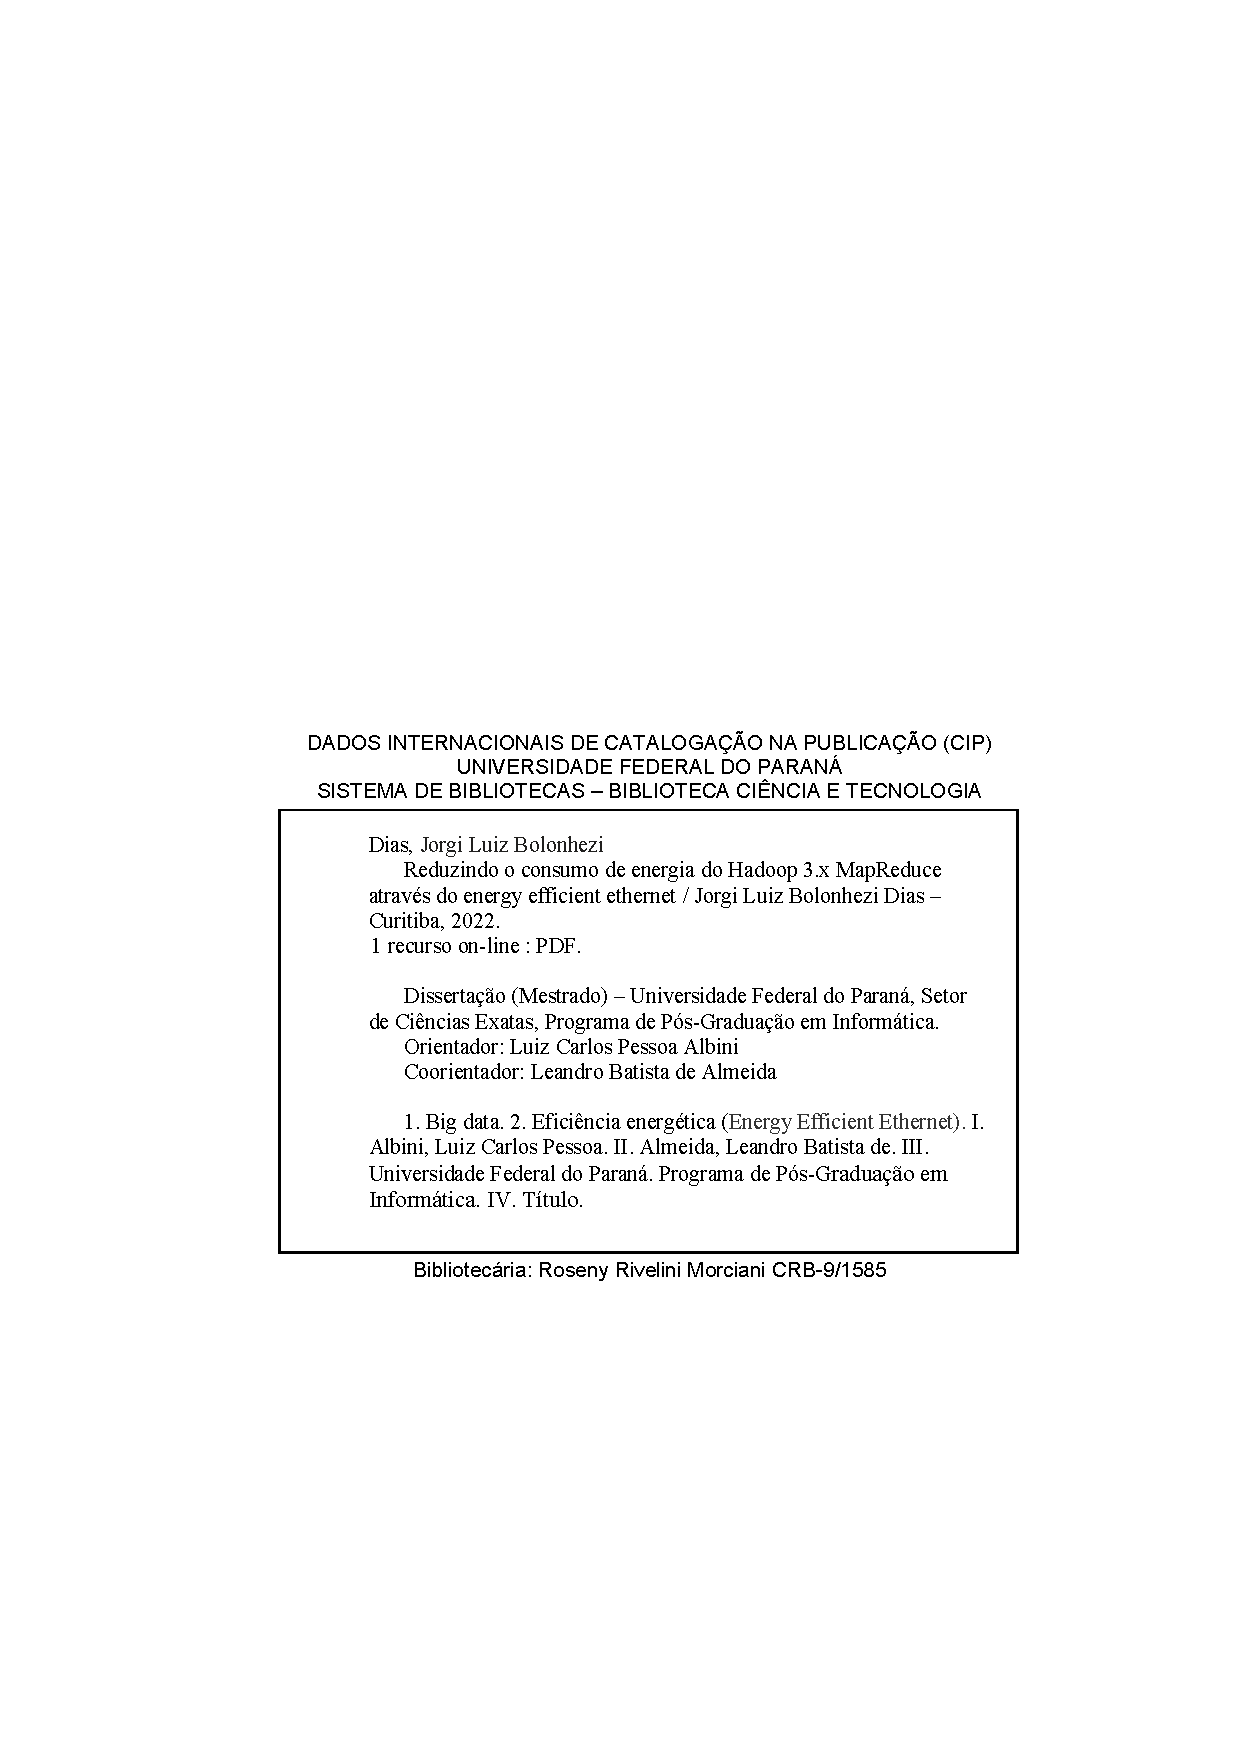
\includepdf[noautoscale]{0-iniciais/Ficha_Catalografica.pdf}

\end{ficha}

%=====================================================
	% ficha catalográfica
% A ficha de aprovação será fornecida pela secretaria do programa,
% após a defesa e cumprimento dos demais trâmites legais.

\begin{aprovacao}	% só gera conteúdo se for na versão final

% inclusão do termo de aprovação final (arquivo PDF)
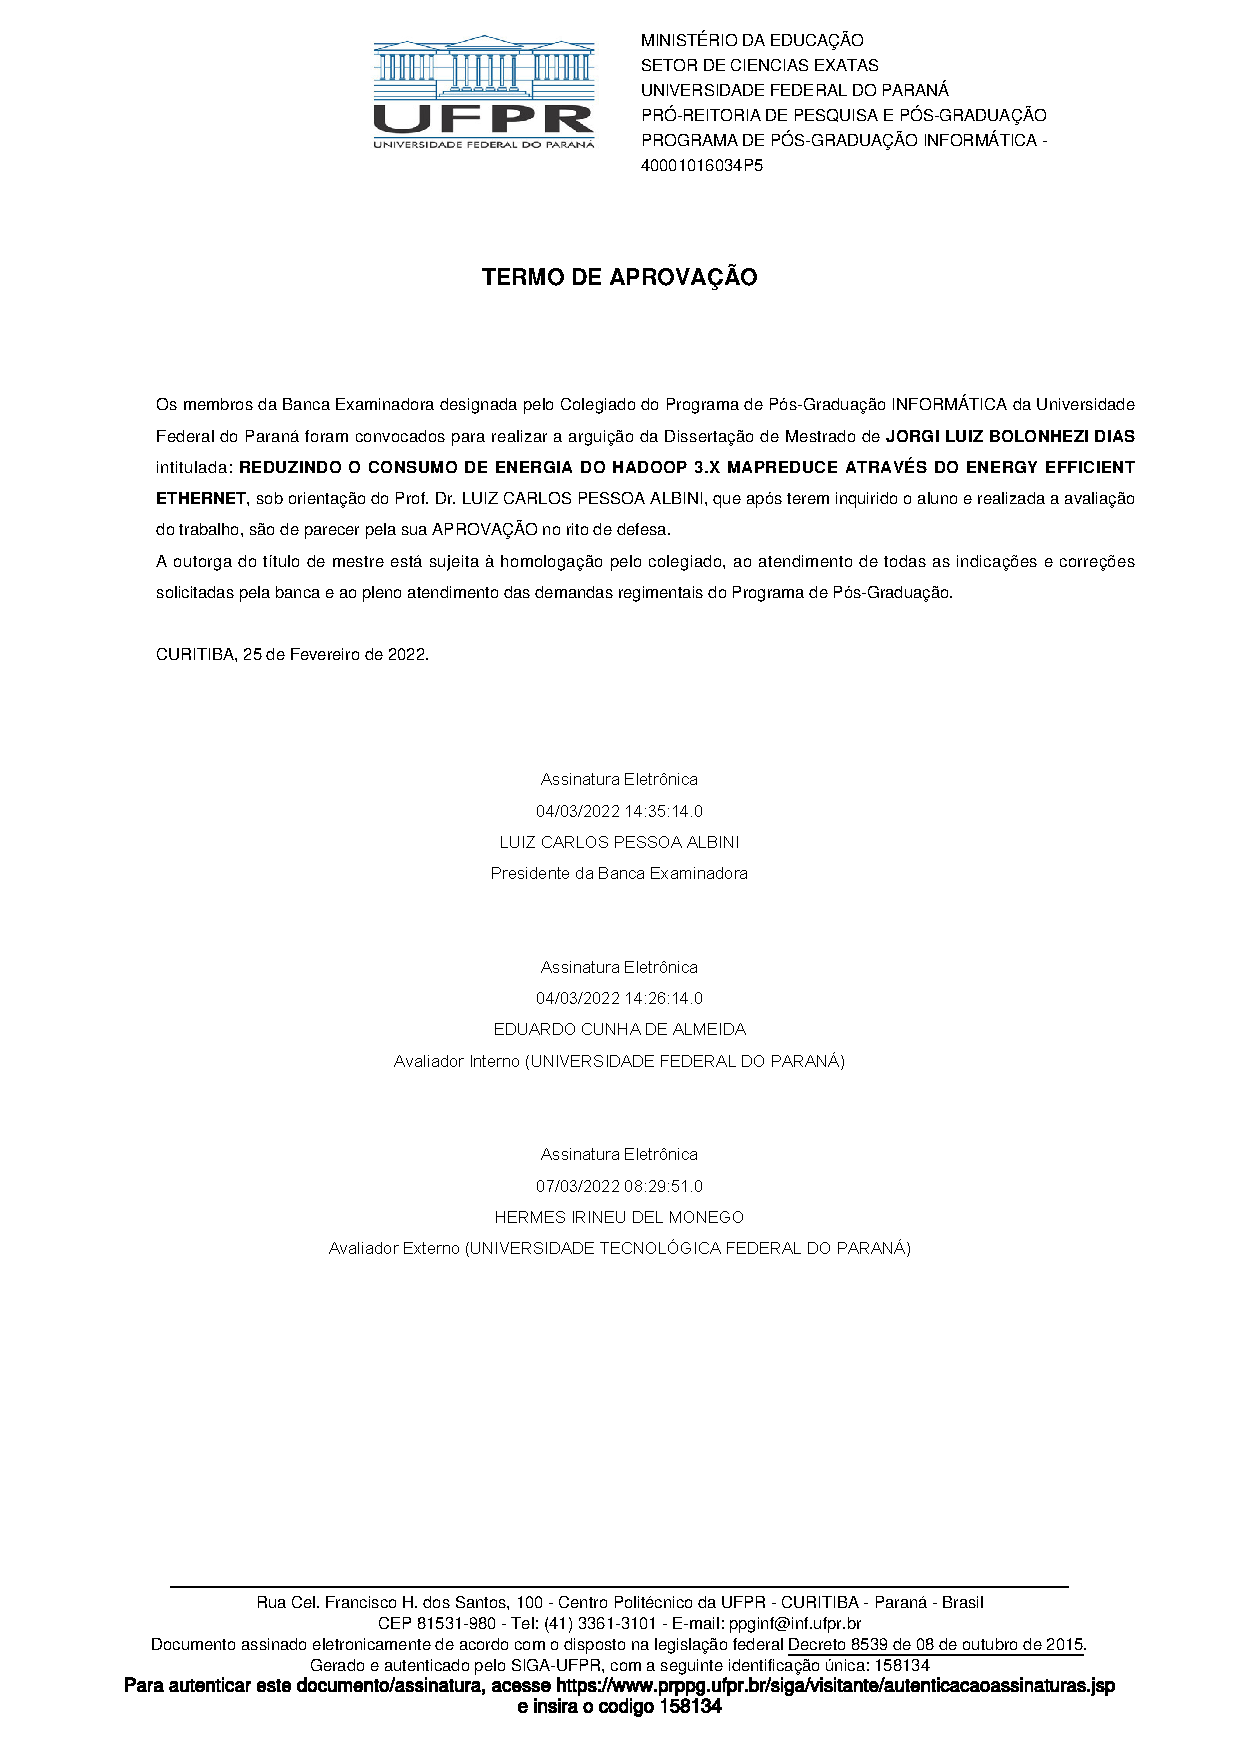
\includepdf[noautoscale]{0-iniciais/Aprovado.pdf}

\end{aprovacao}

%=====================================================
		% folha de aprovação
\begin{dedica}  % só gera conteúdo se for na versão final

A toda equipe da UFPR pela oportunidade de estudo.

\end{dedica}

		% dedicatória
\begin{agradece}	% só gera conteúdo se for na versão final

Agradeço a minha família, pelo apoio e incentivo nas horas difíceis. Aos professores, pelos ensinamentos e correções que me permitiram apresentar um melhor desempenho na minha formação profissional. Aos orientadores Luiz e Leandro, pelo seu grande desprendimento em ajudar e amizade sincera. Por fim, agradeço a todos que contribuíram diretamente ou indiretamente durante a formação.

\end{agradece}

		% agradecimentos

% resumo (português) e abstract (inglês)
\begin{resumo}

O consumo de energia é um dos maiores desafios na infraestrutura de processamento de \emph{Big Data}. Atualmente os gastos com energia são ainda maiores do que na aquisição do \emph{hardware}, representando 75\% do custo total dos \emph{data centers}. Aproximadamente 30\% de toda a energia do \emph{data center} é consumida por \emph{switches} de rede. O \emph{Energy Efficient Ethernet} é um padrão recente que visa reduzir o consumo de energia, embora a prática atual na indústria seja desativá-lo em produção, pois pode causar sobrecargas na rede e perda de desempenho. Esta dissertação fornece uma visão geral de como a atual versão do Apache Hadoop, a 3.x, se comporta com o \emph{Energy Efficient Ethernet} habilitado para links de 1GbE até 400GbE. Os resultados apresentados mostram que há economia de energia significativa com pouca ou nenhuma perda de desempenho para conexões de até 40GbE. No entanto, conexões de 100GbE e 400GbE apresentam perdas significativas de desempenho devido ao despertar do link para transmissões de um único \emph{frame}.



%Cada dia mais a produção de dados pela sociedade tem aumentado, o que implica em maior demanda de recursos e tecnologias viáveis para armazenar, processar e extrair informações úteis de todos estes dados. Uma das alternativas encontradas para tal tarefa foi a criação de \emph{clusters} Hadoop, que utilizam o \emph{framework MapReduce} e podem ser implementados com \emph{hardwares} de baixo custo. Entretanto, um outro problema permanece, o consumo massivo de energia em \emph{data centers}, que tem sido um assunto muito discutido recentemente pela comunidade e indústria. Algumas pesquisas foram realizadas buscando soluções para tal problema, como a criação do EEE-802.3az, um protocolo de rede conhecido como \emph{Green Ethernet}, e o E-EON - \emph{Energy-Efficient and Optimized Networks}, um conjunto de técnicas para redução do consumo de energia no Hadoop, diminuição da latência e aumento da taxa de transferência de rede. Esta pesquisa tem como objetivo principal avaliar e reduzir o consumo de energia da atual versão do Hadoop MapReduce, a 3.x, e para que isso seja alcançado, utilizaremos o NetSLS em testes de diversas configurações de rede sugeridas pelo E-EON como \emph{Ethernet Energy Efficient}, Coalescência de Pacotes e \emph{Active Queue Management}, buscando assim identificar a melhor combinação de rede possível para esta versão.

\end{resumo}
\begin{abstract}

Energy consumption is one of the major challenges on the big data processing infrastructure. The energy expenses are even higher than hardware, accounting for 75\% of the total cost of nowadays data centers. Narrowing, approximately 30\% of all data center energy is consumed by the network switches. Energy Efficient Ethernet is a recent standard aiming at reduce network power consumption, notwithstanding the current practice in industry is to disable it in production use, since it can cause network overloads and  performance loss. This thesis provides an overview on how Apache Hadoop 3.x, the current version, behaves with Energy Efficient Ethernet enabled for links from 1GbE up to 400GbE links. Presented results show that there is significant energy savings with little or no performance loss for connections up to 40GbE. Nevertheless, connections of 100GbE and 400GbE present significant performance losses due to link wake up to single transmissions.

%Everyday, the data production by society has increased, which results in a greater demand for viable resources and technologies to store, process and extract useful information from all these data. An alternative found for this task are the creation of Hadoop clusters, that uses the MapReduce framework and can be implemented on low cost hardware. However, there's another persistent problem, a massive energy consumption in data centers, which has been a subject much discussed recently by community and industry. Some research was carried out looking for solutions to this problem, such as the EEE-802.3az creation, a network protocol known as Green Ethernet, and Energy-Efficient and Optimized Networks, a techniques set for reducing energy consumption on Hadoop, decreased latency and increased network throughput. The main objective in this research are evaluate and reduce the energy consumption of the current version of Hadoop MapReduce, the 3.x, and for that to be achieved, we will use NetSLS in tests of various network configurations suggested by E-EON as Ethernet Energy Efficient, Packet Coalesing and Active Queue Management for try to identify the best possible network combination for this version. %

\end{abstract}

% listas  de figuras, tabelas, abreviações/siglas, símbolos
\listoffigures				% figuras
\clearpage
\listoftables				% tabelas
%=====================================================

% lista de acrônimos (siglas e abreviações)

\begin{listaacron}

\begin{longtable}[l]{p{0.2\linewidth}p{0.7\linewidth}}
ACK & \emph{Acknowledge}\\
API & \emph{Application Programming Interface}\\
AM & \emph{Application Master}\\
AQM & \emph{Active Queue Management}\\
CDN & \emph{Content Delivery Networks}\\
CE & \emph{Congestion Experienced}\\
CoDel & \emph{Controlled Delay}\\
CPU & \emph{Central Processing Unit}\\
CWR & \emph{Congestion Window Reduced}\\
EC & \emph{Erasure Coding}\\
ECN & \emph{Explicit Congestion Notification}\\
ECE & \emph{ECN-Echo}\\
ECT & \emph{ECN-Capable Transport}\\
EEE & \emph{Energy Efficient Ethernet}\\
E-EON & \emph{Energy-Efficient and Optimized Networks}\\
FIFO & \emph{First In First Out}\\
GC & \emph{Grid Computing}\\
GB & \emph{Gigabytes}\\
HDFS & \emph{Hadoop Distributed File System}\\
HPC & \emph{High-performance Computing}\\
IEEE &  \emph{Institute of Electrical and Electronics Engineers}\\
IP & \emph{Internet Protocol}\\
I/O & \emph{Imput and Ouput}\\
JVM & \emph{Java Virtual Machine}\\
KWh & Quilowatt-hora\\
LAN & \emph{Local Area Network}\\
LPI & \emph{Low Power Idle}\\
MADLFS & \emph{Microsoft Azure Data Lake File System}\\
MII & \emph{Media Independent Interface}\\
MRJ & \emph{MapReduce Job}\\
NM & \emph{Node Manager}\\
NIC & \emph{Network Interface Controller}\\
RAM & \emph{Random Access Memory}\\
RED & \emph{Random Early Detection}\\
RM & \emph{Resource Manager}\\
SAN & \emph{Storage Area Network}\\
SYN & \emph{Synchronize}\\
TCP & \emph{Transmission Control Protocol}\\
TWh & Terawatt-hora\\
WAN & \emph{Wide Área Network}\\
Wh & Watt-hora\\
YARN & \emph{Yet Another Resource Negotiator}\\
\end{longtable}

\end{listaacron}

%=====================================================
		% acrônimos, deve ser preenchida à mão
% %=====================================================

% lista de símbolos

\begin{listasimb}

\begin{longtable}[l]{p{0.2\linewidth}p{0.7\linewidth}}
% $\alpha$ & alfa, primeira letra do alfabeto grego\\
% $\beta$ & beta, segunda letra do alfabeto grego\\
% $\gamma$ & gama, terceira letra do alfabeto grego\\
%$\Omega$ & Ômega, última letra do alfabeto grego\\
µs & Microsegundos\\
% $\pi$ & pi \\
% $\tau$ & Tempo de resposta do sistema\\
% $\theta$ & Ângulo de incidência do raio luminoso\\
® & Marca Registrada no INPI\\
™ & Trade Mark\\
\end{longtable}

\end{listasimb}

%=====================================================
		% símbolos, idem
\tableofcontents			% sumário

%=====================================================

% define estilo do corpo do documento (capítulos e apêndices)
\mainmatter
\pagestyle{mainmatter}

% inclusao de cada capítulo, alterar a gosto (do professor de Metodologia)
\chapter{Energy Efficient Ethernet em Clusters Hadoop MapReduce}

Neste capítulo são apresentados os resultados das simulações de \emph{clusters Hadoop 3.x MapReduce} utilizando a ferramenta NetSLS e o \emph{Energy Efficient Ethernet} em modo \emph{Fast Wake} e \emph{Deep Sleep}. Através destes dados mostramos que uma boa economia de energia pode ser obtida em conexões de até 40GbE, enquanto conexões acima de 100GbE possuem problemas de performance quando o EEE está habilitado no modo \emph{Deep Sleep}.

\section{Economia de Energia}

Esta seção contém os dados de economia de energia obtidos das simulações com topologia \emph{leaf-spine} e conexões de 1GbE e 10GbE; 1GbE e 25GbE; 10GbE e 100GbE; 10GbE e 400GbE; 25GbE e 400GbE; e, finalmente, 40GbE e 400GbE. O restante da metodologia empregada pode ser visualizada no Capítulo 3 de forma detalhada.

\begin{figure}[htp]
    \centering
    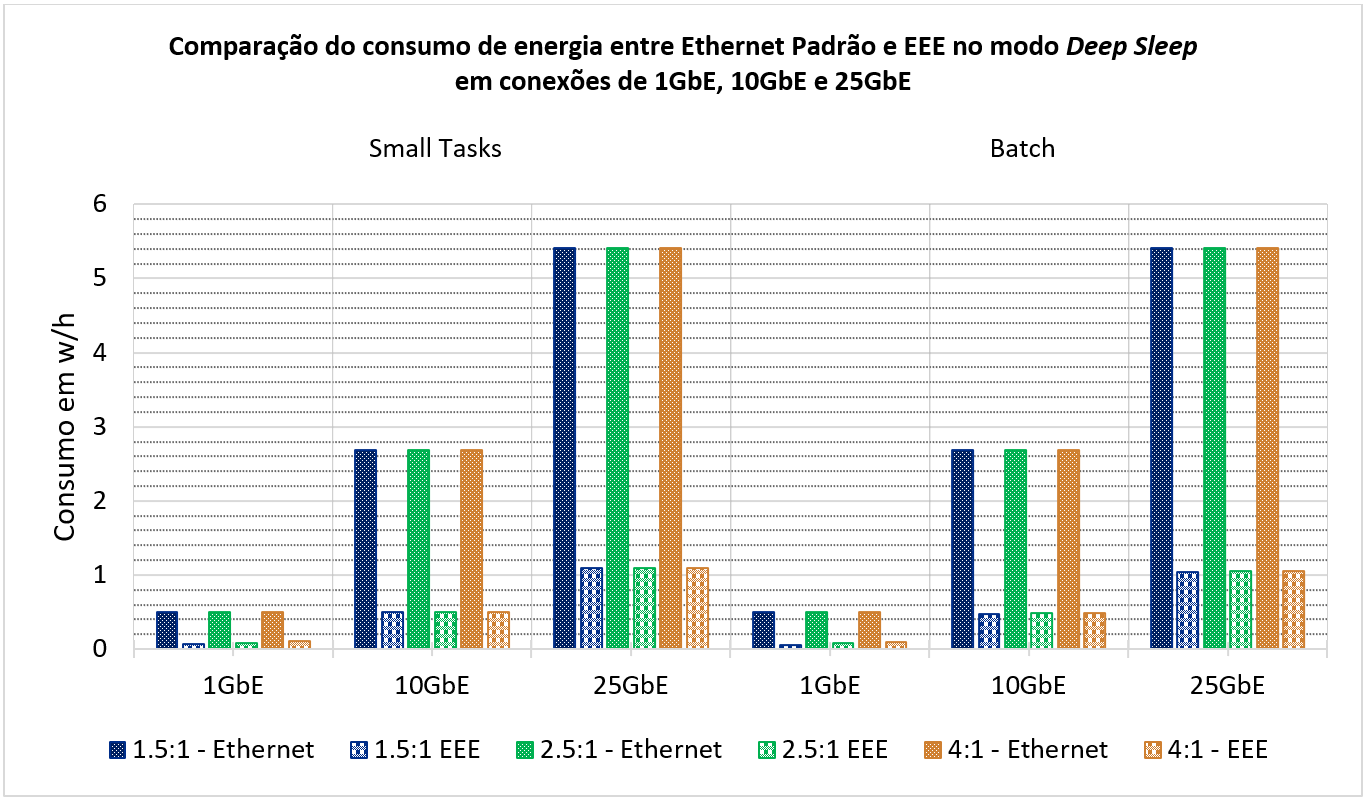
\includegraphics[width=16cm]{4-EEEHadoop/Image1_EEEConsumption1-10-25.PNG}
    \caption{\centering Comparação do consumo de energia entre \emph{Ethernet} Padrão e EEE no modo \emph{Deep Sleep} em conexões de 1GbE, 10GbE e 25GbE}
    \label{fig:EEEConsumption1-10-25}
\end{figure}

\begin{figure}[htp]
    \centering
    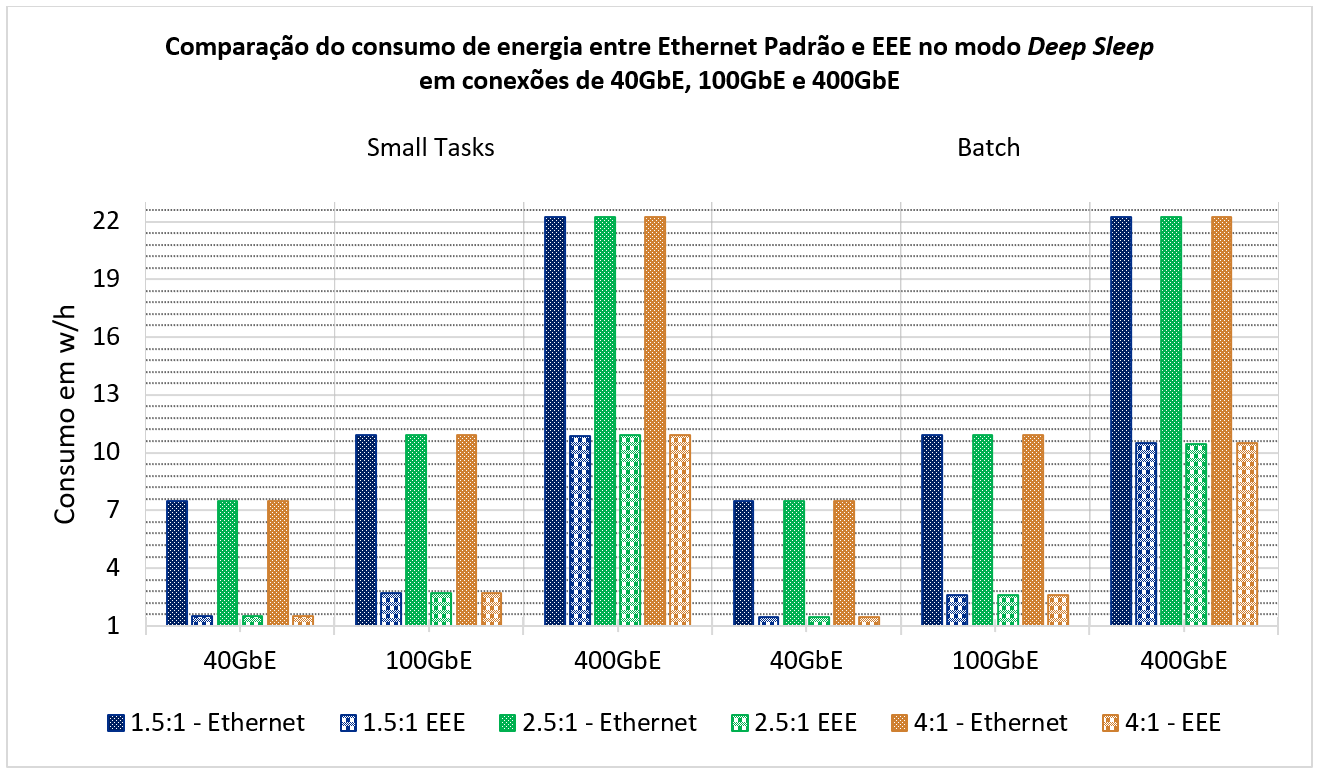
\includegraphics[width=16cm]{4-EEEHadoop/Image2_EEEConsumption40-100-400.PNG}
    \caption{\centering Comparação do consumo de energia entre \emph{Ethernet} Padrão e EEE no modo \emph{Deep Sleep} em conexões de 40GbE, 100GbE e 400GbE}
    \label{fig:EEEConsumption40-100-400}
\end{figure}

\begin{figure}[htp]
    \centering
    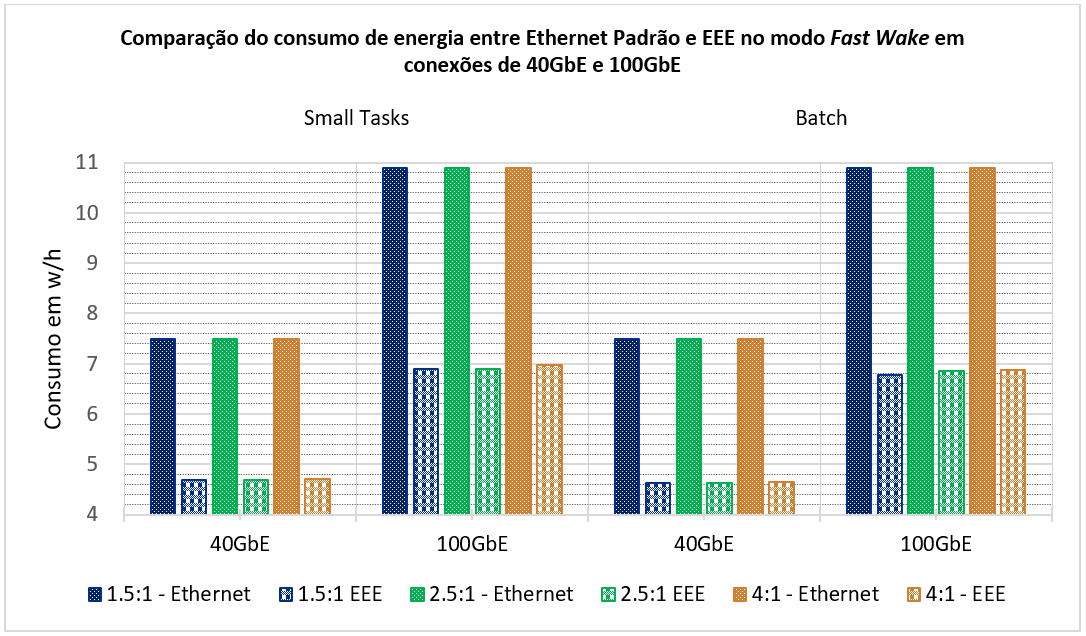
\includegraphics[width=16cm]{4-EEEHadoop/Image5_EEEConsumption40-100-FastWakeMode.PNG}
    \caption{\centering Comparação do consumo de energia entre \emph{Ethernet} Padrão e EEE no modo \emph{Fast Wake} em conexões de 40GbE e 100GbE}
    \label{fig:EEEConsumption100-400FastWakeMode}
\end{figure}

Através das simulações com o modo \textbf{\emph{Deep Sleep}} do EEE encontramos os dados mostrados nas figuras 4.1 e 4.2, que demonstram a economia de energia em \emph{Jobs MapReduce} em \emph{clusters}{} Hadoop 3.x, com reduções médias de 0,5w/h para 0,080w/h em links de 1GbE - redução de 83,89\%; 2,68w/h para 0,490w/h em 10GbE - redução de 81,68\%; de 5,41w/h para 1,072w/h em 25GbE - redução de 80,12\%; 7,49w/h para 1,487w/h em 40GbE - redução de 80,14\%; de 10,89w/h para 2,646w/h em 100GbE - redução de 75,69\%; e de 22,21w/h para 10,685w/h em 400GbE - redução de 51,89.

Usando a configuração de topologia de rede \emph{leaf-spine} recomendada pela Cisco, com uma taxa de assinatura excessiva igual a 4:1, encontramos resultados que, como em \cite{silva2018eon}; \cite{e2015exploring}; \cite{e2017energy}, apontam para economias de energia semelhantes habilitando o EEE no modo \textbf{\emph{Deep Sleep}} ao executar \emph{Small Tasks} e \emph{Batch Jobs}, no entanto, os \emph{Batch Jobs} tiveram um desempenho ligeiramente melhor.

Como pode-se observar na figura 4.3, ao habitarmos o EEE no modo \textbf{\emph{Fast Wake}} para as conexões de 40GbE e 100GbE, percebe-se uma economia de energia relativamente menor do que comparado ao modo \textbf{\emph{Deep Sleep}}, de 7,49w/h para 4,634w/h em conexões de 40GbE - redução de 38,13\%, e de 10,89w/h para 6,916w/h - redução de 36,49\% em conexões de 100GbE respectivamente. Em contrapartida, o desempenho foi melhor como detalhado na próxima seção.

\section{Desempenho}

Esta seção contém os dados de performance obtidos das simulações com topologia \emph{leaf-spine} e conexões de 1GbE e 10GbE; 1GbE e 25GbE; 10GbE e 100GbE; 10GbE e 400GbE; 25GbE e 400GbE; e, finalmente, 40GbE e 400GbE. O restante da metodologia empregada pode ser visualizada no Capítulo 3 de forma detalhada.

Ao contrário do que afirmam os fornecedores de equipamentos, nossos testes demonstram que é possível obter uma boa economia de energia habilitando o \emph{Energy Efficient Ethernet} no modo \textbf{\emph{Deep Sleep}}, com uma perda média de desempenho de praticamente zero para links de 1GbE - 0,21\%; 10GbE - 0,94\%; e 25GbE - 1,52\%; ou razoável no caso de 40GbE - 2,85\% conforme mostrado nas figuras 4.4 e 4.5. Para links de 100GbE e 400GbE há uma boa economia de energia, mas com uma perda de desempenho que não é considerada ideal, em torno de 4,55\% e 8,58\% respectivamente.

Em geral, ao habilitar o EEE em modo \textbf{\emph{Deep Sleep}} no \emph{cluster}, percebe-se que os \emph{Batch Jobs} obtêm melhor economia de energia e desempenho em relação aos \emph{Small Tasks}. Ainda é possível observar um cenário específico, em que ao diminuir a taxa de assinatura excessiva da rede para 1.5:1 em links 1GbE, os \emph{Batch Jobs} obtiveram uma melhora significativamente maior na economia de energia e no desempenho em comparação com outras conexões.

\begin{figure}[htp]
    \centering
    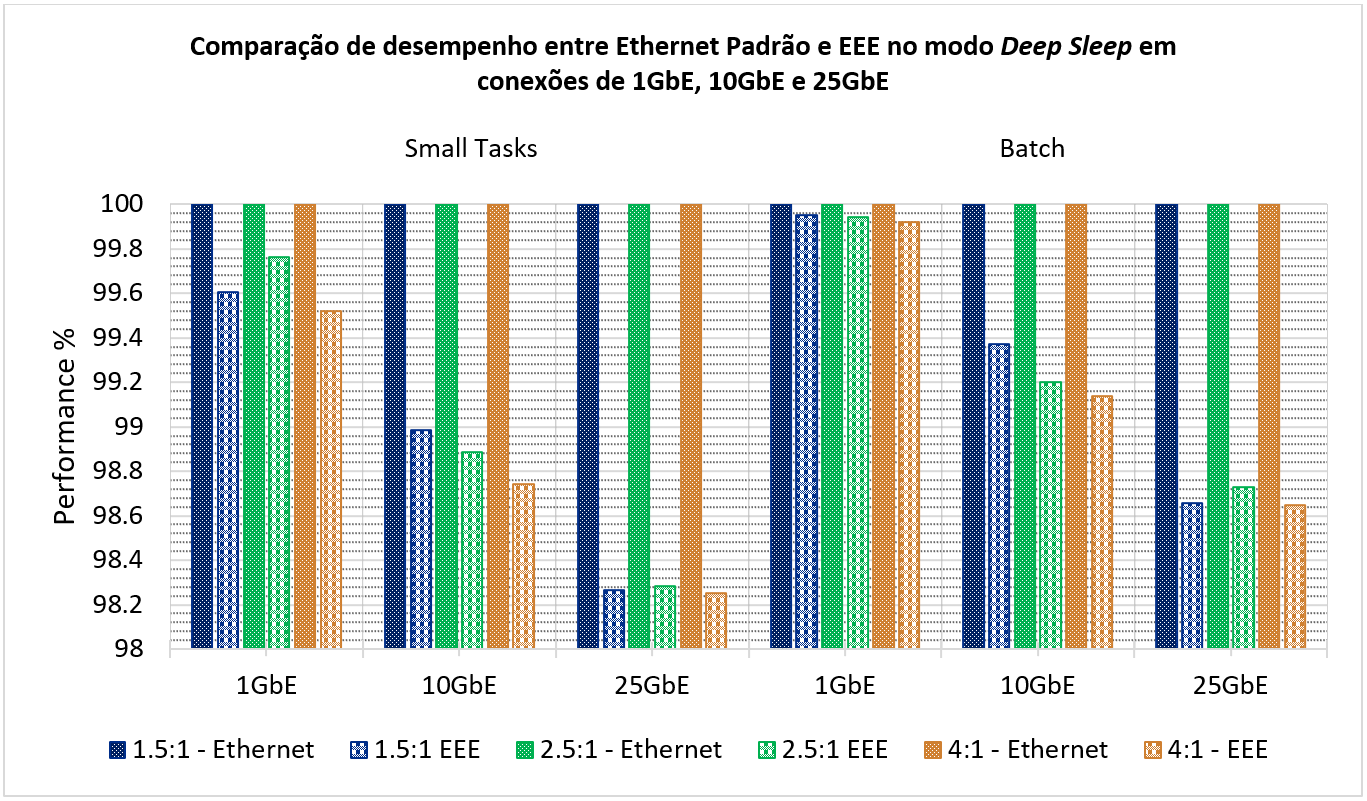
\includegraphics[width=16cm]{4-EEEHadoop/Image3_EEEPerformance1-10-25.PNG}
    \caption{\centering Comparação de desempenho entre \emph{Ethernet} Padrão e EEE no modo \emph{Deep Sleep} em conexões de 1GbE, 10GbE e 25GbE}
    \label{fig:EEEPerformance1-10-25}
\end{figure}

\begin{figure}[htp]
    \centering
    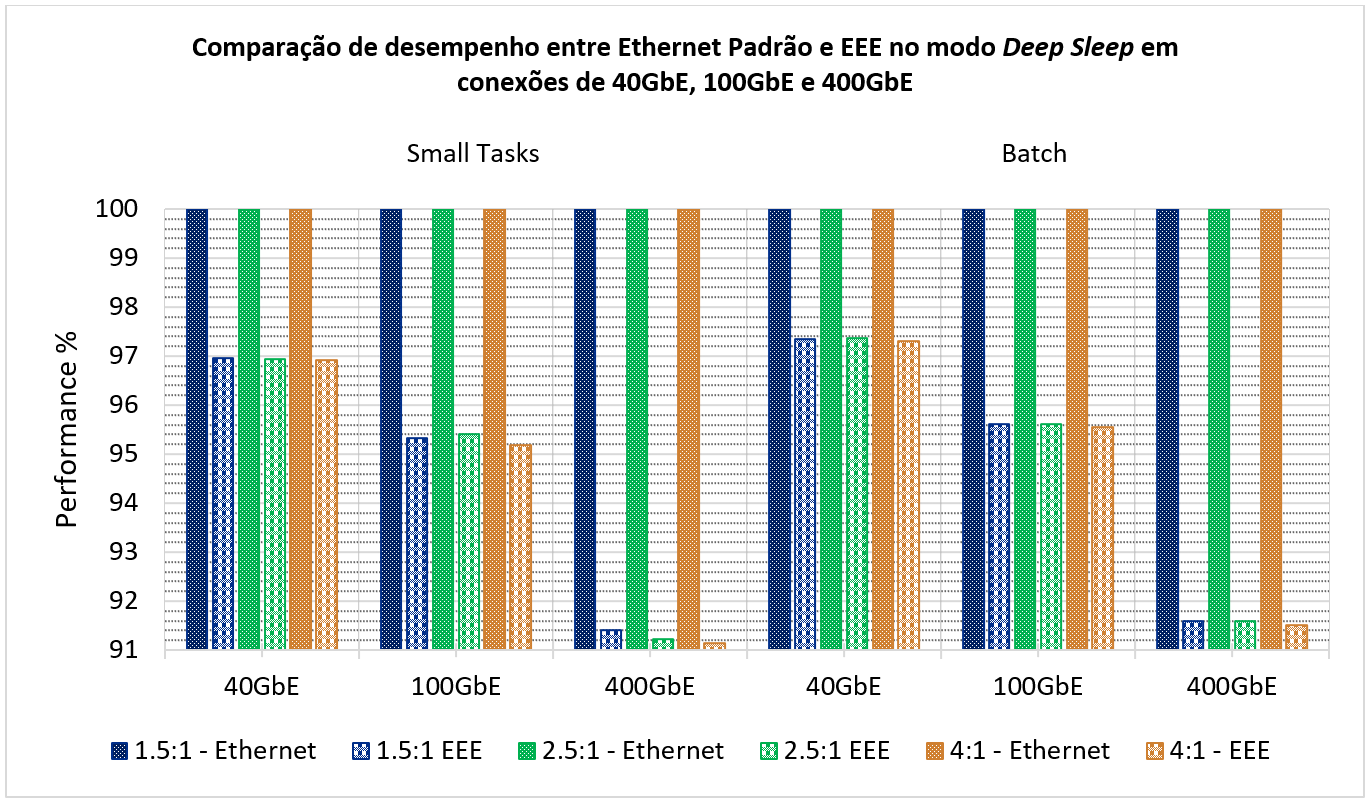
\includegraphics[width=16cm]{4-EEEHadoop/Image4_EEEPerformance40-100-400.PNG}
    \caption{\centering Comparação de desempenho entre \emph{Ethernet} Padrão e EEE no modo \emph{Deep Sleep} em conexões de 40GbE, 100GbE e 400GbE}
    \label{fig:EEEPerformance40-100-400}
\end{figure}

\begin{figure}[htp]
    \centering
    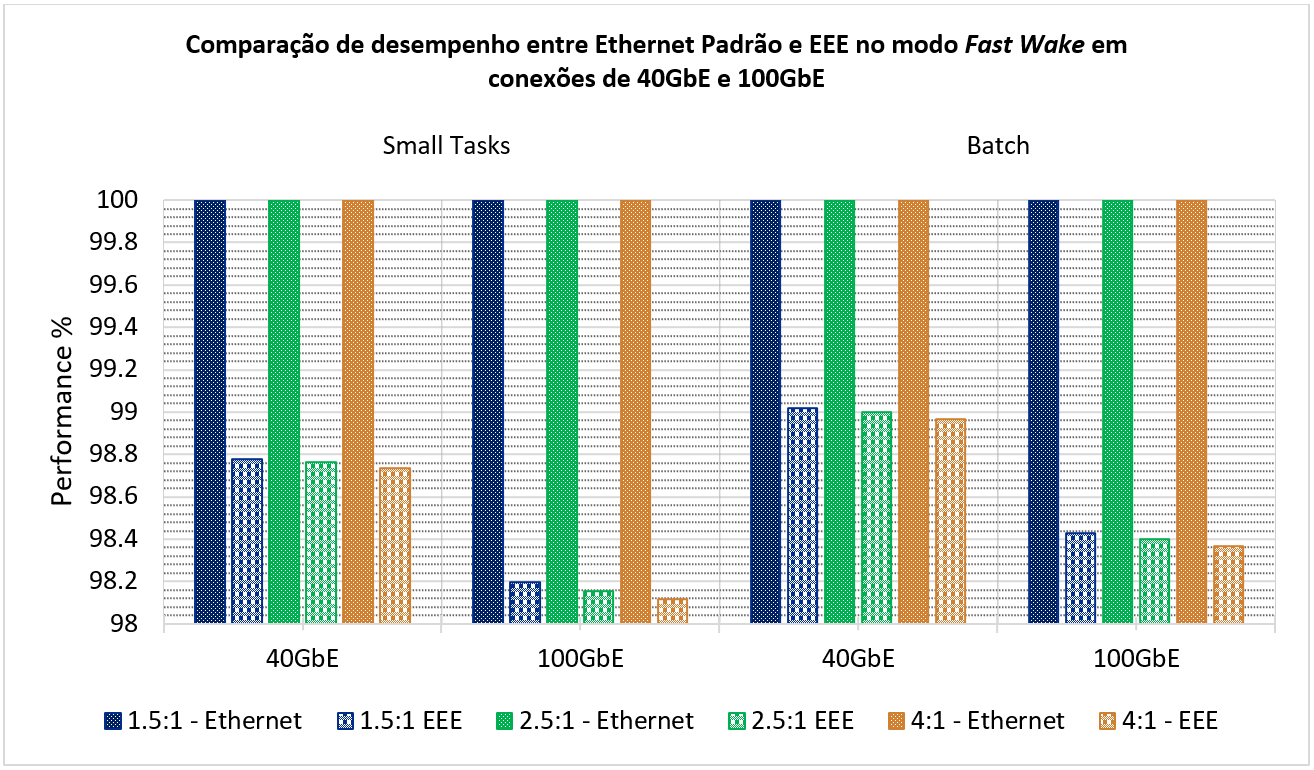
\includegraphics[width=16cm]{4-EEEHadoop/Image6_EEEPerformance40-100-FastWakeMode.PNG}
    \caption{\centering Comparação de desempenho entre \emph{Ethernet} Padrão e EEE no modo \emph{Fast Wake} em conexões de 40GbE e 100GbE}
    \label{fig:EEEPerformance40-100FastWake}
\end{figure}

Ao utilizarmos o modo \textbf{\emph{Fast Wake}} do EEE em nossas simulações, foi possível notar que embora este modo não forneça uma economia de energia como o modo \textbf{\emph{Deep Sleep}}, ele não afeta o desempenho de forma que seja considerável, com uma perda de 1,2\% no caso das conexões de 40GbE e 1,8\% em conexões de 100GbE, tornando-se assim uma opção interessante para as indústrias que buscam um balanceamento entre economia de energia e desempenho.  

As perdas de desempenho mais significativas encontradas para os links de 100GbE e 400GbE com o modo \textbf{\emph{Deep Sleep}} ocorreram porque em determinados momentos é necessário acordar um link para transmitir um único \emph{frame}, o que causa penalidades de latência e consumo de energia em termos relativos que são agravadas de acordo com a largura de banda \cite{jiang2021modeling}; \cite{reviriego2009performance}; \cite{reviriego2010burst}; \cite{e2017energy}. Se os momentos de \emph{wake} do EEE puderem ser controlados para evitar transmissões de um \emph{frame} único, pode ser possível obter economia de energia com perdas de desempenho baixas ou nulas para estas conexões.

\section{Considerações Finais}

Neste capítulo, apresentamos uma análise do impacto ao habilitar ao \emph{Energy Efficient Ethernet} nos modos \textbf{\emph{Deep Sleep}} e \textbf{\emph{Fast Wake}} em \emph{clusters MapReduce} que utilizam o \emph{framework} Apache Hadoop 3.x. Avaliamos execuções de \emph{Small Tasks} e \emph{Batch Jobs} com EEE em diversos \emph{clusters} simulados, e no modo \textbf{\emph{Deep Sleep}} encontramos economia de energia entre 78\% e 82\% para links de até 40GbE sem perda considerável de desempenho, entre 0,21\% e 2,85 \%. Para links de 100GbE e 400GbE houve uma economia de energia significativa de 75,69\% e 51,88\% respectivamente, mas com uma taxa de perda de desempenho considerável de 4,55\% e 8,58\%, o que não é particularmente interessante em \emph{Batch Jobs}. Quando optamos pelo uso do modo \textbf{\emph{Fast Wake}} do EEE, obtivemos uma redução do consumo de 7,49w/h para 4,634w/h em conexões de 40GbE, e de 10,89w/h para 6,916w/h em conexões de 100GbE, com uma perda de performance de 1.2\% e 1.8\%.

Em termos de custo-benefício para \emph{data centers}, o recomendado para conexões de até 40GbE é habilitar o EEE no modo \textbf{\emph{Deep Sleep}}, o que resulta em uma boa redução do consumo de energia e uma taxa de perda de desempenho baixa ou nula. Para conexões de 100GbE o recomendado é habilitar o modo \textbf{\emph{Fast Wake}} do EEE, obtendo assim um balanceamento entre consumo de energia e performance. Para conexões de 400GbE habilitar o EEE não é interessante, pois há uma perda de 8,58\% do desempenho.

O problema de latência e economia de energia encontrado em conexões acima de 100GbE com \textbf{\emph{Deep Sleep}} são causados por ter que acordar o link de tempos em tempos para transmitir um único \emph{frame}. Para resolver este problema, no próximo capítulo combinamos o \emph{Energy Efficient Ethernet} com \emph{Packet Coalescing}, \emph{Random Early Detection}, \emph{Controlled Delay}  e \emph{Explicit Congestion Notification}, podendo assim configurar de forma manual e inteligente quando os links devem ser acordados do modo LPI para transmissões de pacotes.

			% introdução
\chapter{Energy Efficient Ethernet em Clusters Hadoop MapReduce}

Neste capítulo são apresentados os resultados das simulações de \emph{clusters Hadoop 3.x MapReduce} utilizando a ferramenta NetSLS e o \emph{Energy Efficient Ethernet} em modo \emph{Fast Wake} e \emph{Deep Sleep}. Através destes dados mostramos que uma boa economia de energia pode ser obtida em conexões de até 40GbE, enquanto conexões acima de 100GbE possuem problemas de performance quando o EEE está habilitado no modo \emph{Deep Sleep}.

\section{Economia de Energia}

Esta seção contém os dados de economia de energia obtidos das simulações com topologia \emph{leaf-spine} e conexões de 1GbE e 10GbE; 1GbE e 25GbE; 10GbE e 100GbE; 10GbE e 400GbE; 25GbE e 400GbE; e, finalmente, 40GbE e 400GbE. O restante da metodologia empregada pode ser visualizada no Capítulo 3 de forma detalhada.

\begin{figure}[htp]
    \centering
    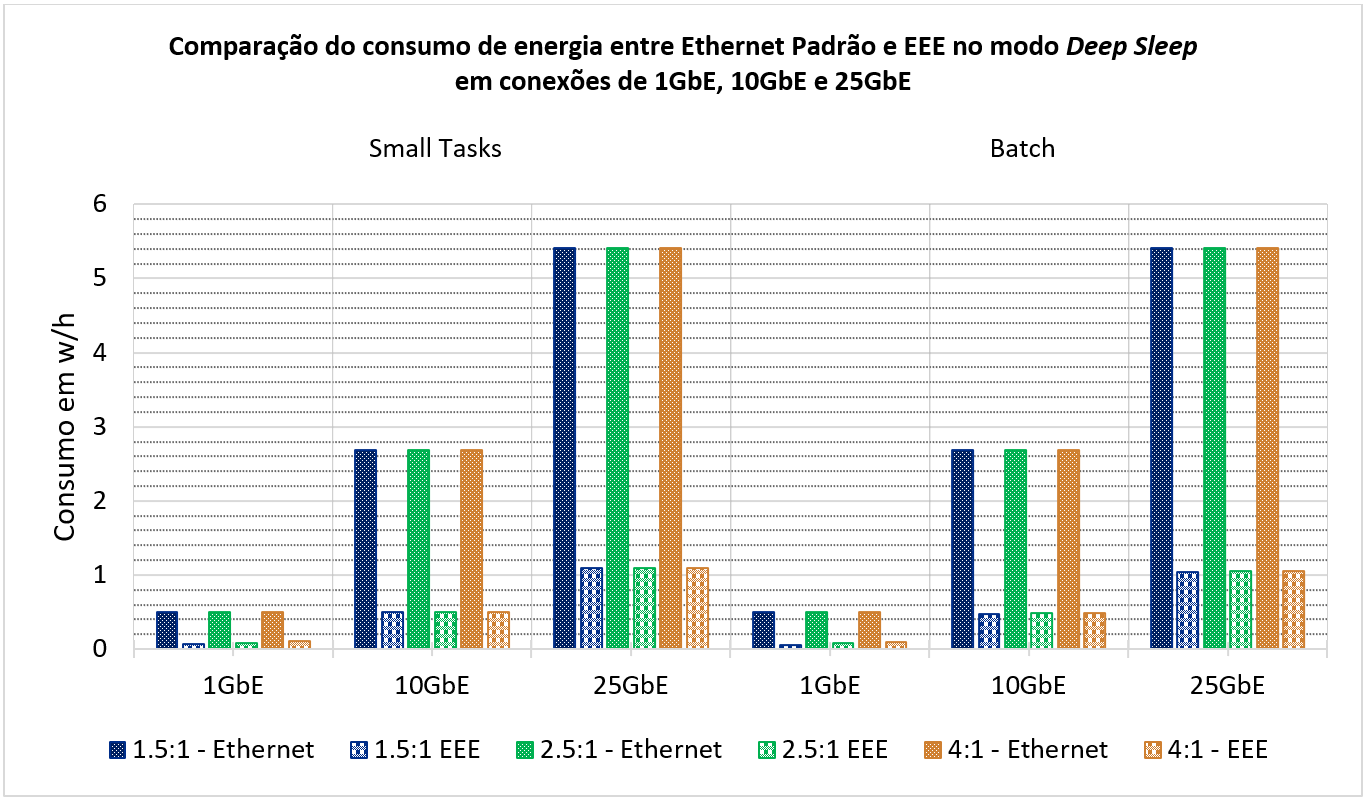
\includegraphics[width=16cm]{4-EEEHadoop/Image1_EEEConsumption1-10-25.PNG}
    \caption{\centering Comparação do consumo de energia entre \emph{Ethernet} Padrão e EEE no modo \emph{Deep Sleep} em conexões de 1GbE, 10GbE e 25GbE}
    \label{fig:EEEConsumption1-10-25}
\end{figure}

\begin{figure}[htp]
    \centering
    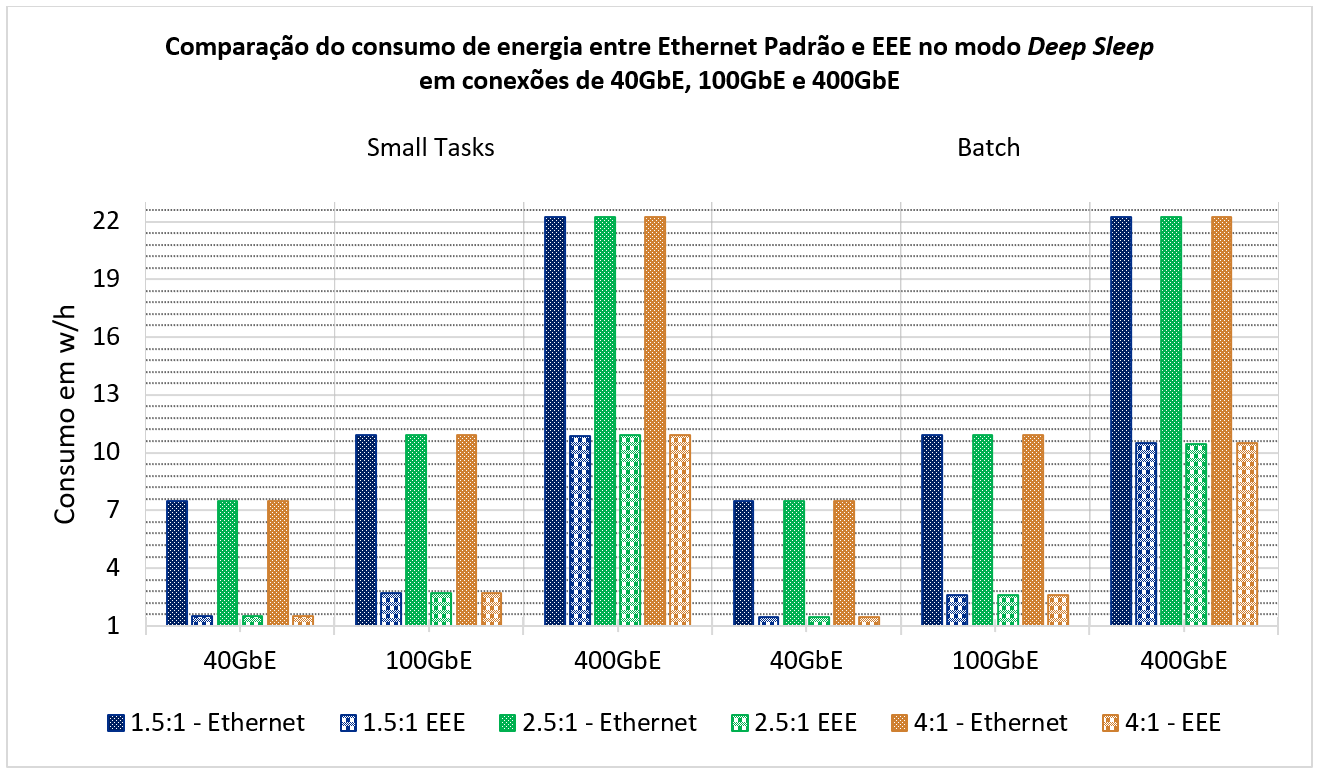
\includegraphics[width=16cm]{4-EEEHadoop/Image2_EEEConsumption40-100-400.PNG}
    \caption{\centering Comparação do consumo de energia entre \emph{Ethernet} Padrão e EEE no modo \emph{Deep Sleep} em conexões de 40GbE, 100GbE e 400GbE}
    \label{fig:EEEConsumption40-100-400}
\end{figure}

\begin{figure}[htp]
    \centering
    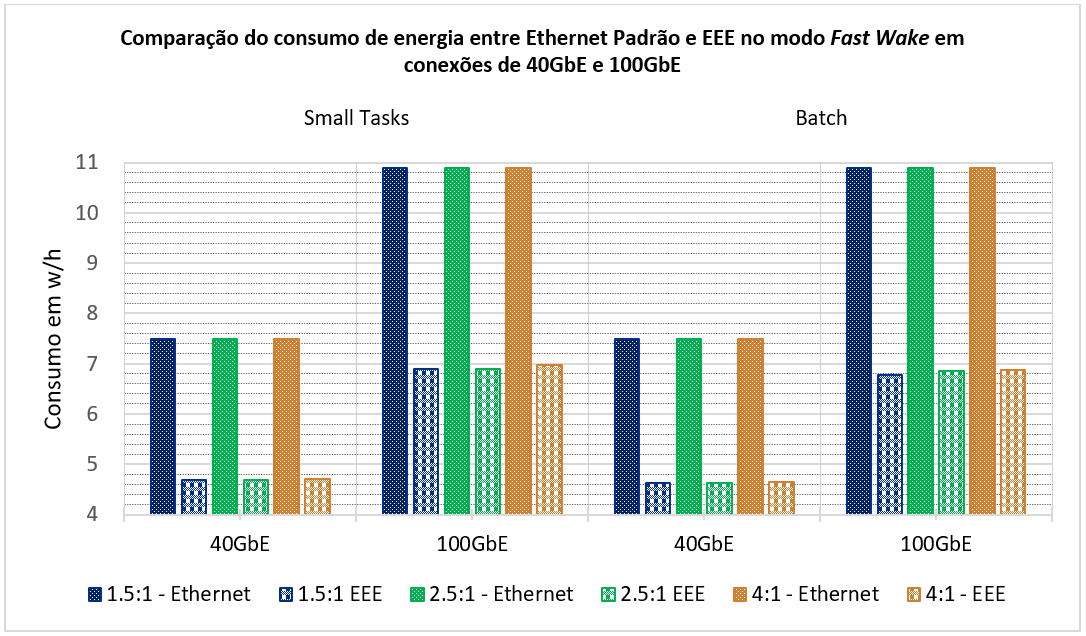
\includegraphics[width=16cm]{4-EEEHadoop/Image5_EEEConsumption40-100-FastWakeMode.PNG}
    \caption{\centering Comparação do consumo de energia entre \emph{Ethernet} Padrão e EEE no modo \emph{Fast Wake} em conexões de 40GbE e 100GbE}
    \label{fig:EEEConsumption100-400FastWakeMode}
\end{figure}

Através das simulações com o modo \textbf{\emph{Deep Sleep}} do EEE encontramos os dados mostrados nas figuras 4.1 e 4.2, que demonstram a economia de energia em \emph{Jobs MapReduce} em \emph{clusters}{} Hadoop 3.x, com reduções médias de 0,5w/h para 0,080w/h em links de 1GbE - redução de 83,89\%; 2,68w/h para 0,490w/h em 10GbE - redução de 81,68\%; de 5,41w/h para 1,072w/h em 25GbE - redução de 80,12\%; 7,49w/h para 1,487w/h em 40GbE - redução de 80,14\%; de 10,89w/h para 2,646w/h em 100GbE - redução de 75,69\%; e de 22,21w/h para 10,685w/h em 400GbE - redução de 51,89.

Usando a configuração de topologia de rede \emph{leaf-spine} recomendada pela Cisco, com uma taxa de assinatura excessiva igual a 4:1, encontramos resultados que, como em \cite{silva2018eon}; \cite{e2015exploring}; \cite{e2017energy}, apontam para economias de energia semelhantes habilitando o EEE no modo \textbf{\emph{Deep Sleep}} ao executar \emph{Small Tasks} e \emph{Batch Jobs}, no entanto, os \emph{Batch Jobs} tiveram um desempenho ligeiramente melhor.

Como pode-se observar na figura 4.3, ao habitarmos o EEE no modo \textbf{\emph{Fast Wake}} para as conexões de 40GbE e 100GbE, percebe-se uma economia de energia relativamente menor do que comparado ao modo \textbf{\emph{Deep Sleep}}, de 7,49w/h para 4,634w/h em conexões de 40GbE - redução de 38,13\%, e de 10,89w/h para 6,916w/h - redução de 36,49\% em conexões de 100GbE respectivamente. Em contrapartida, o desempenho foi melhor como detalhado na próxima seção.

\section{Desempenho}

Esta seção contém os dados de performance obtidos das simulações com topologia \emph{leaf-spine} e conexões de 1GbE e 10GbE; 1GbE e 25GbE; 10GbE e 100GbE; 10GbE e 400GbE; 25GbE e 400GbE; e, finalmente, 40GbE e 400GbE. O restante da metodologia empregada pode ser visualizada no Capítulo 3 de forma detalhada.

Ao contrário do que afirmam os fornecedores de equipamentos, nossos testes demonstram que é possível obter uma boa economia de energia habilitando o \emph{Energy Efficient Ethernet} no modo \textbf{\emph{Deep Sleep}}, com uma perda média de desempenho de praticamente zero para links de 1GbE - 0,21\%; 10GbE - 0,94\%; e 25GbE - 1,52\%; ou razoável no caso de 40GbE - 2,85\% conforme mostrado nas figuras 4.4 e 4.5. Para links de 100GbE e 400GbE há uma boa economia de energia, mas com uma perda de desempenho que não é considerada ideal, em torno de 4,55\% e 8,58\% respectivamente.

Em geral, ao habilitar o EEE em modo \textbf{\emph{Deep Sleep}} no \emph{cluster}, percebe-se que os \emph{Batch Jobs} obtêm melhor economia de energia e desempenho em relação aos \emph{Small Tasks}. Ainda é possível observar um cenário específico, em que ao diminuir a taxa de assinatura excessiva da rede para 1.5:1 em links 1GbE, os \emph{Batch Jobs} obtiveram uma melhora significativamente maior na economia de energia e no desempenho em comparação com outras conexões.

\begin{figure}[htp]
    \centering
    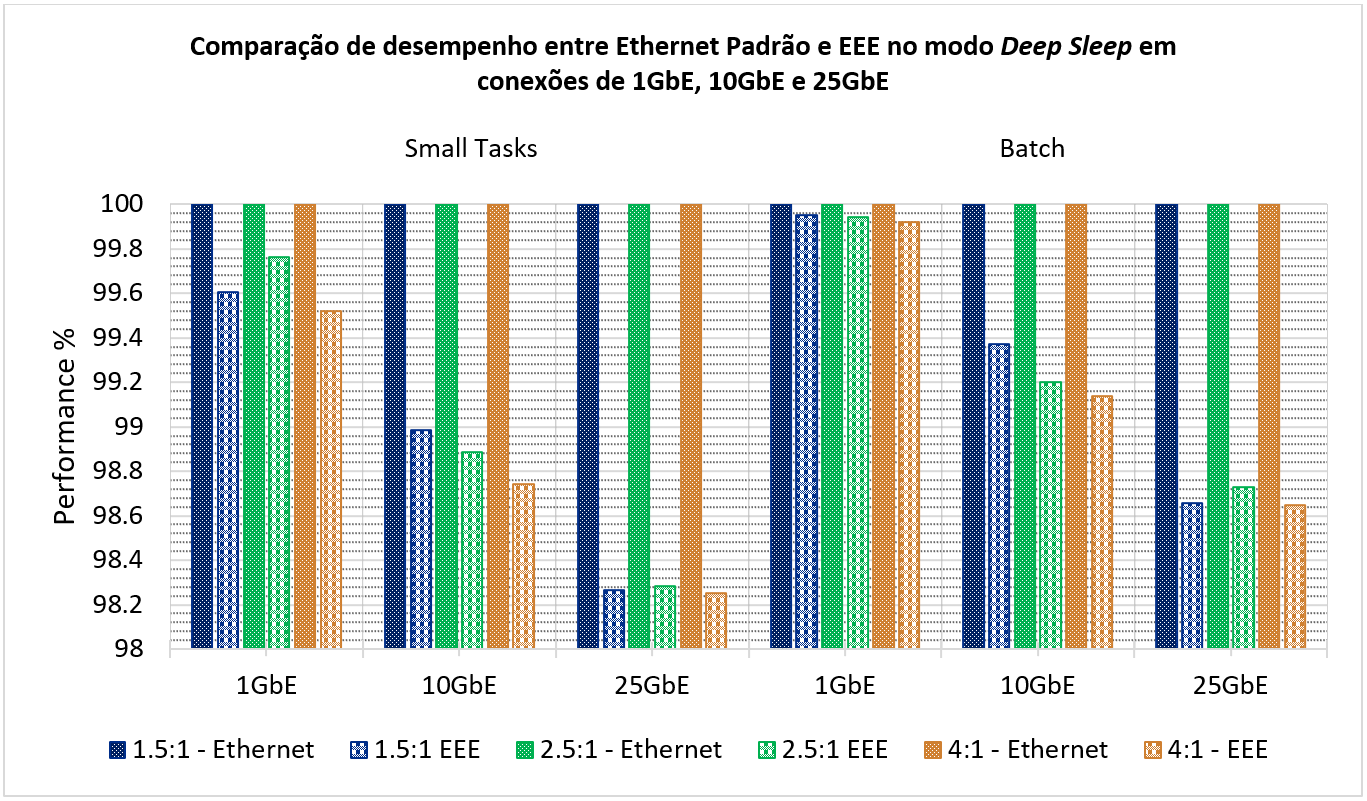
\includegraphics[width=16cm]{4-EEEHadoop/Image3_EEEPerformance1-10-25.PNG}
    \caption{\centering Comparação de desempenho entre \emph{Ethernet} Padrão e EEE no modo \emph{Deep Sleep} em conexões de 1GbE, 10GbE e 25GbE}
    \label{fig:EEEPerformance1-10-25}
\end{figure}

\begin{figure}[htp]
    \centering
    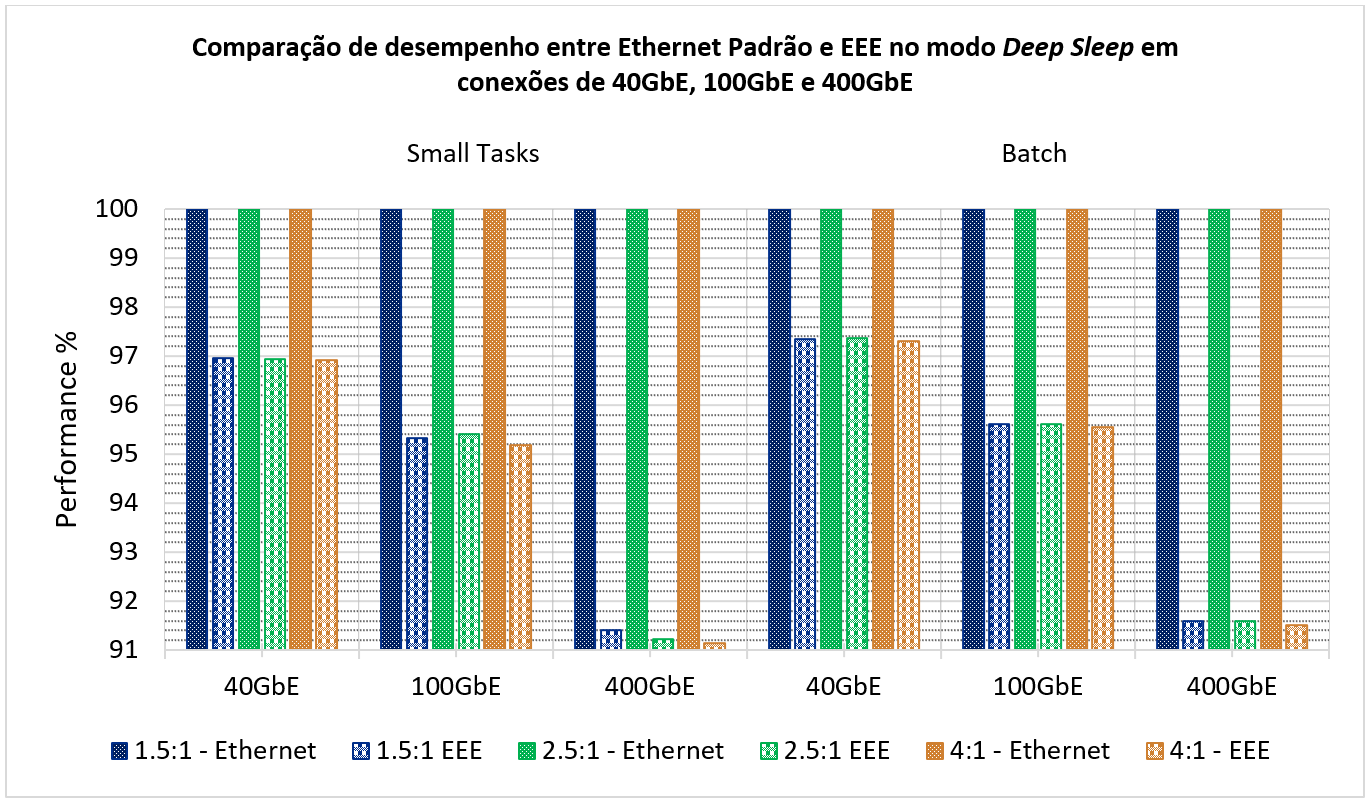
\includegraphics[width=16cm]{4-EEEHadoop/Image4_EEEPerformance40-100-400.PNG}
    \caption{\centering Comparação de desempenho entre \emph{Ethernet} Padrão e EEE no modo \emph{Deep Sleep} em conexões de 40GbE, 100GbE e 400GbE}
    \label{fig:EEEPerformance40-100-400}
\end{figure}

\begin{figure}[htp]
    \centering
    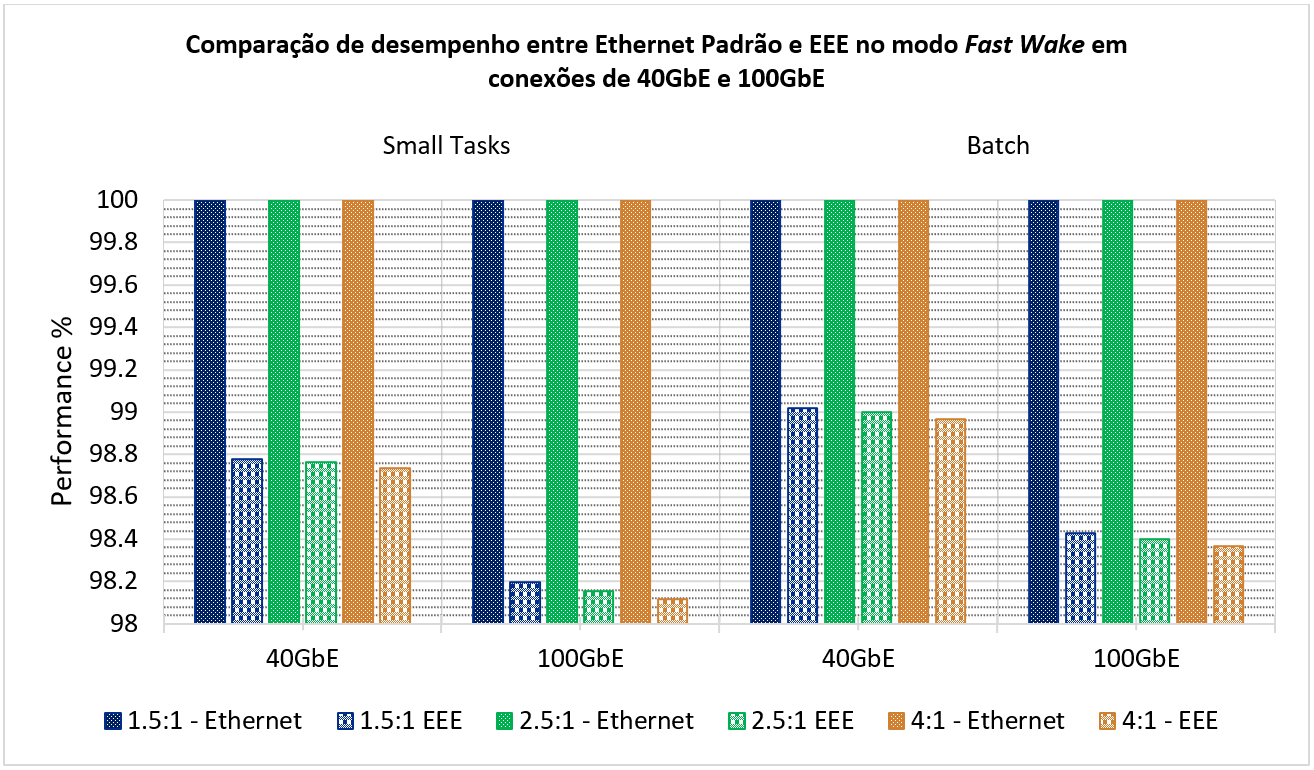
\includegraphics[width=16cm]{4-EEEHadoop/Image6_EEEPerformance40-100-FastWakeMode.PNG}
    \caption{\centering Comparação de desempenho entre \emph{Ethernet} Padrão e EEE no modo \emph{Fast Wake} em conexões de 40GbE e 100GbE}
    \label{fig:EEEPerformance40-100FastWake}
\end{figure}

Ao utilizarmos o modo \textbf{\emph{Fast Wake}} do EEE em nossas simulações, foi possível notar que embora este modo não forneça uma economia de energia como o modo \textbf{\emph{Deep Sleep}}, ele não afeta o desempenho de forma que seja considerável, com uma perda de 1,2\% no caso das conexões de 40GbE e 1,8\% em conexões de 100GbE, tornando-se assim uma opção interessante para as indústrias que buscam um balanceamento entre economia de energia e desempenho.  

As perdas de desempenho mais significativas encontradas para os links de 100GbE e 400GbE com o modo \textbf{\emph{Deep Sleep}} ocorreram porque em determinados momentos é necessário acordar um link para transmitir um único \emph{frame}, o que causa penalidades de latência e consumo de energia em termos relativos que são agravadas de acordo com a largura de banda \cite{jiang2021modeling}; \cite{reviriego2009performance}; \cite{reviriego2010burst}; \cite{e2017energy}. Se os momentos de \emph{wake} do EEE puderem ser controlados para evitar transmissões de um \emph{frame} único, pode ser possível obter economia de energia com perdas de desempenho baixas ou nulas para estas conexões.

\section{Considerações Finais}

Neste capítulo, apresentamos uma análise do impacto ao habilitar ao \emph{Energy Efficient Ethernet} nos modos \textbf{\emph{Deep Sleep}} e \textbf{\emph{Fast Wake}} em \emph{clusters MapReduce} que utilizam o \emph{framework} Apache Hadoop 3.x. Avaliamos execuções de \emph{Small Tasks} e \emph{Batch Jobs} com EEE em diversos \emph{clusters} simulados, e no modo \textbf{\emph{Deep Sleep}} encontramos economia de energia entre 78\% e 82\% para links de até 40GbE sem perda considerável de desempenho, entre 0,21\% e 2,85 \%. Para links de 100GbE e 400GbE houve uma economia de energia significativa de 75,69\% e 51,88\% respectivamente, mas com uma taxa de perda de desempenho considerável de 4,55\% e 8,58\%, o que não é particularmente interessante em \emph{Batch Jobs}. Quando optamos pelo uso do modo \textbf{\emph{Fast Wake}} do EEE, obtivemos uma redução do consumo de 7,49w/h para 4,634w/h em conexões de 40GbE, e de 10,89w/h para 6,916w/h em conexões de 100GbE, com uma perda de performance de 1.2\% e 1.8\%.

Em termos de custo-benefício para \emph{data centers}, o recomendado para conexões de até 40GbE é habilitar o EEE no modo \textbf{\emph{Deep Sleep}}, o que resulta em uma boa redução do consumo de energia e uma taxa de perda de desempenho baixa ou nula. Para conexões de 100GbE o recomendado é habilitar o modo \textbf{\emph{Fast Wake}} do EEE, obtendo assim um balanceamento entre consumo de energia e performance. Para conexões de 400GbE habilitar o EEE não é interessante, pois há uma perda de 8,58\% do desempenho.

O problema de latência e economia de energia encontrado em conexões acima de 100GbE com \textbf{\emph{Deep Sleep}} são causados por ter que acordar o link de tempos em tempos para transmitir um único \emph{frame}. Para resolver este problema, no próximo capítulo combinamos o \emph{Energy Efficient Ethernet} com \emph{Packet Coalescing}, \emph{Random Early Detection}, \emph{Controlled Delay}  e \emph{Explicit Congestion Notification}, podendo assim configurar de forma manual e inteligente quando os links devem ser acordados do modo LPI para transmissões de pacotes.

		% fundamentação teórica
\chapter{Energy Efficient Ethernet em Clusters Hadoop MapReduce}

Neste capítulo são apresentados os resultados das simulações de \emph{clusters Hadoop 3.x MapReduce} utilizando a ferramenta NetSLS e o \emph{Energy Efficient Ethernet} em modo \emph{Fast Wake} e \emph{Deep Sleep}. Através destes dados mostramos que uma boa economia de energia pode ser obtida em conexões de até 40GbE, enquanto conexões acima de 100GbE possuem problemas de performance quando o EEE está habilitado no modo \emph{Deep Sleep}.

\section{Economia de Energia}

Esta seção contém os dados de economia de energia obtidos das simulações com topologia \emph{leaf-spine} e conexões de 1GbE e 10GbE; 1GbE e 25GbE; 10GbE e 100GbE; 10GbE e 400GbE; 25GbE e 400GbE; e, finalmente, 40GbE e 400GbE. O restante da metodologia empregada pode ser visualizada no Capítulo 3 de forma detalhada.

\begin{figure}[htp]
    \centering
    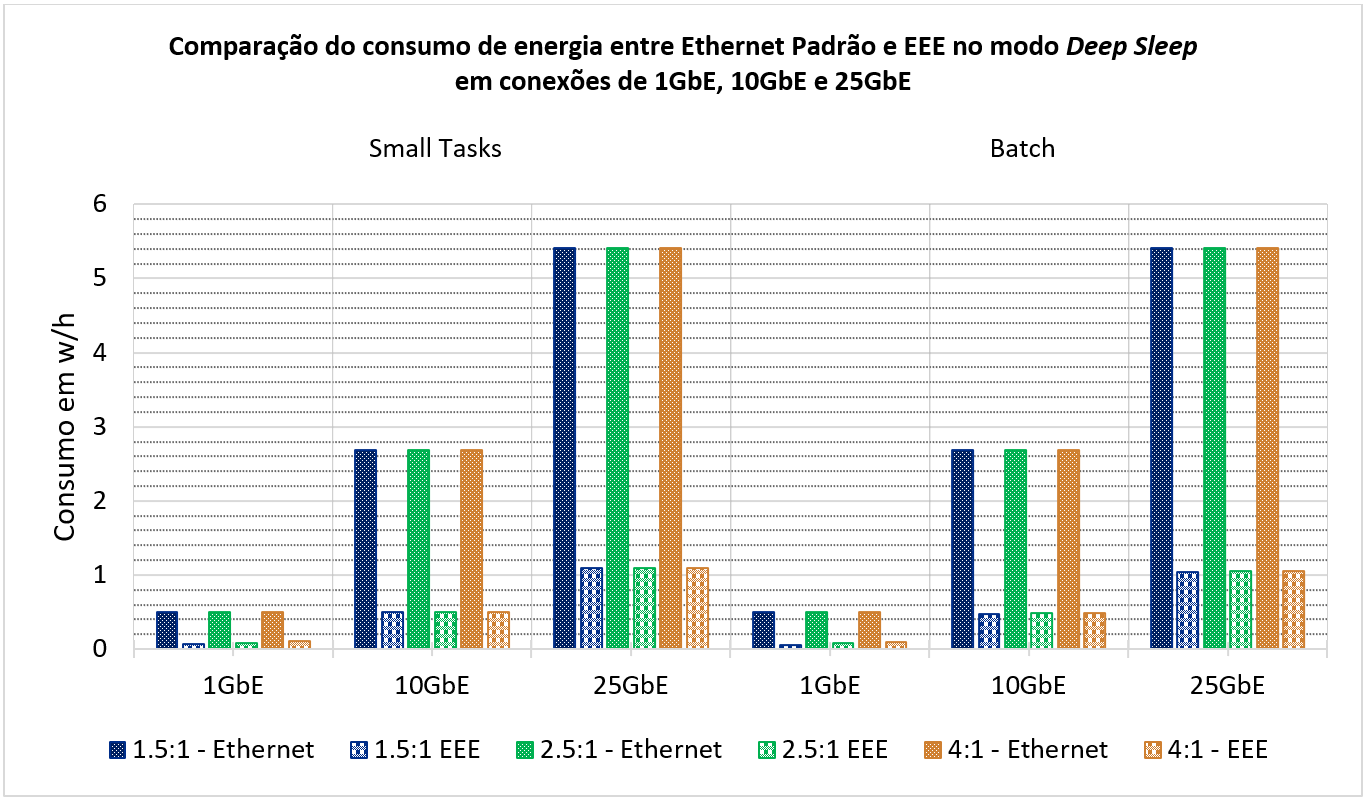
\includegraphics[width=16cm]{4-EEEHadoop/Image1_EEEConsumption1-10-25.PNG}
    \caption{\centering Comparação do consumo de energia entre \emph{Ethernet} Padrão e EEE no modo \emph{Deep Sleep} em conexões de 1GbE, 10GbE e 25GbE}
    \label{fig:EEEConsumption1-10-25}
\end{figure}

\begin{figure}[htp]
    \centering
    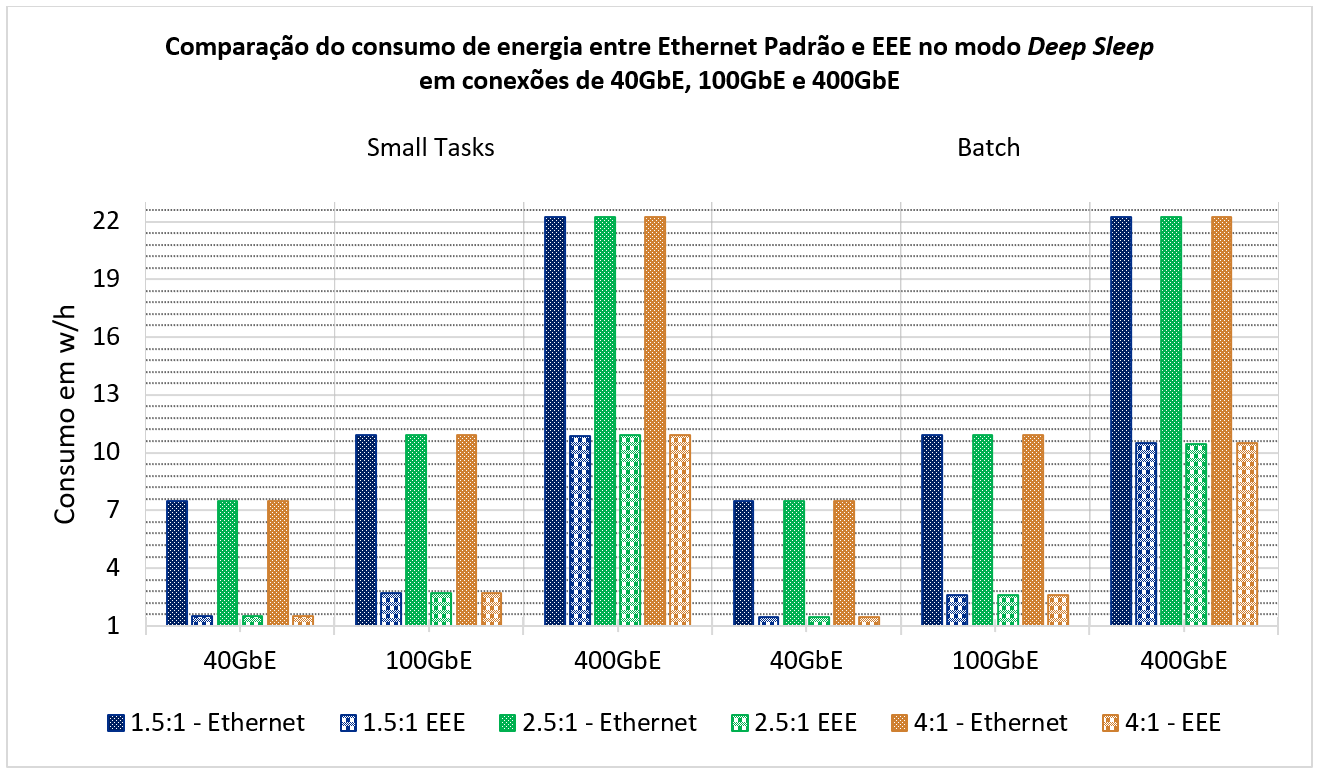
\includegraphics[width=16cm]{4-EEEHadoop/Image2_EEEConsumption40-100-400.PNG}
    \caption{\centering Comparação do consumo de energia entre \emph{Ethernet} Padrão e EEE no modo \emph{Deep Sleep} em conexões de 40GbE, 100GbE e 400GbE}
    \label{fig:EEEConsumption40-100-400}
\end{figure}

\begin{figure}[htp]
    \centering
    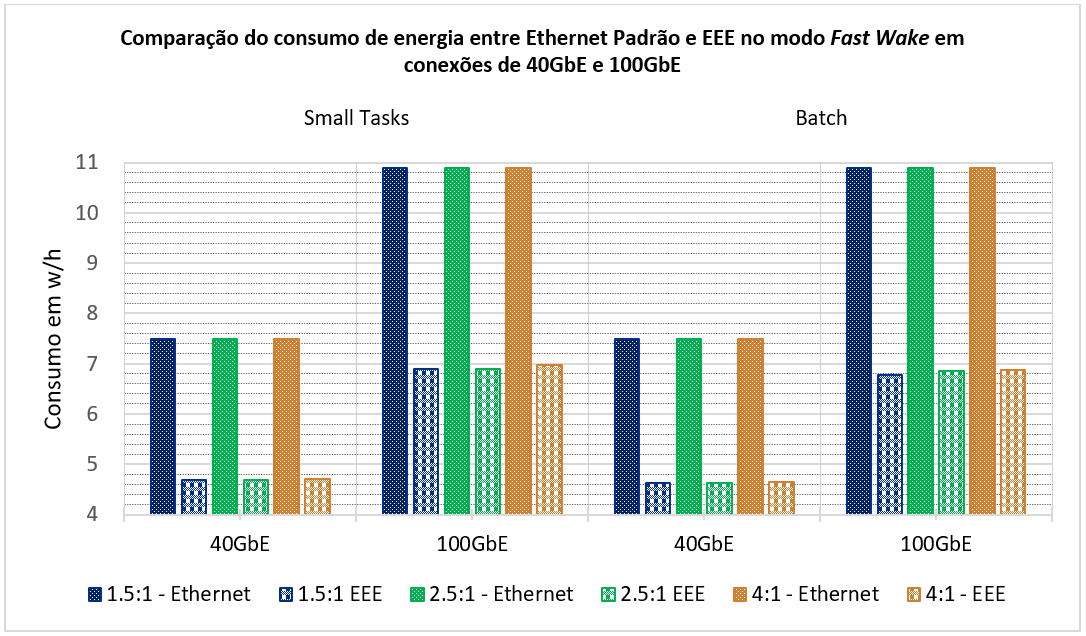
\includegraphics[width=16cm]{4-EEEHadoop/Image5_EEEConsumption40-100-FastWakeMode.PNG}
    \caption{\centering Comparação do consumo de energia entre \emph{Ethernet} Padrão e EEE no modo \emph{Fast Wake} em conexões de 40GbE e 100GbE}
    \label{fig:EEEConsumption100-400FastWakeMode}
\end{figure}

Através das simulações com o modo \textbf{\emph{Deep Sleep}} do EEE encontramos os dados mostrados nas figuras 4.1 e 4.2, que demonstram a economia de energia em \emph{Jobs MapReduce} em \emph{clusters}{} Hadoop 3.x, com reduções médias de 0,5w/h para 0,080w/h em links de 1GbE - redução de 83,89\%; 2,68w/h para 0,490w/h em 10GbE - redução de 81,68\%; de 5,41w/h para 1,072w/h em 25GbE - redução de 80,12\%; 7,49w/h para 1,487w/h em 40GbE - redução de 80,14\%; de 10,89w/h para 2,646w/h em 100GbE - redução de 75,69\%; e de 22,21w/h para 10,685w/h em 400GbE - redução de 51,89.

Usando a configuração de topologia de rede \emph{leaf-spine} recomendada pela Cisco, com uma taxa de assinatura excessiva igual a 4:1, encontramos resultados que, como em \cite{silva2018eon}; \cite{e2015exploring}; \cite{e2017energy}, apontam para economias de energia semelhantes habilitando o EEE no modo \textbf{\emph{Deep Sleep}} ao executar \emph{Small Tasks} e \emph{Batch Jobs}, no entanto, os \emph{Batch Jobs} tiveram um desempenho ligeiramente melhor.

Como pode-se observar na figura 4.3, ao habitarmos o EEE no modo \textbf{\emph{Fast Wake}} para as conexões de 40GbE e 100GbE, percebe-se uma economia de energia relativamente menor do que comparado ao modo \textbf{\emph{Deep Sleep}}, de 7,49w/h para 4,634w/h em conexões de 40GbE - redução de 38,13\%, e de 10,89w/h para 6,916w/h - redução de 36,49\% em conexões de 100GbE respectivamente. Em contrapartida, o desempenho foi melhor como detalhado na próxima seção.

\section{Desempenho}

Esta seção contém os dados de performance obtidos das simulações com topologia \emph{leaf-spine} e conexões de 1GbE e 10GbE; 1GbE e 25GbE; 10GbE e 100GbE; 10GbE e 400GbE; 25GbE e 400GbE; e, finalmente, 40GbE e 400GbE. O restante da metodologia empregada pode ser visualizada no Capítulo 3 de forma detalhada.

Ao contrário do que afirmam os fornecedores de equipamentos, nossos testes demonstram que é possível obter uma boa economia de energia habilitando o \emph{Energy Efficient Ethernet} no modo \textbf{\emph{Deep Sleep}}, com uma perda média de desempenho de praticamente zero para links de 1GbE - 0,21\%; 10GbE - 0,94\%; e 25GbE - 1,52\%; ou razoável no caso de 40GbE - 2,85\% conforme mostrado nas figuras 4.4 e 4.5. Para links de 100GbE e 400GbE há uma boa economia de energia, mas com uma perda de desempenho que não é considerada ideal, em torno de 4,55\% e 8,58\% respectivamente.

Em geral, ao habilitar o EEE em modo \textbf{\emph{Deep Sleep}} no \emph{cluster}, percebe-se que os \emph{Batch Jobs} obtêm melhor economia de energia e desempenho em relação aos \emph{Small Tasks}. Ainda é possível observar um cenário específico, em que ao diminuir a taxa de assinatura excessiva da rede para 1.5:1 em links 1GbE, os \emph{Batch Jobs} obtiveram uma melhora significativamente maior na economia de energia e no desempenho em comparação com outras conexões.

\begin{figure}[htp]
    \centering
    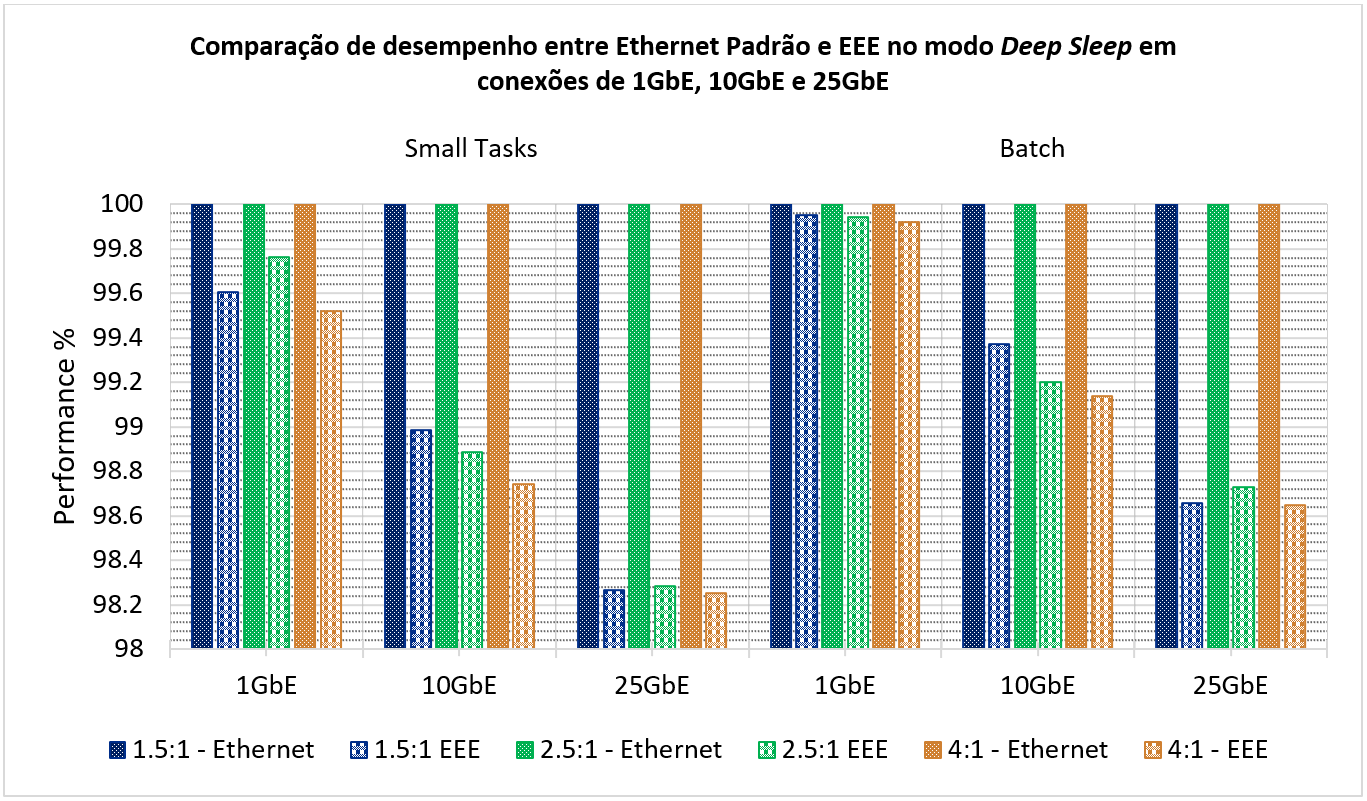
\includegraphics[width=16cm]{4-EEEHadoop/Image3_EEEPerformance1-10-25.PNG}
    \caption{\centering Comparação de desempenho entre \emph{Ethernet} Padrão e EEE no modo \emph{Deep Sleep} em conexões de 1GbE, 10GbE e 25GbE}
    \label{fig:EEEPerformance1-10-25}
\end{figure}

\begin{figure}[htp]
    \centering
    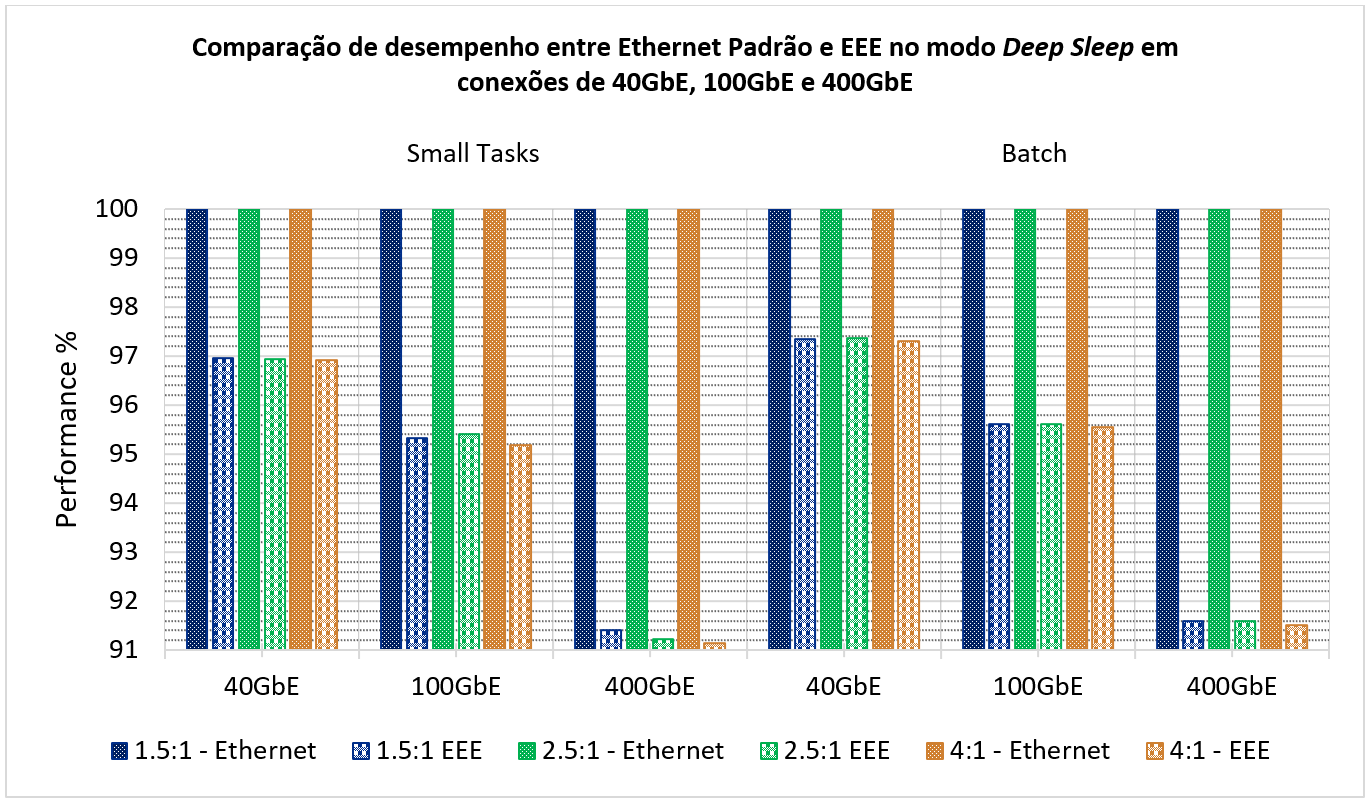
\includegraphics[width=16cm]{4-EEEHadoop/Image4_EEEPerformance40-100-400.PNG}
    \caption{\centering Comparação de desempenho entre \emph{Ethernet} Padrão e EEE no modo \emph{Deep Sleep} em conexões de 40GbE, 100GbE e 400GbE}
    \label{fig:EEEPerformance40-100-400}
\end{figure}

\begin{figure}[htp]
    \centering
    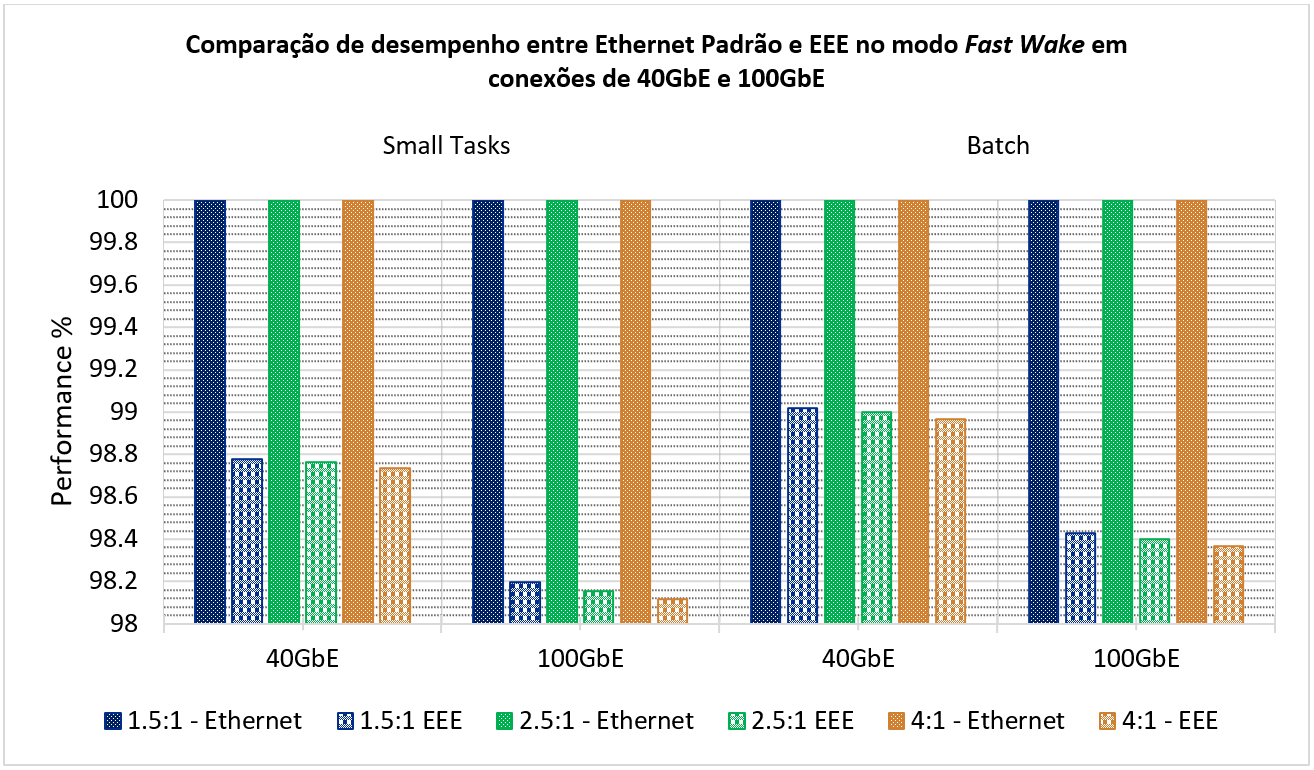
\includegraphics[width=16cm]{4-EEEHadoop/Image6_EEEPerformance40-100-FastWakeMode.PNG}
    \caption{\centering Comparação de desempenho entre \emph{Ethernet} Padrão e EEE no modo \emph{Fast Wake} em conexões de 40GbE e 100GbE}
    \label{fig:EEEPerformance40-100FastWake}
\end{figure}

Ao utilizarmos o modo \textbf{\emph{Fast Wake}} do EEE em nossas simulações, foi possível notar que embora este modo não forneça uma economia de energia como o modo \textbf{\emph{Deep Sleep}}, ele não afeta o desempenho de forma que seja considerável, com uma perda de 1,2\% no caso das conexões de 40GbE e 1,8\% em conexões de 100GbE, tornando-se assim uma opção interessante para as indústrias que buscam um balanceamento entre economia de energia e desempenho.  

As perdas de desempenho mais significativas encontradas para os links de 100GbE e 400GbE com o modo \textbf{\emph{Deep Sleep}} ocorreram porque em determinados momentos é necessário acordar um link para transmitir um único \emph{frame}, o que causa penalidades de latência e consumo de energia em termos relativos que são agravadas de acordo com a largura de banda \cite{jiang2021modeling}; \cite{reviriego2009performance}; \cite{reviriego2010burst}; \cite{e2017energy}. Se os momentos de \emph{wake} do EEE puderem ser controlados para evitar transmissões de um \emph{frame} único, pode ser possível obter economia de energia com perdas de desempenho baixas ou nulas para estas conexões.

\section{Considerações Finais}

Neste capítulo, apresentamos uma análise do impacto ao habilitar ao \emph{Energy Efficient Ethernet} nos modos \textbf{\emph{Deep Sleep}} e \textbf{\emph{Fast Wake}} em \emph{clusters MapReduce} que utilizam o \emph{framework} Apache Hadoop 3.x. Avaliamos execuções de \emph{Small Tasks} e \emph{Batch Jobs} com EEE em diversos \emph{clusters} simulados, e no modo \textbf{\emph{Deep Sleep}} encontramos economia de energia entre 78\% e 82\% para links de até 40GbE sem perda considerável de desempenho, entre 0,21\% e 2,85 \%. Para links de 100GbE e 400GbE houve uma economia de energia significativa de 75,69\% e 51,88\% respectivamente, mas com uma taxa de perda de desempenho considerável de 4,55\% e 8,58\%, o que não é particularmente interessante em \emph{Batch Jobs}. Quando optamos pelo uso do modo \textbf{\emph{Fast Wake}} do EEE, obtivemos uma redução do consumo de 7,49w/h para 4,634w/h em conexões de 40GbE, e de 10,89w/h para 6,916w/h em conexões de 100GbE, com uma perda de performance de 1.2\% e 1.8\%.

Em termos de custo-benefício para \emph{data centers}, o recomendado para conexões de até 40GbE é habilitar o EEE no modo \textbf{\emph{Deep Sleep}}, o que resulta em uma boa redução do consumo de energia e uma taxa de perda de desempenho baixa ou nula. Para conexões de 100GbE o recomendado é habilitar o modo \textbf{\emph{Fast Wake}} do EEE, obtendo assim um balanceamento entre consumo de energia e performance. Para conexões de 400GbE habilitar o EEE não é interessante, pois há uma perda de 8,58\% do desempenho.

O problema de latência e economia de energia encontrado em conexões acima de 100GbE com \textbf{\emph{Deep Sleep}} são causados por ter que acordar o link de tempos em tempos para transmitir um único \emph{frame}. Para resolver este problema, no próximo capítulo combinamos o \emph{Energy Efficient Ethernet} com \emph{Packet Coalescing}, \emph{Random Early Detection}, \emph{Controlled Delay}  e \emph{Explicit Congestion Notification}, podendo assim configurar de forma manual e inteligente quando os links devem ser acordados do modo LPI para transmissões de pacotes.

	% metodologia
\chapter{Energy Efficient Ethernet em Clusters Hadoop MapReduce}

Neste capítulo são apresentados os resultados das simulações de \emph{clusters Hadoop 3.x MapReduce} utilizando a ferramenta NetSLS e o \emph{Energy Efficient Ethernet} em modo \emph{Fast Wake} e \emph{Deep Sleep}. Através destes dados mostramos que uma boa economia de energia pode ser obtida em conexões de até 40GbE, enquanto conexões acima de 100GbE possuem problemas de performance quando o EEE está habilitado no modo \emph{Deep Sleep}.

\section{Economia de Energia}

Esta seção contém os dados de economia de energia obtidos das simulações com topologia \emph{leaf-spine} e conexões de 1GbE e 10GbE; 1GbE e 25GbE; 10GbE e 100GbE; 10GbE e 400GbE; 25GbE e 400GbE; e, finalmente, 40GbE e 400GbE. O restante da metodologia empregada pode ser visualizada no Capítulo 3 de forma detalhada.

\begin{figure}[htp]
    \centering
    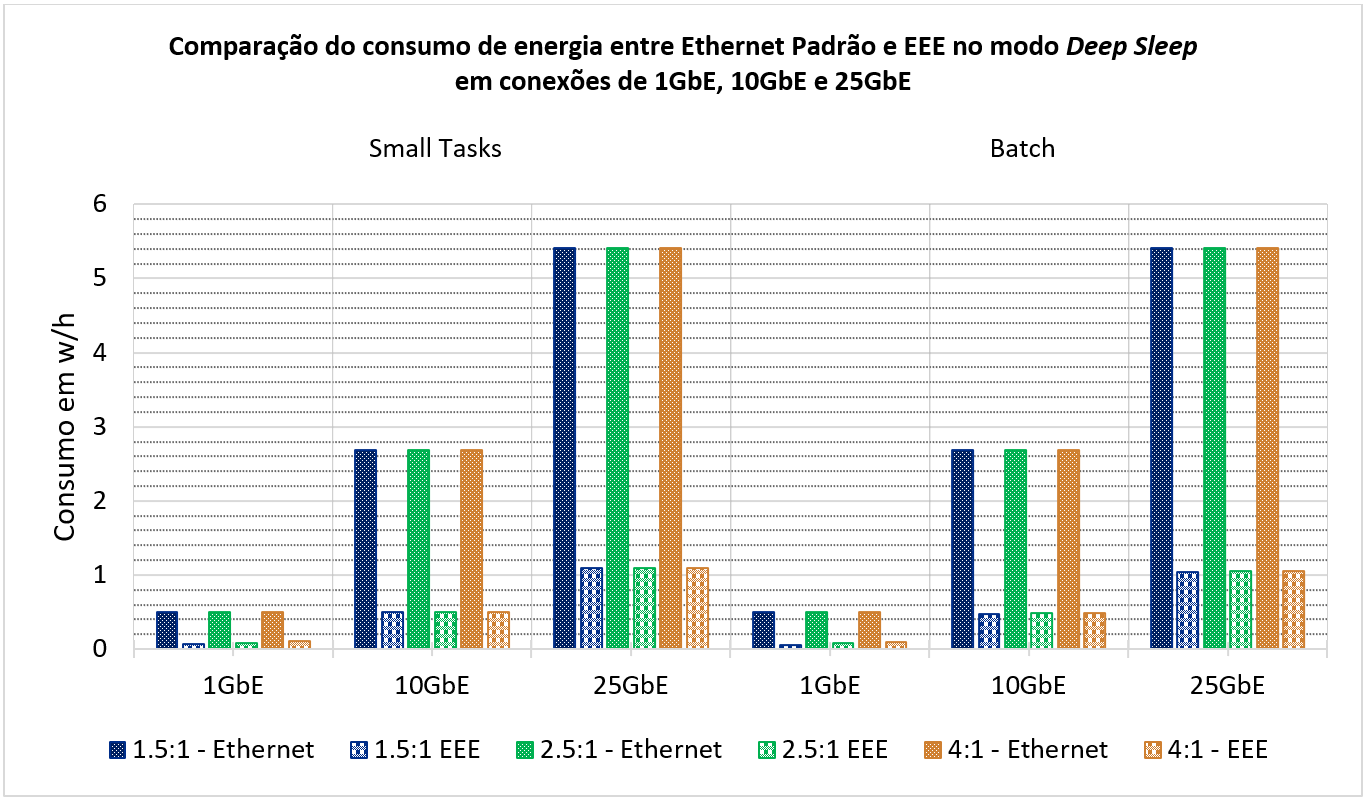
\includegraphics[width=16cm]{4-EEEHadoop/Image1_EEEConsumption1-10-25.PNG}
    \caption{\centering Comparação do consumo de energia entre \emph{Ethernet} Padrão e EEE no modo \emph{Deep Sleep} em conexões de 1GbE, 10GbE e 25GbE}
    \label{fig:EEEConsumption1-10-25}
\end{figure}

\begin{figure}[htp]
    \centering
    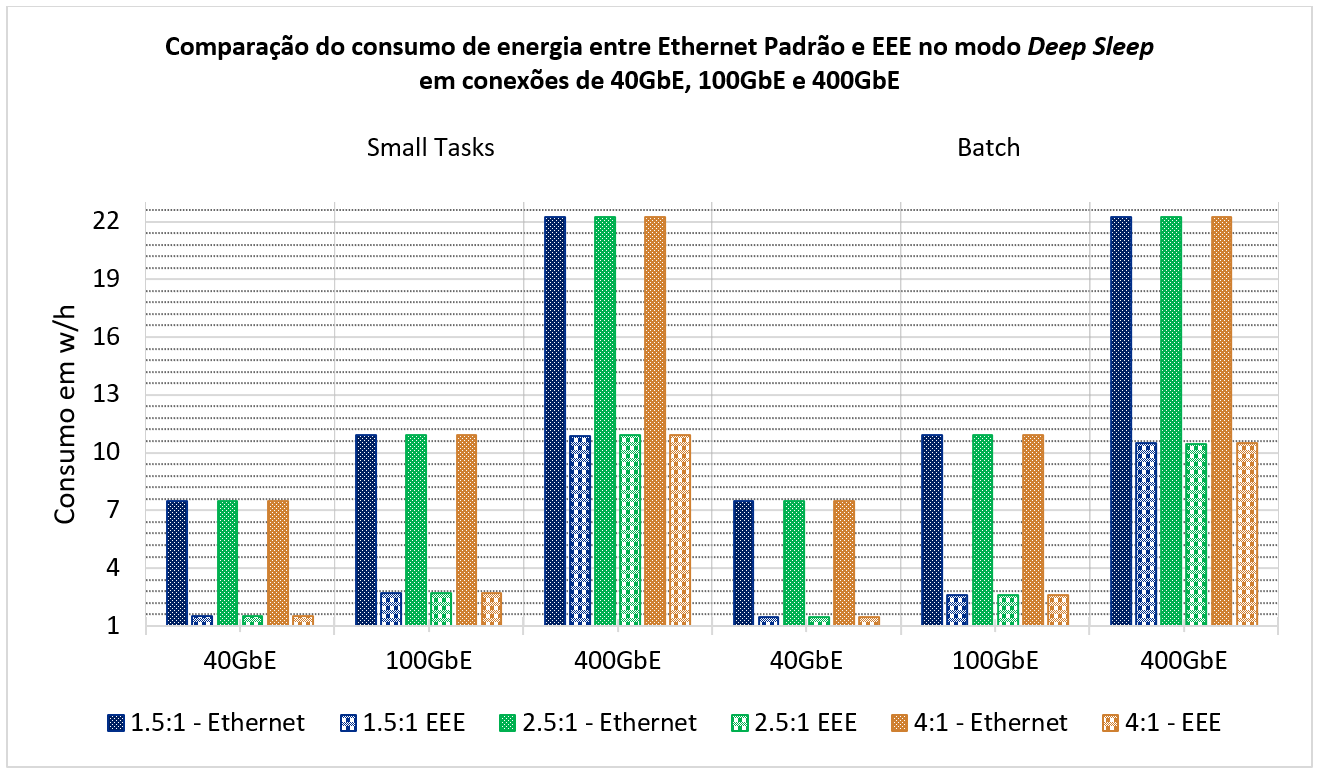
\includegraphics[width=16cm]{4-EEEHadoop/Image2_EEEConsumption40-100-400.PNG}
    \caption{\centering Comparação do consumo de energia entre \emph{Ethernet} Padrão e EEE no modo \emph{Deep Sleep} em conexões de 40GbE, 100GbE e 400GbE}
    \label{fig:EEEConsumption40-100-400}
\end{figure}

\begin{figure}[htp]
    \centering
    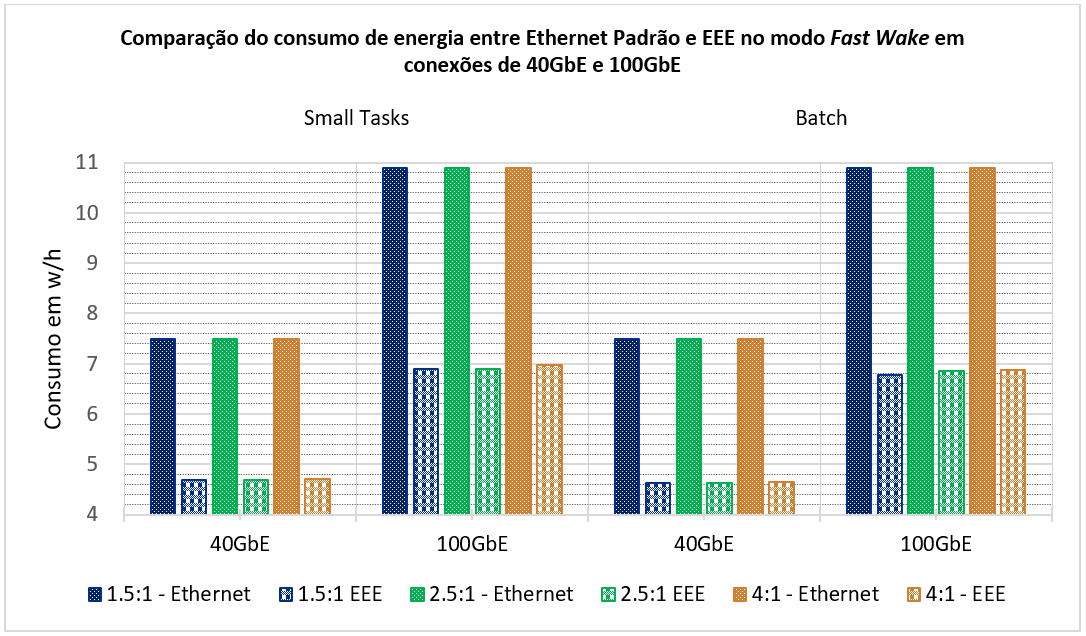
\includegraphics[width=16cm]{4-EEEHadoop/Image5_EEEConsumption40-100-FastWakeMode.PNG}
    \caption{\centering Comparação do consumo de energia entre \emph{Ethernet} Padrão e EEE no modo \emph{Fast Wake} em conexões de 40GbE e 100GbE}
    \label{fig:EEEConsumption100-400FastWakeMode}
\end{figure}

Através das simulações com o modo \textbf{\emph{Deep Sleep}} do EEE encontramos os dados mostrados nas figuras 4.1 e 4.2, que demonstram a economia de energia em \emph{Jobs MapReduce} em \emph{clusters}{} Hadoop 3.x, com reduções médias de 0,5w/h para 0,080w/h em links de 1GbE - redução de 83,89\%; 2,68w/h para 0,490w/h em 10GbE - redução de 81,68\%; de 5,41w/h para 1,072w/h em 25GbE - redução de 80,12\%; 7,49w/h para 1,487w/h em 40GbE - redução de 80,14\%; de 10,89w/h para 2,646w/h em 100GbE - redução de 75,69\%; e de 22,21w/h para 10,685w/h em 400GbE - redução de 51,89.

Usando a configuração de topologia de rede \emph{leaf-spine} recomendada pela Cisco, com uma taxa de assinatura excessiva igual a 4:1, encontramos resultados que, como em \cite{silva2018eon}; \cite{e2015exploring}; \cite{e2017energy}, apontam para economias de energia semelhantes habilitando o EEE no modo \textbf{\emph{Deep Sleep}} ao executar \emph{Small Tasks} e \emph{Batch Jobs}, no entanto, os \emph{Batch Jobs} tiveram um desempenho ligeiramente melhor.

Como pode-se observar na figura 4.3, ao habitarmos o EEE no modo \textbf{\emph{Fast Wake}} para as conexões de 40GbE e 100GbE, percebe-se uma economia de energia relativamente menor do que comparado ao modo \textbf{\emph{Deep Sleep}}, de 7,49w/h para 4,634w/h em conexões de 40GbE - redução de 38,13\%, e de 10,89w/h para 6,916w/h - redução de 36,49\% em conexões de 100GbE respectivamente. Em contrapartida, o desempenho foi melhor como detalhado na próxima seção.

\section{Desempenho}

Esta seção contém os dados de performance obtidos das simulações com topologia \emph{leaf-spine} e conexões de 1GbE e 10GbE; 1GbE e 25GbE; 10GbE e 100GbE; 10GbE e 400GbE; 25GbE e 400GbE; e, finalmente, 40GbE e 400GbE. O restante da metodologia empregada pode ser visualizada no Capítulo 3 de forma detalhada.

Ao contrário do que afirmam os fornecedores de equipamentos, nossos testes demonstram que é possível obter uma boa economia de energia habilitando o \emph{Energy Efficient Ethernet} no modo \textbf{\emph{Deep Sleep}}, com uma perda média de desempenho de praticamente zero para links de 1GbE - 0,21\%; 10GbE - 0,94\%; e 25GbE - 1,52\%; ou razoável no caso de 40GbE - 2,85\% conforme mostrado nas figuras 4.4 e 4.5. Para links de 100GbE e 400GbE há uma boa economia de energia, mas com uma perda de desempenho que não é considerada ideal, em torno de 4,55\% e 8,58\% respectivamente.

Em geral, ao habilitar o EEE em modo \textbf{\emph{Deep Sleep}} no \emph{cluster}, percebe-se que os \emph{Batch Jobs} obtêm melhor economia de energia e desempenho em relação aos \emph{Small Tasks}. Ainda é possível observar um cenário específico, em que ao diminuir a taxa de assinatura excessiva da rede para 1.5:1 em links 1GbE, os \emph{Batch Jobs} obtiveram uma melhora significativamente maior na economia de energia e no desempenho em comparação com outras conexões.

\begin{figure}[htp]
    \centering
    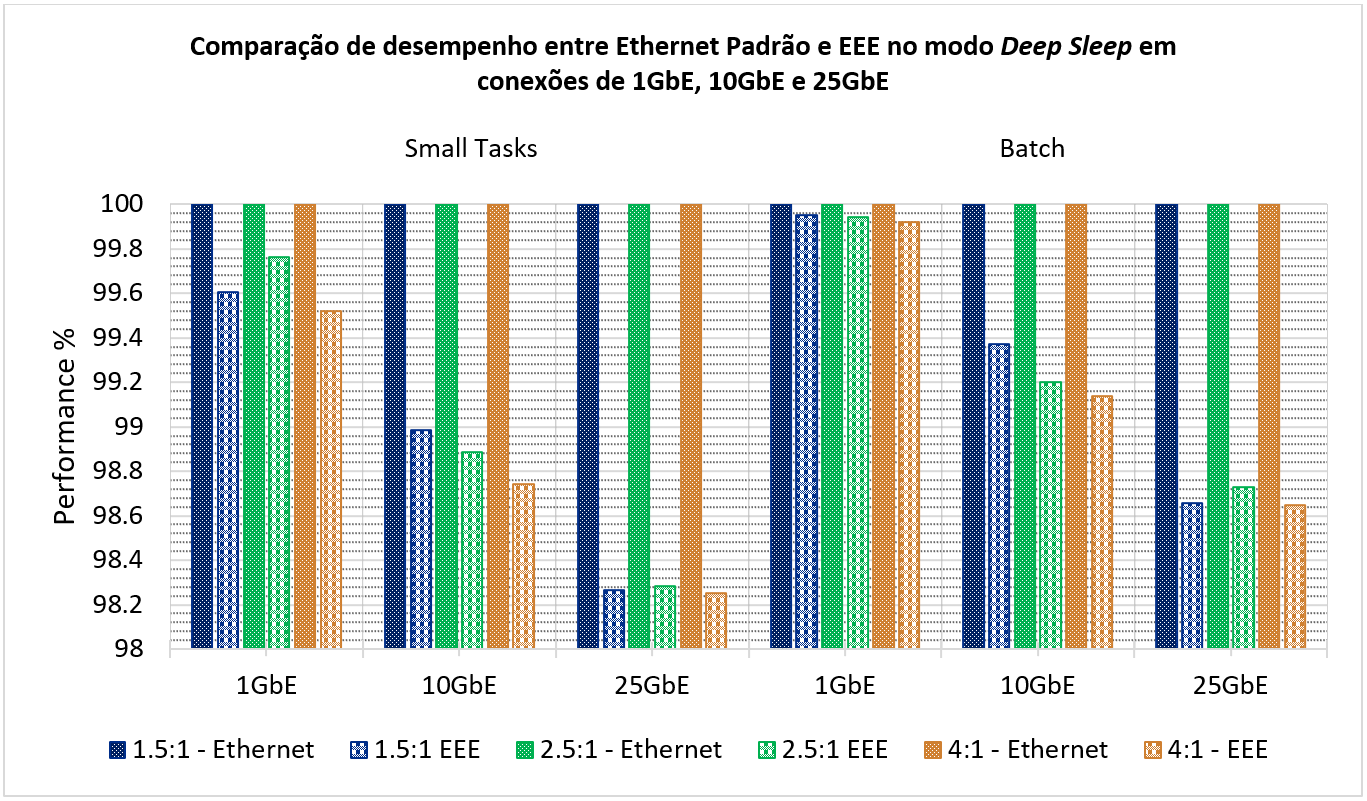
\includegraphics[width=16cm]{4-EEEHadoop/Image3_EEEPerformance1-10-25.PNG}
    \caption{\centering Comparação de desempenho entre \emph{Ethernet} Padrão e EEE no modo \emph{Deep Sleep} em conexões de 1GbE, 10GbE e 25GbE}
    \label{fig:EEEPerformance1-10-25}
\end{figure}

\begin{figure}[htp]
    \centering
    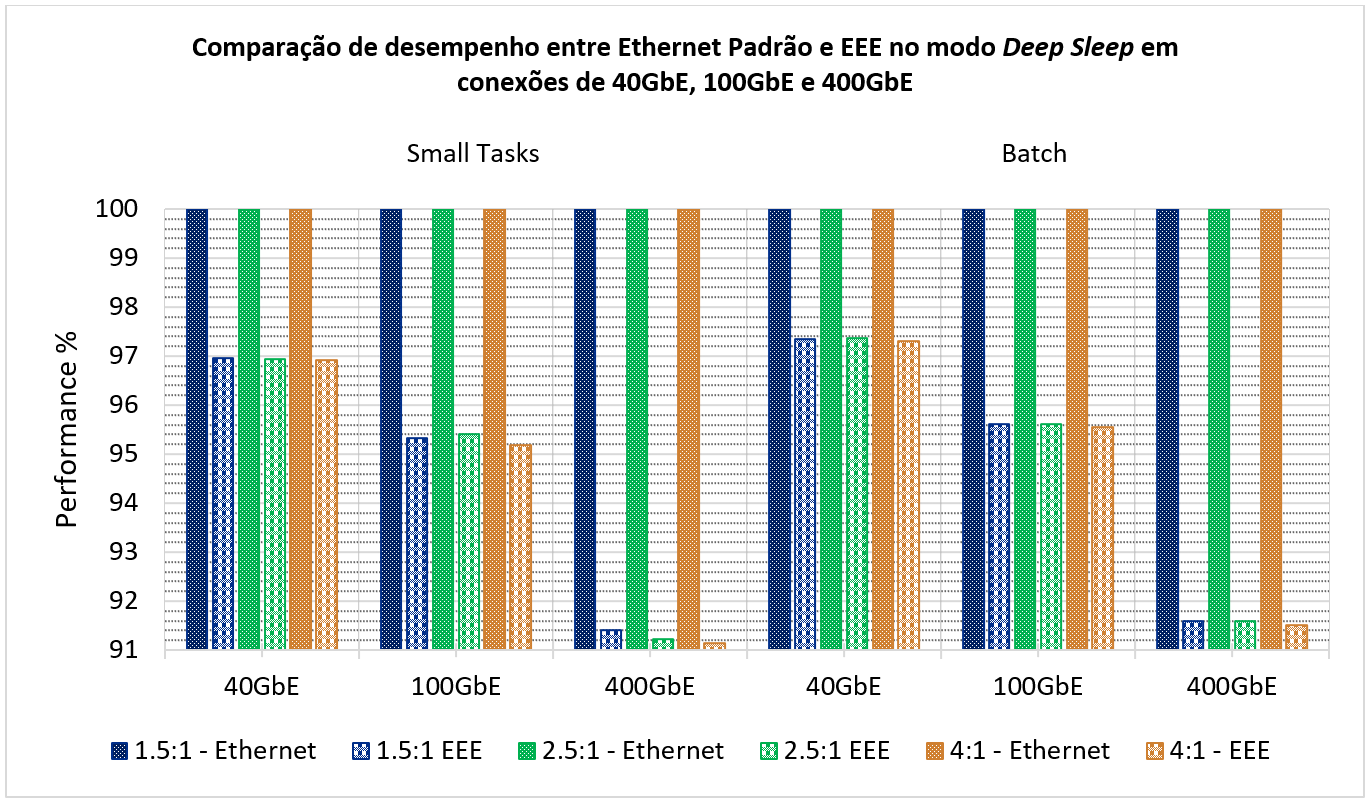
\includegraphics[width=16cm]{4-EEEHadoop/Image4_EEEPerformance40-100-400.PNG}
    \caption{\centering Comparação de desempenho entre \emph{Ethernet} Padrão e EEE no modo \emph{Deep Sleep} em conexões de 40GbE, 100GbE e 400GbE}
    \label{fig:EEEPerformance40-100-400}
\end{figure}

\begin{figure}[htp]
    \centering
    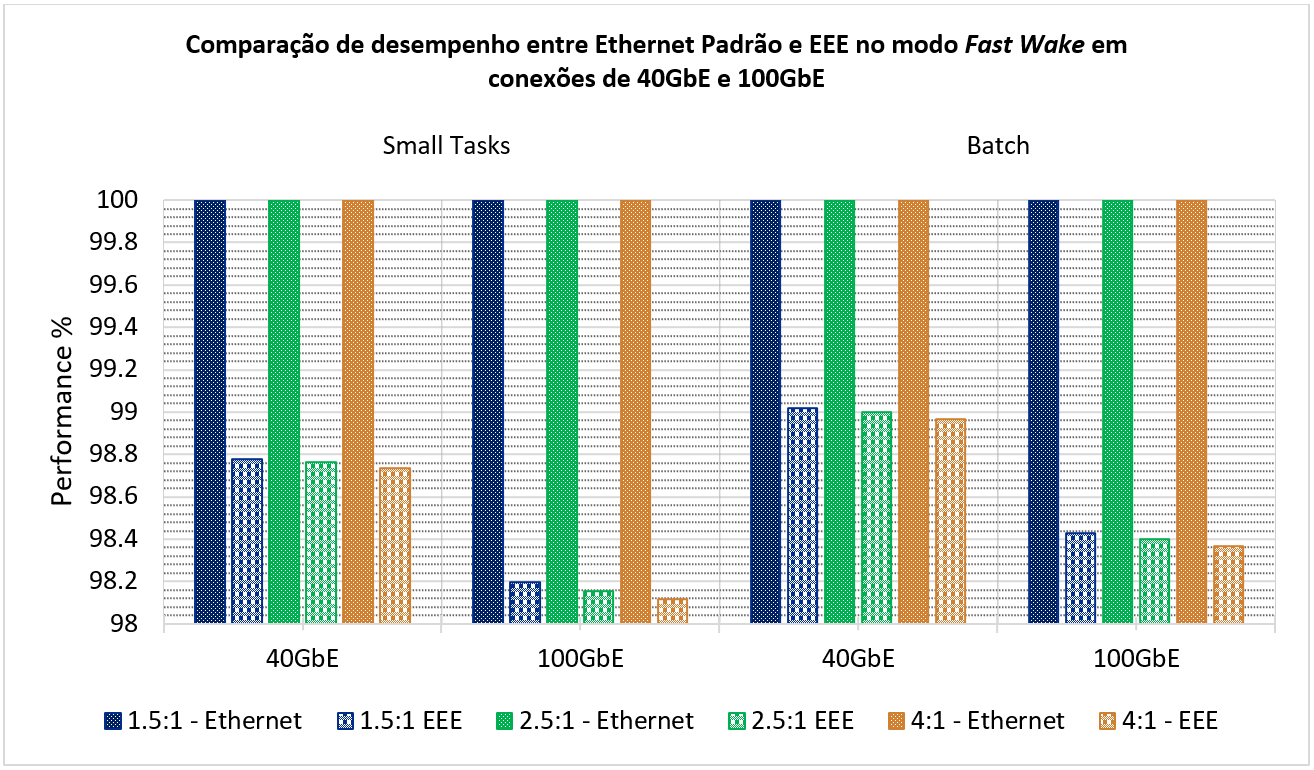
\includegraphics[width=16cm]{4-EEEHadoop/Image6_EEEPerformance40-100-FastWakeMode.PNG}
    \caption{\centering Comparação de desempenho entre \emph{Ethernet} Padrão e EEE no modo \emph{Fast Wake} em conexões de 40GbE e 100GbE}
    \label{fig:EEEPerformance40-100FastWake}
\end{figure}

Ao utilizarmos o modo \textbf{\emph{Fast Wake}} do EEE em nossas simulações, foi possível notar que embora este modo não forneça uma economia de energia como o modo \textbf{\emph{Deep Sleep}}, ele não afeta o desempenho de forma que seja considerável, com uma perda de 1,2\% no caso das conexões de 40GbE e 1,8\% em conexões de 100GbE, tornando-se assim uma opção interessante para as indústrias que buscam um balanceamento entre economia de energia e desempenho.  

As perdas de desempenho mais significativas encontradas para os links de 100GbE e 400GbE com o modo \textbf{\emph{Deep Sleep}} ocorreram porque em determinados momentos é necessário acordar um link para transmitir um único \emph{frame}, o que causa penalidades de latência e consumo de energia em termos relativos que são agravadas de acordo com a largura de banda \cite{jiang2021modeling}; \cite{reviriego2009performance}; \cite{reviriego2010burst}; \cite{e2017energy}. Se os momentos de \emph{wake} do EEE puderem ser controlados para evitar transmissões de um \emph{frame} único, pode ser possível obter economia de energia com perdas de desempenho baixas ou nulas para estas conexões.

\section{Considerações Finais}

Neste capítulo, apresentamos uma análise do impacto ao habilitar ao \emph{Energy Efficient Ethernet} nos modos \textbf{\emph{Deep Sleep}} e \textbf{\emph{Fast Wake}} em \emph{clusters MapReduce} que utilizam o \emph{framework} Apache Hadoop 3.x. Avaliamos execuções de \emph{Small Tasks} e \emph{Batch Jobs} com EEE em diversos \emph{clusters} simulados, e no modo \textbf{\emph{Deep Sleep}} encontramos economia de energia entre 78\% e 82\% para links de até 40GbE sem perda considerável de desempenho, entre 0,21\% e 2,85 \%. Para links de 100GbE e 400GbE houve uma economia de energia significativa de 75,69\% e 51,88\% respectivamente, mas com uma taxa de perda de desempenho considerável de 4,55\% e 8,58\%, o que não é particularmente interessante em \emph{Batch Jobs}. Quando optamos pelo uso do modo \textbf{\emph{Fast Wake}} do EEE, obtivemos uma redução do consumo de 7,49w/h para 4,634w/h em conexões de 40GbE, e de 10,89w/h para 6,916w/h em conexões de 100GbE, com uma perda de performance de 1.2\% e 1.8\%.

Em termos de custo-benefício para \emph{data centers}, o recomendado para conexões de até 40GbE é habilitar o EEE no modo \textbf{\emph{Deep Sleep}}, o que resulta em uma boa redução do consumo de energia e uma taxa de perda de desempenho baixa ou nula. Para conexões de 100GbE o recomendado é habilitar o modo \textbf{\emph{Fast Wake}} do EEE, obtendo assim um balanceamento entre consumo de energia e performance. Para conexões de 400GbE habilitar o EEE não é interessante, pois há uma perda de 8,58\% do desempenho.

O problema de latência e economia de energia encontrado em conexões acima de 100GbE com \textbf{\emph{Deep Sleep}} são causados por ter que acordar o link de tempos em tempos para transmitir um único \emph{frame}. Para resolver este problema, no próximo capítulo combinamos o \emph{Energy Efficient Ethernet} com \emph{Packet Coalescing}, \emph{Random Early Detection}, \emph{Controlled Delay}  e \emph{Explicit Congestion Notification}, podendo assim configurar de forma manual e inteligente quando os links devem ser acordados do modo LPI para transmissões de pacotes.

		% resultados preliminares
\chapter{Energy Efficient Ethernet em Clusters Hadoop MapReduce}

Neste capítulo são apresentados os resultados das simulações de \emph{clusters Hadoop 3.x MapReduce} utilizando a ferramenta NetSLS e o \emph{Energy Efficient Ethernet} em modo \emph{Fast Wake} e \emph{Deep Sleep}. Através destes dados mostramos que uma boa economia de energia pode ser obtida em conexões de até 40GbE, enquanto conexões acima de 100GbE possuem problemas de performance quando o EEE está habilitado no modo \emph{Deep Sleep}.

\section{Economia de Energia}

Esta seção contém os dados de economia de energia obtidos das simulações com topologia \emph{leaf-spine} e conexões de 1GbE e 10GbE; 1GbE e 25GbE; 10GbE e 100GbE; 10GbE e 400GbE; 25GbE e 400GbE; e, finalmente, 40GbE e 400GbE. O restante da metodologia empregada pode ser visualizada no Capítulo 3 de forma detalhada.

\begin{figure}[htp]
    \centering
    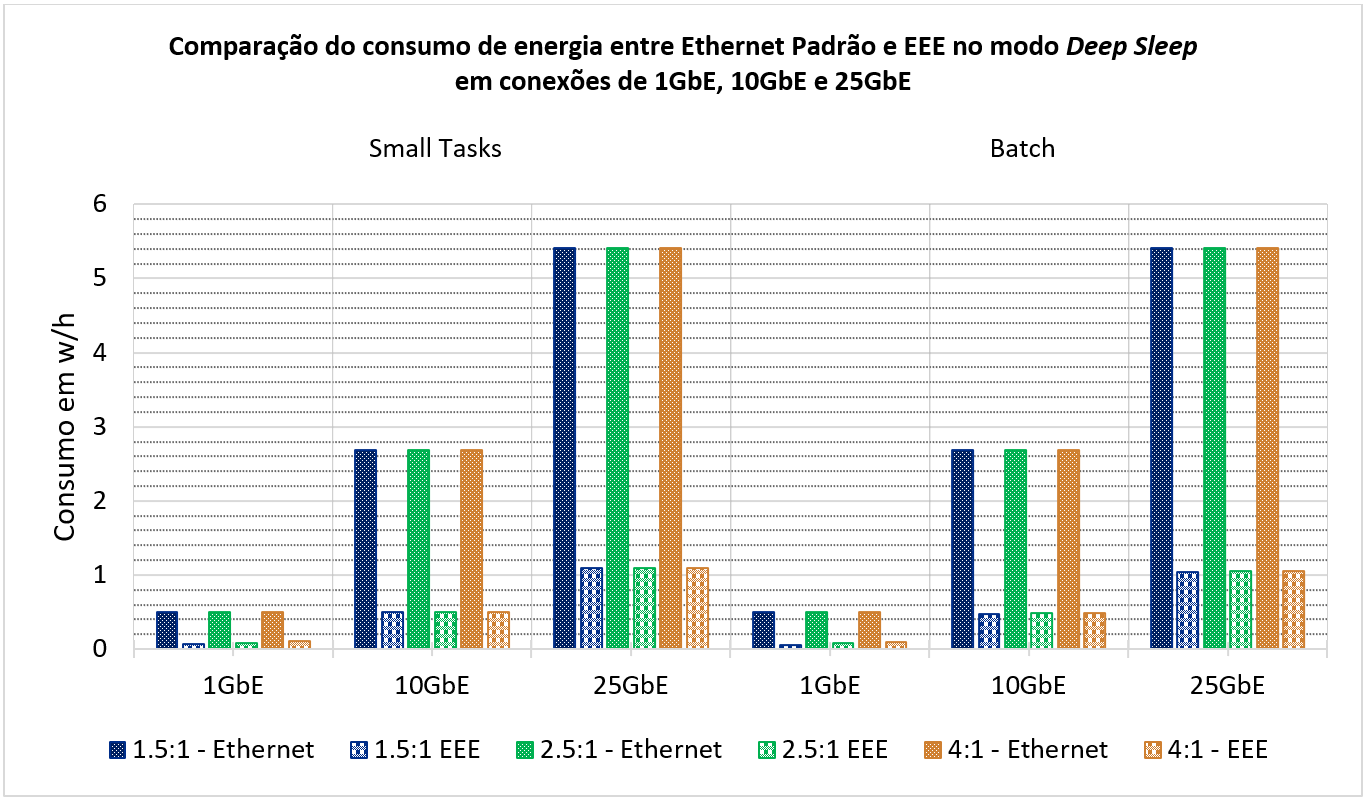
\includegraphics[width=16cm]{4-EEEHadoop/Image1_EEEConsumption1-10-25.PNG}
    \caption{\centering Comparação do consumo de energia entre \emph{Ethernet} Padrão e EEE no modo \emph{Deep Sleep} em conexões de 1GbE, 10GbE e 25GbE}
    \label{fig:EEEConsumption1-10-25}
\end{figure}

\begin{figure}[htp]
    \centering
    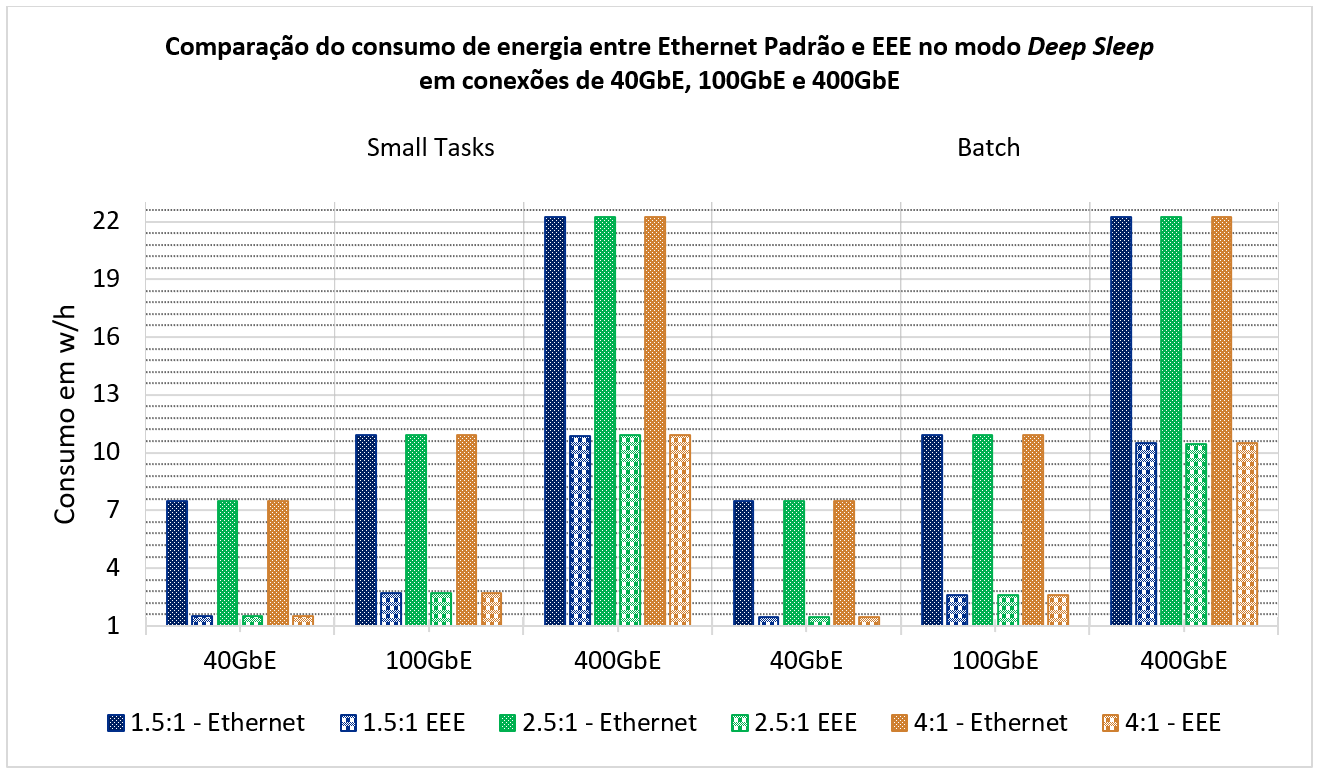
\includegraphics[width=16cm]{4-EEEHadoop/Image2_EEEConsumption40-100-400.PNG}
    \caption{\centering Comparação do consumo de energia entre \emph{Ethernet} Padrão e EEE no modo \emph{Deep Sleep} em conexões de 40GbE, 100GbE e 400GbE}
    \label{fig:EEEConsumption40-100-400}
\end{figure}

\begin{figure}[htp]
    \centering
    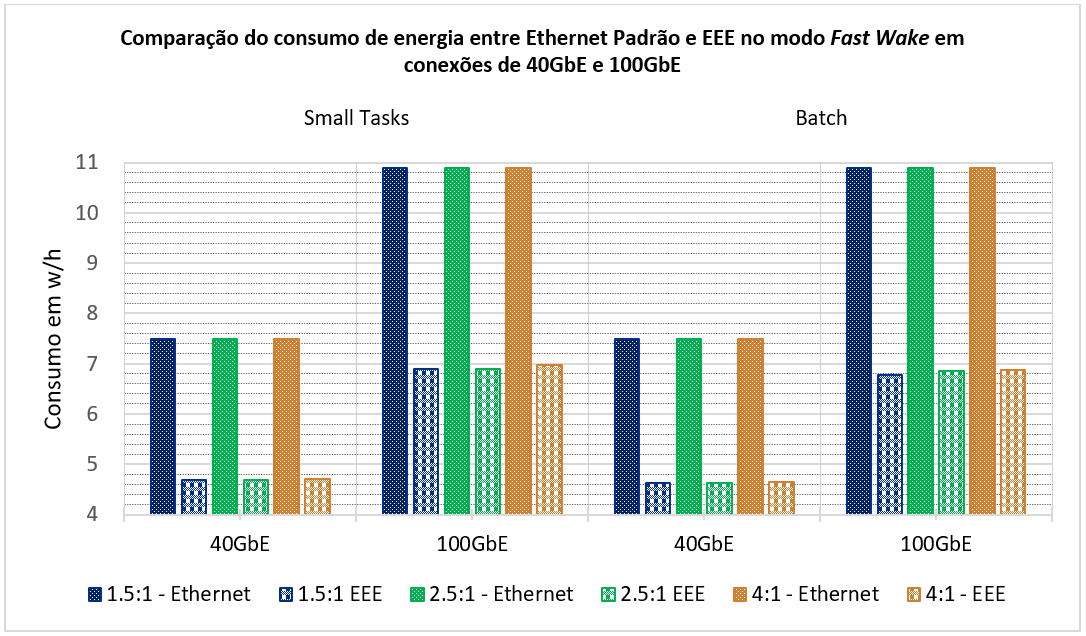
\includegraphics[width=16cm]{4-EEEHadoop/Image5_EEEConsumption40-100-FastWakeMode.PNG}
    \caption{\centering Comparação do consumo de energia entre \emph{Ethernet} Padrão e EEE no modo \emph{Fast Wake} em conexões de 40GbE e 100GbE}
    \label{fig:EEEConsumption100-400FastWakeMode}
\end{figure}

Através das simulações com o modo \textbf{\emph{Deep Sleep}} do EEE encontramos os dados mostrados nas figuras 4.1 e 4.2, que demonstram a economia de energia em \emph{Jobs MapReduce} em \emph{clusters}{} Hadoop 3.x, com reduções médias de 0,5w/h para 0,080w/h em links de 1GbE - redução de 83,89\%; 2,68w/h para 0,490w/h em 10GbE - redução de 81,68\%; de 5,41w/h para 1,072w/h em 25GbE - redução de 80,12\%; 7,49w/h para 1,487w/h em 40GbE - redução de 80,14\%; de 10,89w/h para 2,646w/h em 100GbE - redução de 75,69\%; e de 22,21w/h para 10,685w/h em 400GbE - redução de 51,89.

Usando a configuração de topologia de rede \emph{leaf-spine} recomendada pela Cisco, com uma taxa de assinatura excessiva igual a 4:1, encontramos resultados que, como em \cite{silva2018eon}; \cite{e2015exploring}; \cite{e2017energy}, apontam para economias de energia semelhantes habilitando o EEE no modo \textbf{\emph{Deep Sleep}} ao executar \emph{Small Tasks} e \emph{Batch Jobs}, no entanto, os \emph{Batch Jobs} tiveram um desempenho ligeiramente melhor.

Como pode-se observar na figura 4.3, ao habitarmos o EEE no modo \textbf{\emph{Fast Wake}} para as conexões de 40GbE e 100GbE, percebe-se uma economia de energia relativamente menor do que comparado ao modo \textbf{\emph{Deep Sleep}}, de 7,49w/h para 4,634w/h em conexões de 40GbE - redução de 38,13\%, e de 10,89w/h para 6,916w/h - redução de 36,49\% em conexões de 100GbE respectivamente. Em contrapartida, o desempenho foi melhor como detalhado na próxima seção.

\section{Desempenho}

Esta seção contém os dados de performance obtidos das simulações com topologia \emph{leaf-spine} e conexões de 1GbE e 10GbE; 1GbE e 25GbE; 10GbE e 100GbE; 10GbE e 400GbE; 25GbE e 400GbE; e, finalmente, 40GbE e 400GbE. O restante da metodologia empregada pode ser visualizada no Capítulo 3 de forma detalhada.

Ao contrário do que afirmam os fornecedores de equipamentos, nossos testes demonstram que é possível obter uma boa economia de energia habilitando o \emph{Energy Efficient Ethernet} no modo \textbf{\emph{Deep Sleep}}, com uma perda média de desempenho de praticamente zero para links de 1GbE - 0,21\%; 10GbE - 0,94\%; e 25GbE - 1,52\%; ou razoável no caso de 40GbE - 2,85\% conforme mostrado nas figuras 4.4 e 4.5. Para links de 100GbE e 400GbE há uma boa economia de energia, mas com uma perda de desempenho que não é considerada ideal, em torno de 4,55\% e 8,58\% respectivamente.

Em geral, ao habilitar o EEE em modo \textbf{\emph{Deep Sleep}} no \emph{cluster}, percebe-se que os \emph{Batch Jobs} obtêm melhor economia de energia e desempenho em relação aos \emph{Small Tasks}. Ainda é possível observar um cenário específico, em que ao diminuir a taxa de assinatura excessiva da rede para 1.5:1 em links 1GbE, os \emph{Batch Jobs} obtiveram uma melhora significativamente maior na economia de energia e no desempenho em comparação com outras conexões.

\begin{figure}[htp]
    \centering
    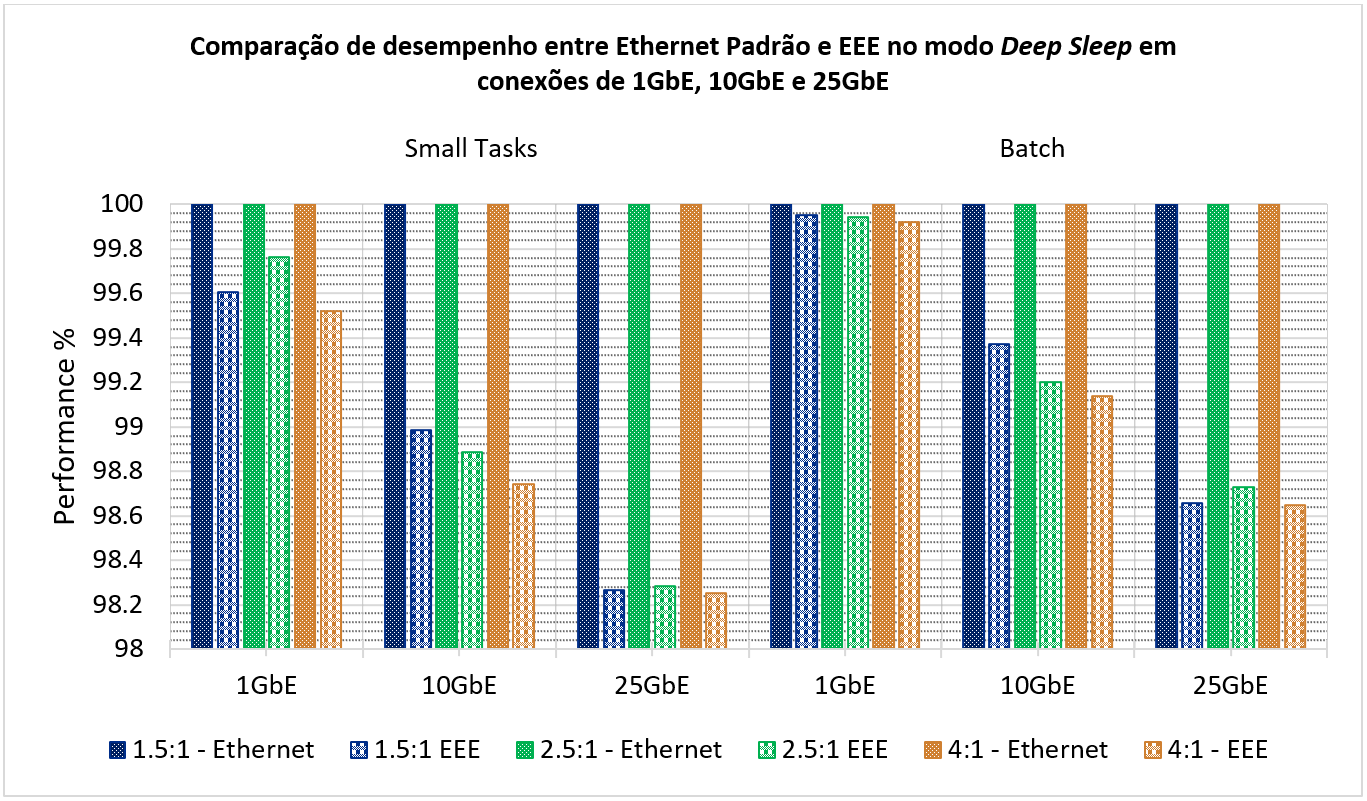
\includegraphics[width=16cm]{4-EEEHadoop/Image3_EEEPerformance1-10-25.PNG}
    \caption{\centering Comparação de desempenho entre \emph{Ethernet} Padrão e EEE no modo \emph{Deep Sleep} em conexões de 1GbE, 10GbE e 25GbE}
    \label{fig:EEEPerformance1-10-25}
\end{figure}

\begin{figure}[htp]
    \centering
    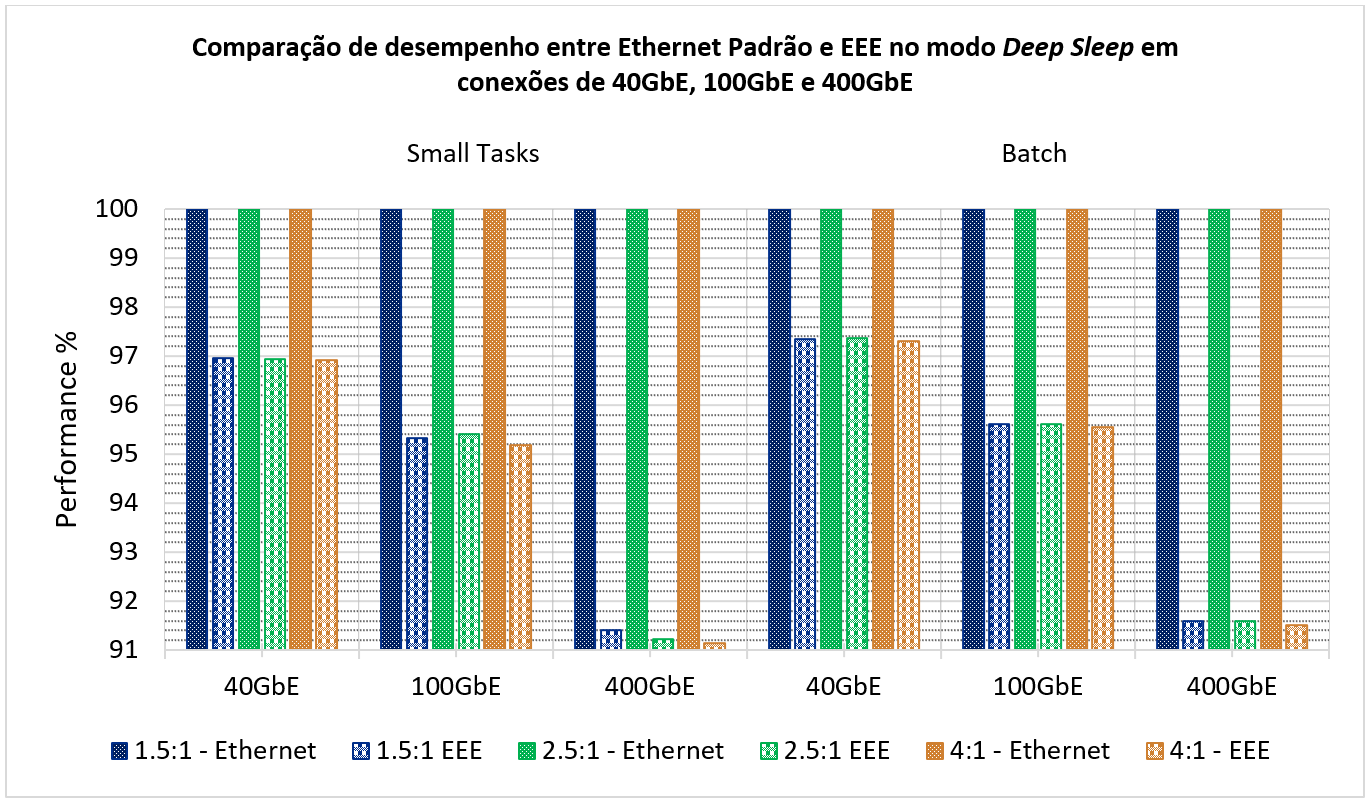
\includegraphics[width=16cm]{4-EEEHadoop/Image4_EEEPerformance40-100-400.PNG}
    \caption{\centering Comparação de desempenho entre \emph{Ethernet} Padrão e EEE no modo \emph{Deep Sleep} em conexões de 40GbE, 100GbE e 400GbE}
    \label{fig:EEEPerformance40-100-400}
\end{figure}

\begin{figure}[htp]
    \centering
    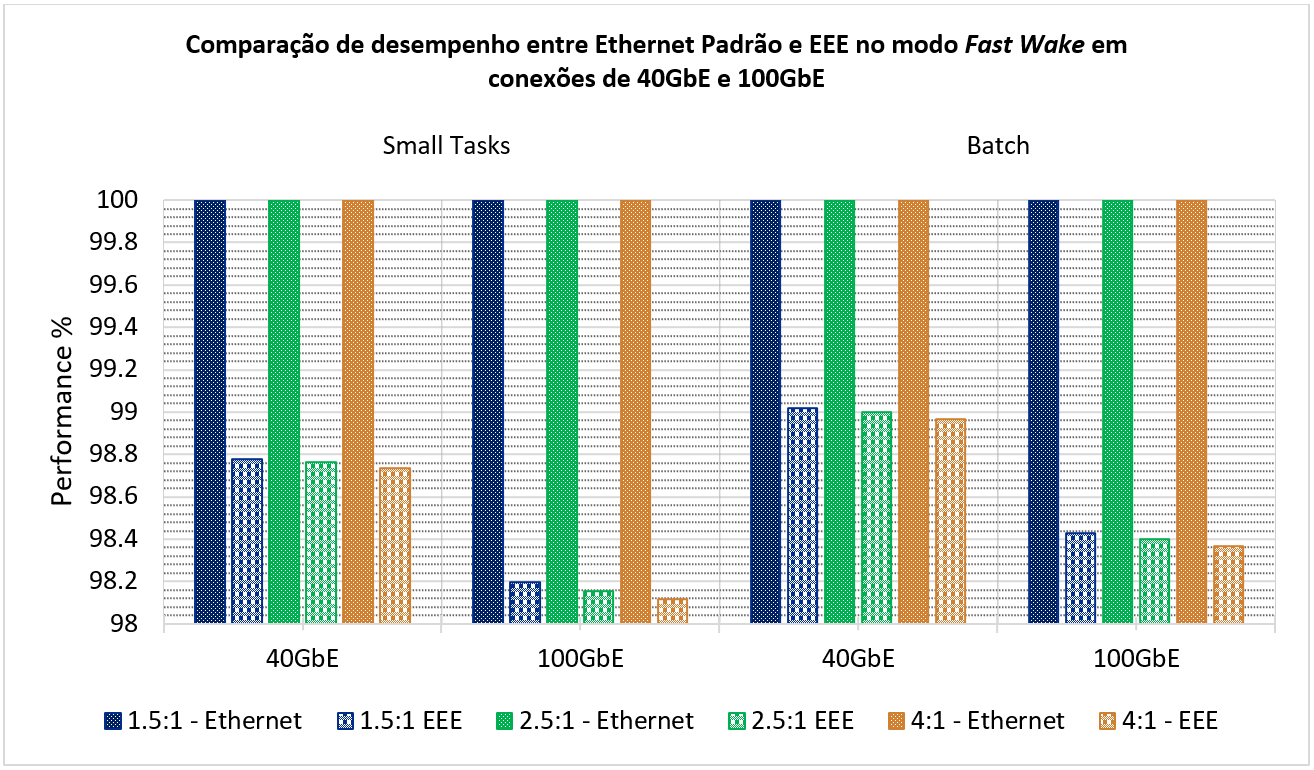
\includegraphics[width=16cm]{4-EEEHadoop/Image6_EEEPerformance40-100-FastWakeMode.PNG}
    \caption{\centering Comparação de desempenho entre \emph{Ethernet} Padrão e EEE no modo \emph{Fast Wake} em conexões de 40GbE e 100GbE}
    \label{fig:EEEPerformance40-100FastWake}
\end{figure}

Ao utilizarmos o modo \textbf{\emph{Fast Wake}} do EEE em nossas simulações, foi possível notar que embora este modo não forneça uma economia de energia como o modo \textbf{\emph{Deep Sleep}}, ele não afeta o desempenho de forma que seja considerável, com uma perda de 1,2\% no caso das conexões de 40GbE e 1,8\% em conexões de 100GbE, tornando-se assim uma opção interessante para as indústrias que buscam um balanceamento entre economia de energia e desempenho.  

As perdas de desempenho mais significativas encontradas para os links de 100GbE e 400GbE com o modo \textbf{\emph{Deep Sleep}} ocorreram porque em determinados momentos é necessário acordar um link para transmitir um único \emph{frame}, o que causa penalidades de latência e consumo de energia em termos relativos que são agravadas de acordo com a largura de banda \cite{jiang2021modeling}; \cite{reviriego2009performance}; \cite{reviriego2010burst}; \cite{e2017energy}. Se os momentos de \emph{wake} do EEE puderem ser controlados para evitar transmissões de um \emph{frame} único, pode ser possível obter economia de energia com perdas de desempenho baixas ou nulas para estas conexões.

\section{Considerações Finais}

Neste capítulo, apresentamos uma análise do impacto ao habilitar ao \emph{Energy Efficient Ethernet} nos modos \textbf{\emph{Deep Sleep}} e \textbf{\emph{Fast Wake}} em \emph{clusters MapReduce} que utilizam o \emph{framework} Apache Hadoop 3.x. Avaliamos execuções de \emph{Small Tasks} e \emph{Batch Jobs} com EEE em diversos \emph{clusters} simulados, e no modo \textbf{\emph{Deep Sleep}} encontramos economia de energia entre 78\% e 82\% para links de até 40GbE sem perda considerável de desempenho, entre 0,21\% e 2,85 \%. Para links de 100GbE e 400GbE houve uma economia de energia significativa de 75,69\% e 51,88\% respectivamente, mas com uma taxa de perda de desempenho considerável de 4,55\% e 8,58\%, o que não é particularmente interessante em \emph{Batch Jobs}. Quando optamos pelo uso do modo \textbf{\emph{Fast Wake}} do EEE, obtivemos uma redução do consumo de 7,49w/h para 4,634w/h em conexões de 40GbE, e de 10,89w/h para 6,916w/h em conexões de 100GbE, com uma perda de performance de 1.2\% e 1.8\%.

Em termos de custo-benefício para \emph{data centers}, o recomendado para conexões de até 40GbE é habilitar o EEE no modo \textbf{\emph{Deep Sleep}}, o que resulta em uma boa redução do consumo de energia e uma taxa de perda de desempenho baixa ou nula. Para conexões de 100GbE o recomendado é habilitar o modo \textbf{\emph{Fast Wake}} do EEE, obtendo assim um balanceamento entre consumo de energia e performance. Para conexões de 400GbE habilitar o EEE não é interessante, pois há uma perda de 8,58\% do desempenho.

O problema de latência e economia de energia encontrado em conexões acima de 100GbE com \textbf{\emph{Deep Sleep}} são causados por ter que acordar o link de tempos em tempos para transmitir um único \emph{frame}. Para resolver este problema, no próximo capítulo combinamos o \emph{Energy Efficient Ethernet} com \emph{Packet Coalescing}, \emph{Random Early Detection}, \emph{Controlled Delay}  e \emph{Explicit Congestion Notification}, podendo assim configurar de forma manual e inteligente quando os links devem ser acordados do modo LPI para transmissões de pacotes.

		% experimentação e validação
\chapter{Energy Efficient Ethernet em Clusters Hadoop MapReduce}

Neste capítulo são apresentados os resultados das simulações de \emph{clusters Hadoop 3.x MapReduce} utilizando a ferramenta NetSLS e o \emph{Energy Efficient Ethernet} em modo \emph{Fast Wake} e \emph{Deep Sleep}. Através destes dados mostramos que uma boa economia de energia pode ser obtida em conexões de até 40GbE, enquanto conexões acima de 100GbE possuem problemas de performance quando o EEE está habilitado no modo \emph{Deep Sleep}.

\section{Economia de Energia}

Esta seção contém os dados de economia de energia obtidos das simulações com topologia \emph{leaf-spine} e conexões de 1GbE e 10GbE; 1GbE e 25GbE; 10GbE e 100GbE; 10GbE e 400GbE; 25GbE e 400GbE; e, finalmente, 40GbE e 400GbE. O restante da metodologia empregada pode ser visualizada no Capítulo 3 de forma detalhada.

\begin{figure}[htp]
    \centering
    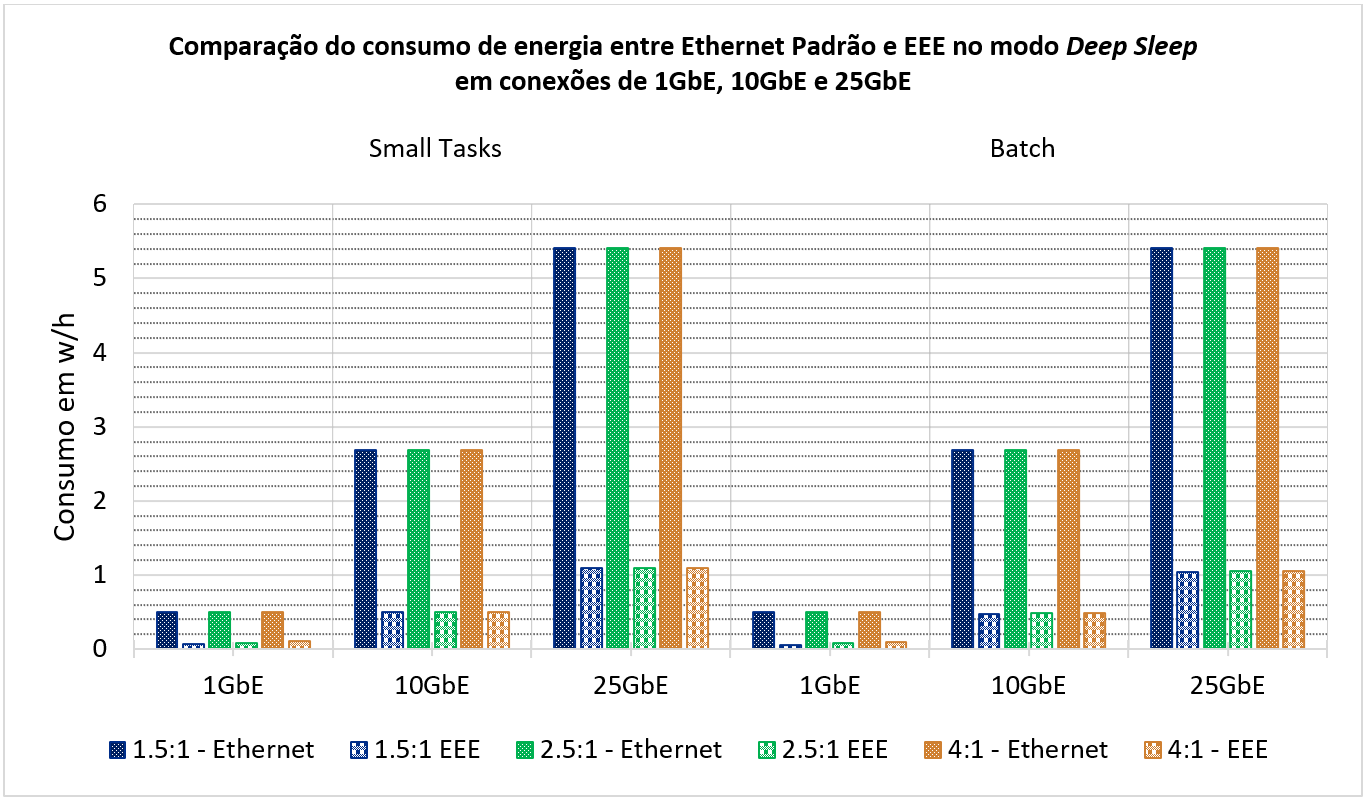
\includegraphics[width=16cm]{4-EEEHadoop/Image1_EEEConsumption1-10-25.PNG}
    \caption{\centering Comparação do consumo de energia entre \emph{Ethernet} Padrão e EEE no modo \emph{Deep Sleep} em conexões de 1GbE, 10GbE e 25GbE}
    \label{fig:EEEConsumption1-10-25}
\end{figure}

\begin{figure}[htp]
    \centering
    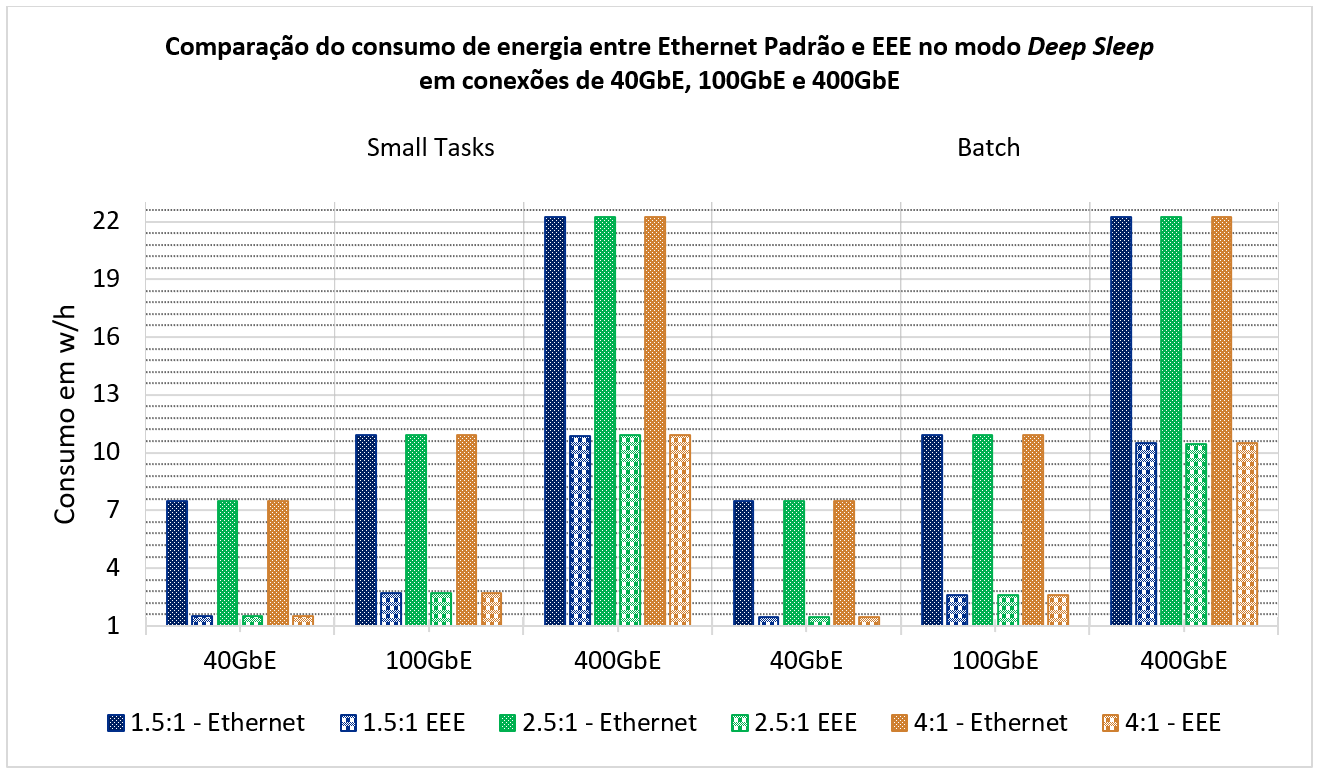
\includegraphics[width=16cm]{4-EEEHadoop/Image2_EEEConsumption40-100-400.PNG}
    \caption{\centering Comparação do consumo de energia entre \emph{Ethernet} Padrão e EEE no modo \emph{Deep Sleep} em conexões de 40GbE, 100GbE e 400GbE}
    \label{fig:EEEConsumption40-100-400}
\end{figure}

\begin{figure}[htp]
    \centering
    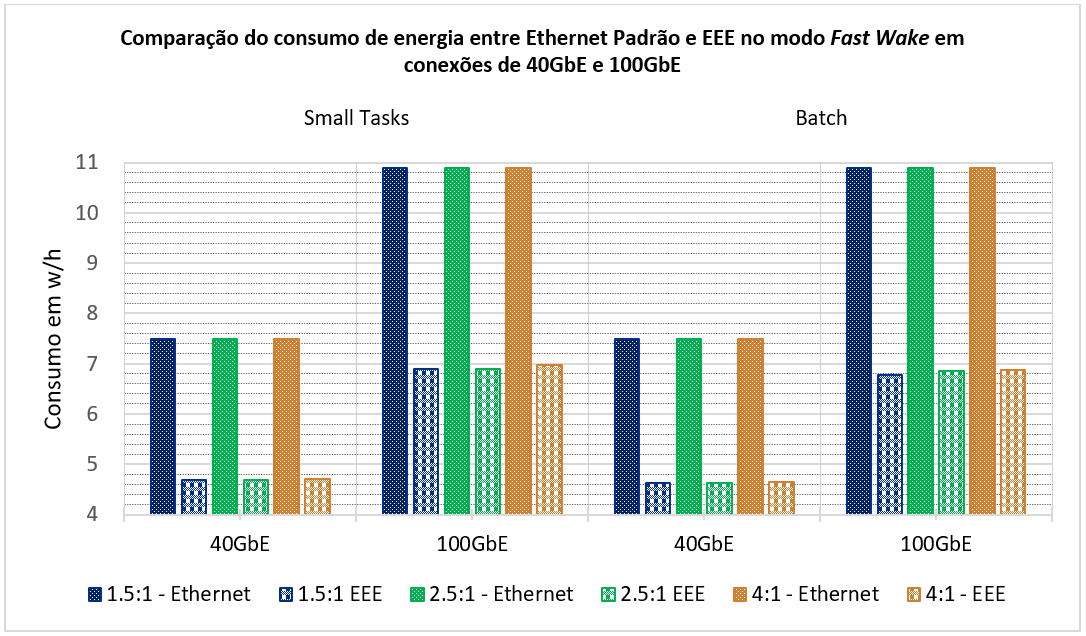
\includegraphics[width=16cm]{4-EEEHadoop/Image5_EEEConsumption40-100-FastWakeMode.PNG}
    \caption{\centering Comparação do consumo de energia entre \emph{Ethernet} Padrão e EEE no modo \emph{Fast Wake} em conexões de 40GbE e 100GbE}
    \label{fig:EEEConsumption100-400FastWakeMode}
\end{figure}

Através das simulações com o modo \textbf{\emph{Deep Sleep}} do EEE encontramos os dados mostrados nas figuras 4.1 e 4.2, que demonstram a economia de energia em \emph{Jobs MapReduce} em \emph{clusters}{} Hadoop 3.x, com reduções médias de 0,5w/h para 0,080w/h em links de 1GbE - redução de 83,89\%; 2,68w/h para 0,490w/h em 10GbE - redução de 81,68\%; de 5,41w/h para 1,072w/h em 25GbE - redução de 80,12\%; 7,49w/h para 1,487w/h em 40GbE - redução de 80,14\%; de 10,89w/h para 2,646w/h em 100GbE - redução de 75,69\%; e de 22,21w/h para 10,685w/h em 400GbE - redução de 51,89.

Usando a configuração de topologia de rede \emph{leaf-spine} recomendada pela Cisco, com uma taxa de assinatura excessiva igual a 4:1, encontramos resultados que, como em \cite{silva2018eon}; \cite{e2015exploring}; \cite{e2017energy}, apontam para economias de energia semelhantes habilitando o EEE no modo \textbf{\emph{Deep Sleep}} ao executar \emph{Small Tasks} e \emph{Batch Jobs}, no entanto, os \emph{Batch Jobs} tiveram um desempenho ligeiramente melhor.

Como pode-se observar na figura 4.3, ao habitarmos o EEE no modo \textbf{\emph{Fast Wake}} para as conexões de 40GbE e 100GbE, percebe-se uma economia de energia relativamente menor do que comparado ao modo \textbf{\emph{Deep Sleep}}, de 7,49w/h para 4,634w/h em conexões de 40GbE - redução de 38,13\%, e de 10,89w/h para 6,916w/h - redução de 36,49\% em conexões de 100GbE respectivamente. Em contrapartida, o desempenho foi melhor como detalhado na próxima seção.

\section{Desempenho}

Esta seção contém os dados de performance obtidos das simulações com topologia \emph{leaf-spine} e conexões de 1GbE e 10GbE; 1GbE e 25GbE; 10GbE e 100GbE; 10GbE e 400GbE; 25GbE e 400GbE; e, finalmente, 40GbE e 400GbE. O restante da metodologia empregada pode ser visualizada no Capítulo 3 de forma detalhada.

Ao contrário do que afirmam os fornecedores de equipamentos, nossos testes demonstram que é possível obter uma boa economia de energia habilitando o \emph{Energy Efficient Ethernet} no modo \textbf{\emph{Deep Sleep}}, com uma perda média de desempenho de praticamente zero para links de 1GbE - 0,21\%; 10GbE - 0,94\%; e 25GbE - 1,52\%; ou razoável no caso de 40GbE - 2,85\% conforme mostrado nas figuras 4.4 e 4.5. Para links de 100GbE e 400GbE há uma boa economia de energia, mas com uma perda de desempenho que não é considerada ideal, em torno de 4,55\% e 8,58\% respectivamente.

Em geral, ao habilitar o EEE em modo \textbf{\emph{Deep Sleep}} no \emph{cluster}, percebe-se que os \emph{Batch Jobs} obtêm melhor economia de energia e desempenho em relação aos \emph{Small Tasks}. Ainda é possível observar um cenário específico, em que ao diminuir a taxa de assinatura excessiva da rede para 1.5:1 em links 1GbE, os \emph{Batch Jobs} obtiveram uma melhora significativamente maior na economia de energia e no desempenho em comparação com outras conexões.

\begin{figure}[htp]
    \centering
    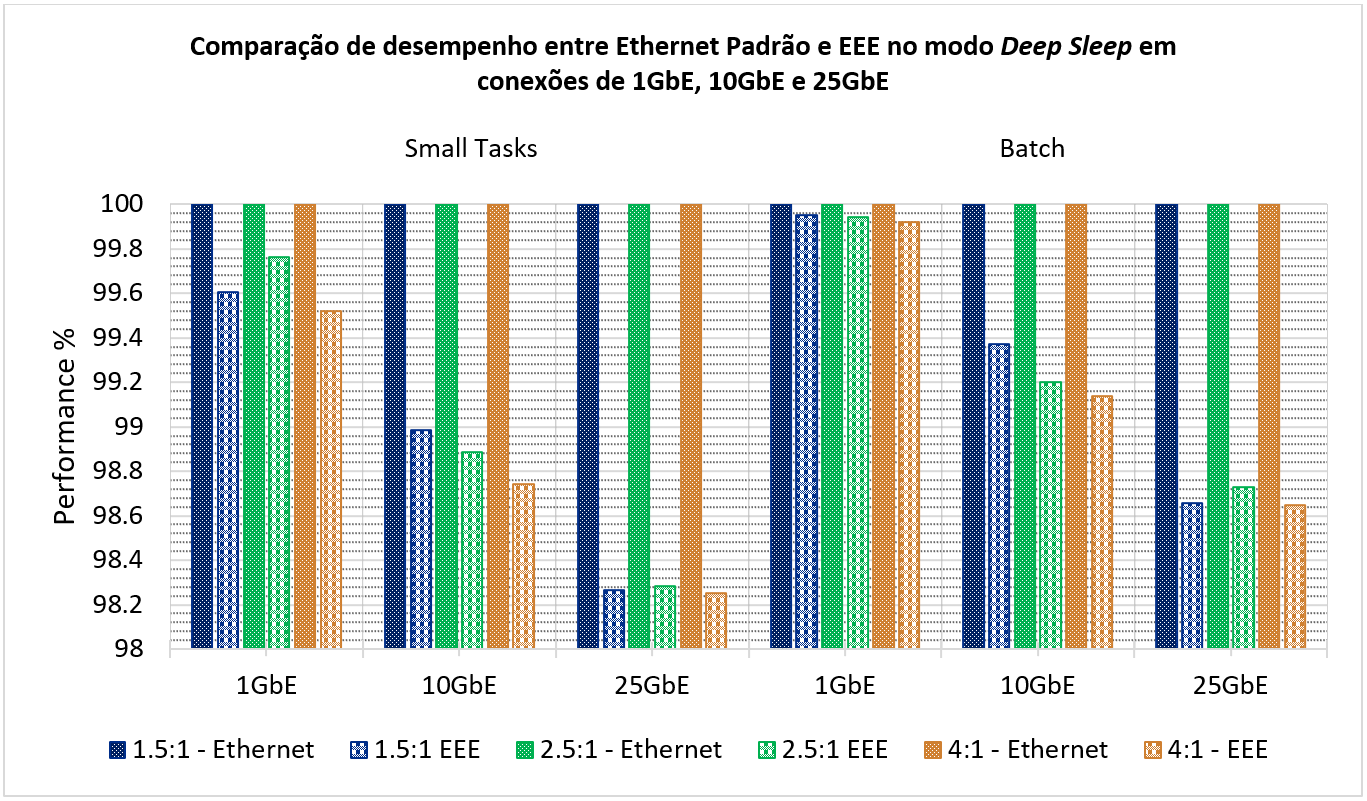
\includegraphics[width=16cm]{4-EEEHadoop/Image3_EEEPerformance1-10-25.PNG}
    \caption{\centering Comparação de desempenho entre \emph{Ethernet} Padrão e EEE no modo \emph{Deep Sleep} em conexões de 1GbE, 10GbE e 25GbE}
    \label{fig:EEEPerformance1-10-25}
\end{figure}

\begin{figure}[htp]
    \centering
    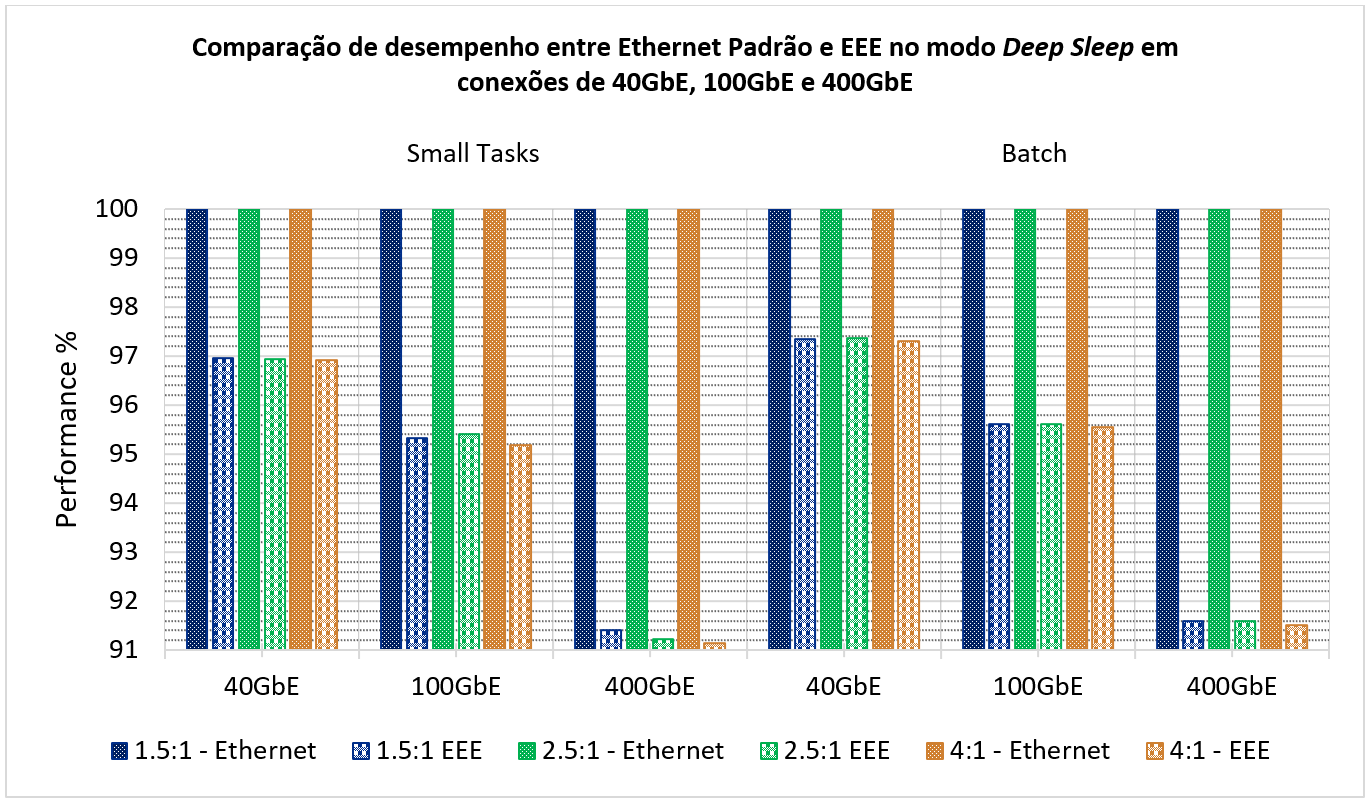
\includegraphics[width=16cm]{4-EEEHadoop/Image4_EEEPerformance40-100-400.PNG}
    \caption{\centering Comparação de desempenho entre \emph{Ethernet} Padrão e EEE no modo \emph{Deep Sleep} em conexões de 40GbE, 100GbE e 400GbE}
    \label{fig:EEEPerformance40-100-400}
\end{figure}

\begin{figure}[htp]
    \centering
    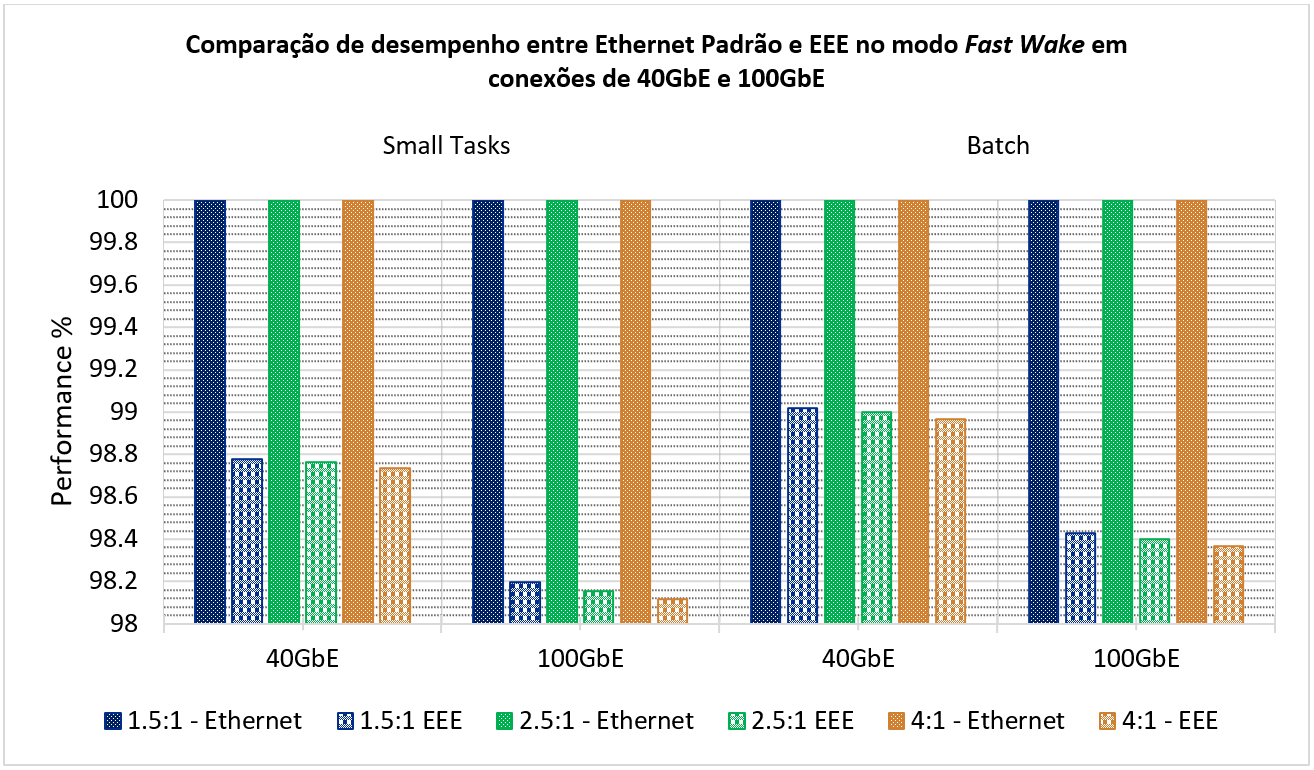
\includegraphics[width=16cm]{4-EEEHadoop/Image6_EEEPerformance40-100-FastWakeMode.PNG}
    \caption{\centering Comparação de desempenho entre \emph{Ethernet} Padrão e EEE no modo \emph{Fast Wake} em conexões de 40GbE e 100GbE}
    \label{fig:EEEPerformance40-100FastWake}
\end{figure}

Ao utilizarmos o modo \textbf{\emph{Fast Wake}} do EEE em nossas simulações, foi possível notar que embora este modo não forneça uma economia de energia como o modo \textbf{\emph{Deep Sleep}}, ele não afeta o desempenho de forma que seja considerável, com uma perda de 1,2\% no caso das conexões de 40GbE e 1,8\% em conexões de 100GbE, tornando-se assim uma opção interessante para as indústrias que buscam um balanceamento entre economia de energia e desempenho.  

As perdas de desempenho mais significativas encontradas para os links de 100GbE e 400GbE com o modo \textbf{\emph{Deep Sleep}} ocorreram porque em determinados momentos é necessário acordar um link para transmitir um único \emph{frame}, o que causa penalidades de latência e consumo de energia em termos relativos que são agravadas de acordo com a largura de banda \cite{jiang2021modeling}; \cite{reviriego2009performance}; \cite{reviriego2010burst}; \cite{e2017energy}. Se os momentos de \emph{wake} do EEE puderem ser controlados para evitar transmissões de um \emph{frame} único, pode ser possível obter economia de energia com perdas de desempenho baixas ou nulas para estas conexões.

\section{Considerações Finais}

Neste capítulo, apresentamos uma análise do impacto ao habilitar ao \emph{Energy Efficient Ethernet} nos modos \textbf{\emph{Deep Sleep}} e \textbf{\emph{Fast Wake}} em \emph{clusters MapReduce} que utilizam o \emph{framework} Apache Hadoop 3.x. Avaliamos execuções de \emph{Small Tasks} e \emph{Batch Jobs} com EEE em diversos \emph{clusters} simulados, e no modo \textbf{\emph{Deep Sleep}} encontramos economia de energia entre 78\% e 82\% para links de até 40GbE sem perda considerável de desempenho, entre 0,21\% e 2,85 \%. Para links de 100GbE e 400GbE houve uma economia de energia significativa de 75,69\% e 51,88\% respectivamente, mas com uma taxa de perda de desempenho considerável de 4,55\% e 8,58\%, o que não é particularmente interessante em \emph{Batch Jobs}. Quando optamos pelo uso do modo \textbf{\emph{Fast Wake}} do EEE, obtivemos uma redução do consumo de 7,49w/h para 4,634w/h em conexões de 40GbE, e de 10,89w/h para 6,916w/h em conexões de 100GbE, com uma perda de performance de 1.2\% e 1.8\%.

Em termos de custo-benefício para \emph{data centers}, o recomendado para conexões de até 40GbE é habilitar o EEE no modo \textbf{\emph{Deep Sleep}}, o que resulta em uma boa redução do consumo de energia e uma taxa de perda de desempenho baixa ou nula. Para conexões de 100GbE o recomendado é habilitar o modo \textbf{\emph{Fast Wake}} do EEE, obtendo assim um balanceamento entre consumo de energia e performance. Para conexões de 400GbE habilitar o EEE não é interessante, pois há uma perda de 8,58\% do desempenho.

O problema de latência e economia de energia encontrado em conexões acima de 100GbE com \textbf{\emph{Deep Sleep}} são causados por ter que acordar o link de tempos em tempos para transmitir um único \emph{frame}. Para resolver este problema, no próximo capítulo combinamos o \emph{Energy Efficient Ethernet} com \emph{Packet Coalescing}, \emph{Random Early Detection}, \emph{Controlled Delay}  e \emph{Explicit Congestion Notification}, podendo assim configurar de forma manual e inteligente quando os links devem ser acordados do modo LPI para transmissões de pacotes.

	% conclusão

%=====================================================

% Estilos de bibliografia recomendados (só descomentar um estilo!)
% Mais infos: https://pt.sharelatex.com/learn/Bibtex_bibliography_styles
%
% ATENÇÃO: evite usar \cite{}; prefira \citep{} e \citet{}
%
\bibliographystyle{apalike-ptbr}	% [Maziero et al., 2006]
%\bibliographystyle{alpha}		% [Maz06]
%\bibliographystyle{plainnat}		% vide Google "LaTeX Natbib"
%\bibliographystyle{plain}		% [1] ordem alfabética
%\bibliographystyle{unsrt}		% [1] ordem de uso no texto

% no estilo "unsrt", evita que citações nos índices sejam consideradas
%\usepackage{notoccite}

% base de bibliografia (BibTeX)
\bibliography{referencias}
%\bibliography{file1,file2,file3} % se tiver mais de um arquivo BibTeX

%=====================================================

% inclusão de apêndices
% \appendix

% inclusão de apêndice
% \chapter{Energy Efficient Ethernet em Clusters Hadoop MapReduce}

Neste capítulo são apresentados os resultados das simulações de \emph{clusters Hadoop 3.x MapReduce} utilizando a ferramenta NetSLS e o \emph{Energy Efficient Ethernet} em modo \emph{Fast Wake} e \emph{Deep Sleep}. Através destes dados mostramos que uma boa economia de energia pode ser obtida em conexões de até 40GbE, enquanto conexões acima de 100GbE possuem problemas de performance quando o EEE está habilitado no modo \emph{Deep Sleep}.

\section{Economia de Energia}

Esta seção contém os dados de economia de energia obtidos das simulações com topologia \emph{leaf-spine} e conexões de 1GbE e 10GbE; 1GbE e 25GbE; 10GbE e 100GbE; 10GbE e 400GbE; 25GbE e 400GbE; e, finalmente, 40GbE e 400GbE. O restante da metodologia empregada pode ser visualizada no Capítulo 3 de forma detalhada.

\begin{figure}[htp]
    \centering
    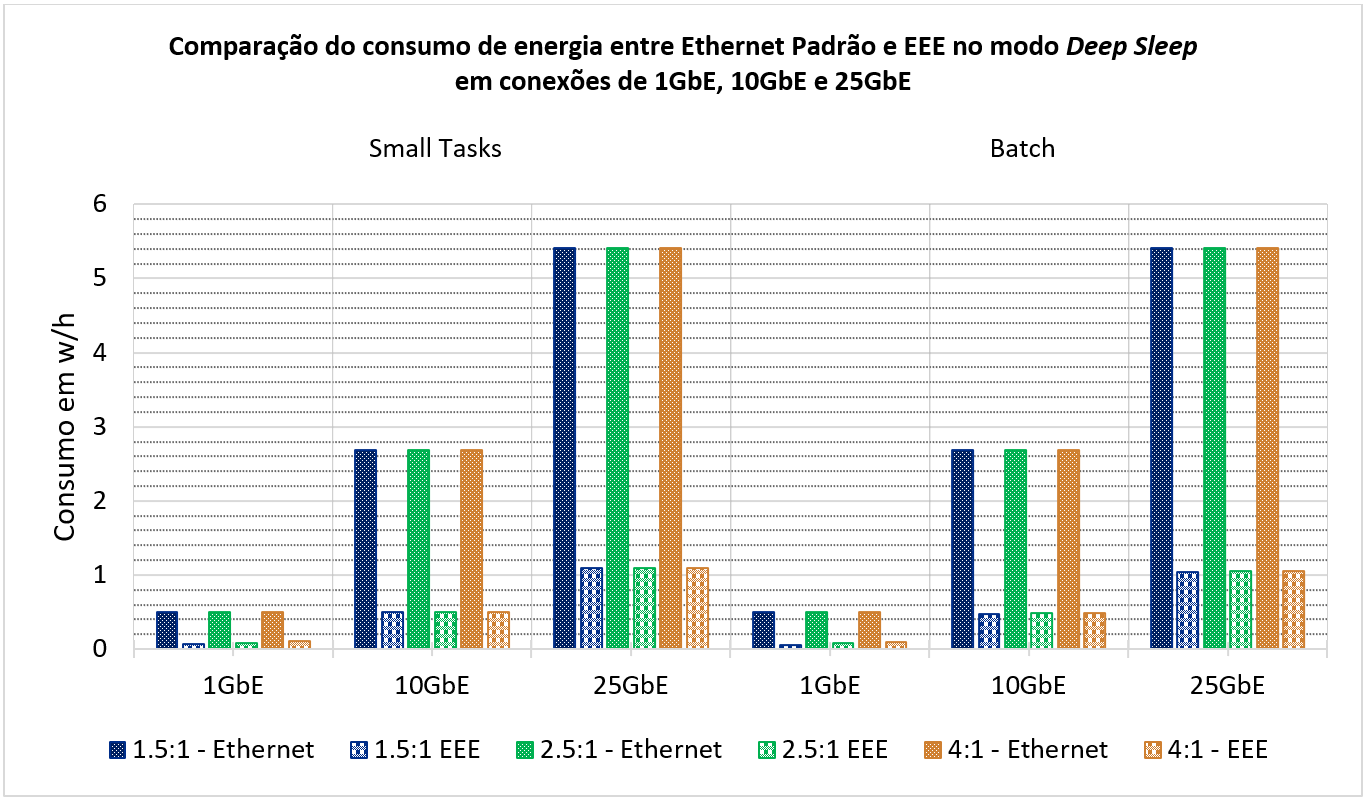
\includegraphics[width=16cm]{4-EEEHadoop/Image1_EEEConsumption1-10-25.PNG}
    \caption{\centering Comparação do consumo de energia entre \emph{Ethernet} Padrão e EEE no modo \emph{Deep Sleep} em conexões de 1GbE, 10GbE e 25GbE}
    \label{fig:EEEConsumption1-10-25}
\end{figure}

\begin{figure}[htp]
    \centering
    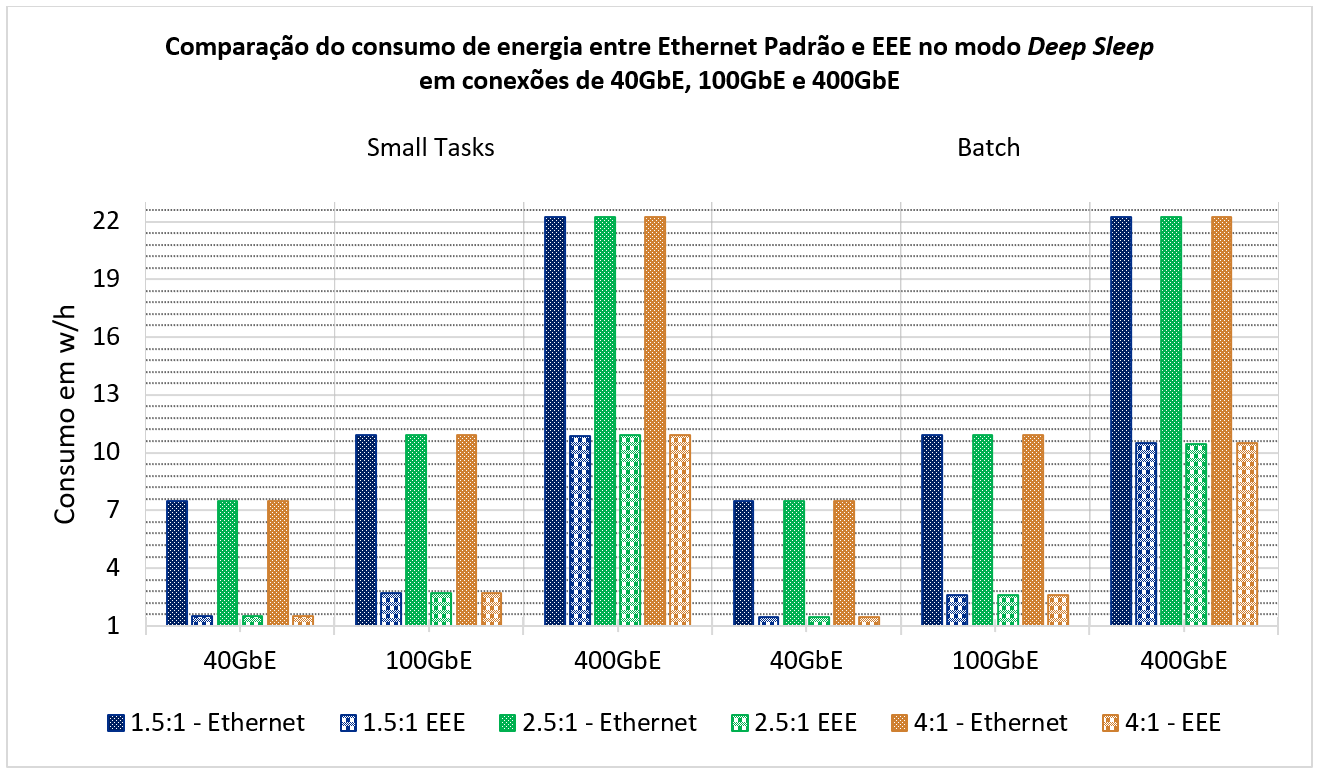
\includegraphics[width=16cm]{4-EEEHadoop/Image2_EEEConsumption40-100-400.PNG}
    \caption{\centering Comparação do consumo de energia entre \emph{Ethernet} Padrão e EEE no modo \emph{Deep Sleep} em conexões de 40GbE, 100GbE e 400GbE}
    \label{fig:EEEConsumption40-100-400}
\end{figure}

\begin{figure}[htp]
    \centering
    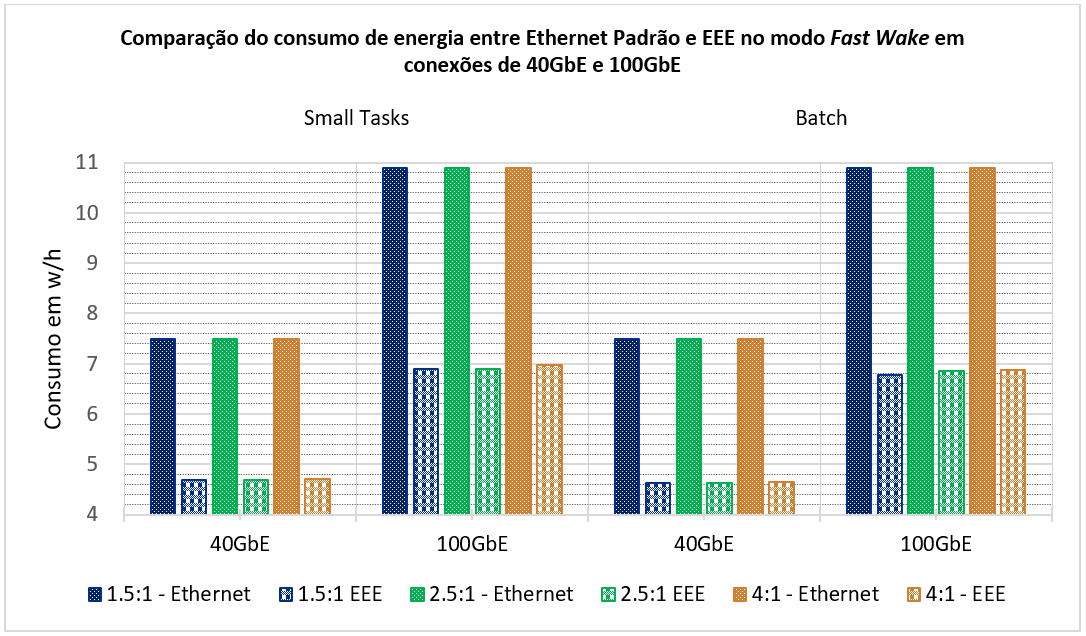
\includegraphics[width=16cm]{4-EEEHadoop/Image5_EEEConsumption40-100-FastWakeMode.PNG}
    \caption{\centering Comparação do consumo de energia entre \emph{Ethernet} Padrão e EEE no modo \emph{Fast Wake} em conexões de 40GbE e 100GbE}
    \label{fig:EEEConsumption100-400FastWakeMode}
\end{figure}

Através das simulações com o modo \textbf{\emph{Deep Sleep}} do EEE encontramos os dados mostrados nas figuras 4.1 e 4.2, que demonstram a economia de energia em \emph{Jobs MapReduce} em \emph{clusters}{} Hadoop 3.x, com reduções médias de 0,5w/h para 0,080w/h em links de 1GbE - redução de 83,89\%; 2,68w/h para 0,490w/h em 10GbE - redução de 81,68\%; de 5,41w/h para 1,072w/h em 25GbE - redução de 80,12\%; 7,49w/h para 1,487w/h em 40GbE - redução de 80,14\%; de 10,89w/h para 2,646w/h em 100GbE - redução de 75,69\%; e de 22,21w/h para 10,685w/h em 400GbE - redução de 51,89.

Usando a configuração de topologia de rede \emph{leaf-spine} recomendada pela Cisco, com uma taxa de assinatura excessiva igual a 4:1, encontramos resultados que, como em \cite{silva2018eon}; \cite{e2015exploring}; \cite{e2017energy}, apontam para economias de energia semelhantes habilitando o EEE no modo \textbf{\emph{Deep Sleep}} ao executar \emph{Small Tasks} e \emph{Batch Jobs}, no entanto, os \emph{Batch Jobs} tiveram um desempenho ligeiramente melhor.

Como pode-se observar na figura 4.3, ao habitarmos o EEE no modo \textbf{\emph{Fast Wake}} para as conexões de 40GbE e 100GbE, percebe-se uma economia de energia relativamente menor do que comparado ao modo \textbf{\emph{Deep Sleep}}, de 7,49w/h para 4,634w/h em conexões de 40GbE - redução de 38,13\%, e de 10,89w/h para 6,916w/h - redução de 36,49\% em conexões de 100GbE respectivamente. Em contrapartida, o desempenho foi melhor como detalhado na próxima seção.

\section{Desempenho}

Esta seção contém os dados de performance obtidos das simulações com topologia \emph{leaf-spine} e conexões de 1GbE e 10GbE; 1GbE e 25GbE; 10GbE e 100GbE; 10GbE e 400GbE; 25GbE e 400GbE; e, finalmente, 40GbE e 400GbE. O restante da metodologia empregada pode ser visualizada no Capítulo 3 de forma detalhada.

Ao contrário do que afirmam os fornecedores de equipamentos, nossos testes demonstram que é possível obter uma boa economia de energia habilitando o \emph{Energy Efficient Ethernet} no modo \textbf{\emph{Deep Sleep}}, com uma perda média de desempenho de praticamente zero para links de 1GbE - 0,21\%; 10GbE - 0,94\%; e 25GbE - 1,52\%; ou razoável no caso de 40GbE - 2,85\% conforme mostrado nas figuras 4.4 e 4.5. Para links de 100GbE e 400GbE há uma boa economia de energia, mas com uma perda de desempenho que não é considerada ideal, em torno de 4,55\% e 8,58\% respectivamente.

Em geral, ao habilitar o EEE em modo \textbf{\emph{Deep Sleep}} no \emph{cluster}, percebe-se que os \emph{Batch Jobs} obtêm melhor economia de energia e desempenho em relação aos \emph{Small Tasks}. Ainda é possível observar um cenário específico, em que ao diminuir a taxa de assinatura excessiva da rede para 1.5:1 em links 1GbE, os \emph{Batch Jobs} obtiveram uma melhora significativamente maior na economia de energia e no desempenho em comparação com outras conexões.

\begin{figure}[htp]
    \centering
    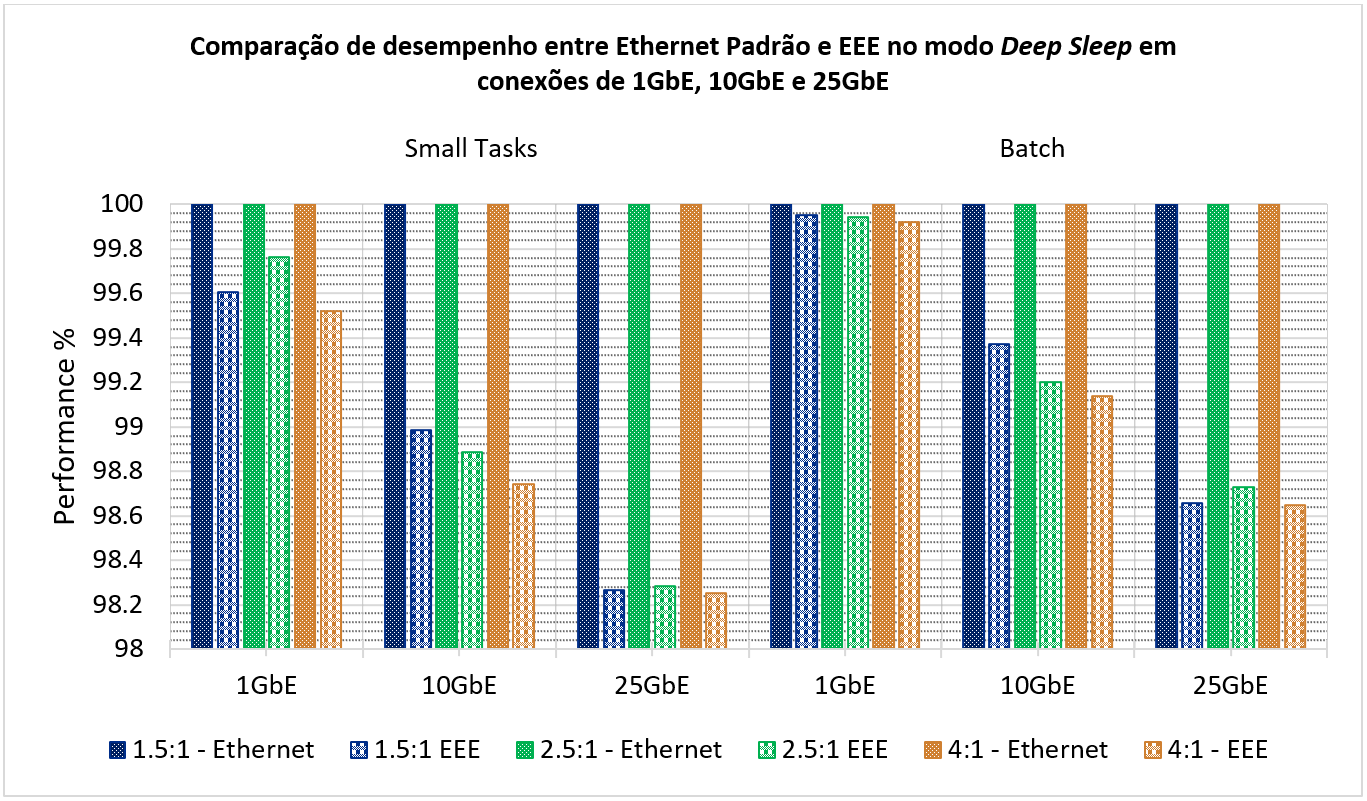
\includegraphics[width=16cm]{4-EEEHadoop/Image3_EEEPerformance1-10-25.PNG}
    \caption{\centering Comparação de desempenho entre \emph{Ethernet} Padrão e EEE no modo \emph{Deep Sleep} em conexões de 1GbE, 10GbE e 25GbE}
    \label{fig:EEEPerformance1-10-25}
\end{figure}

\begin{figure}[htp]
    \centering
    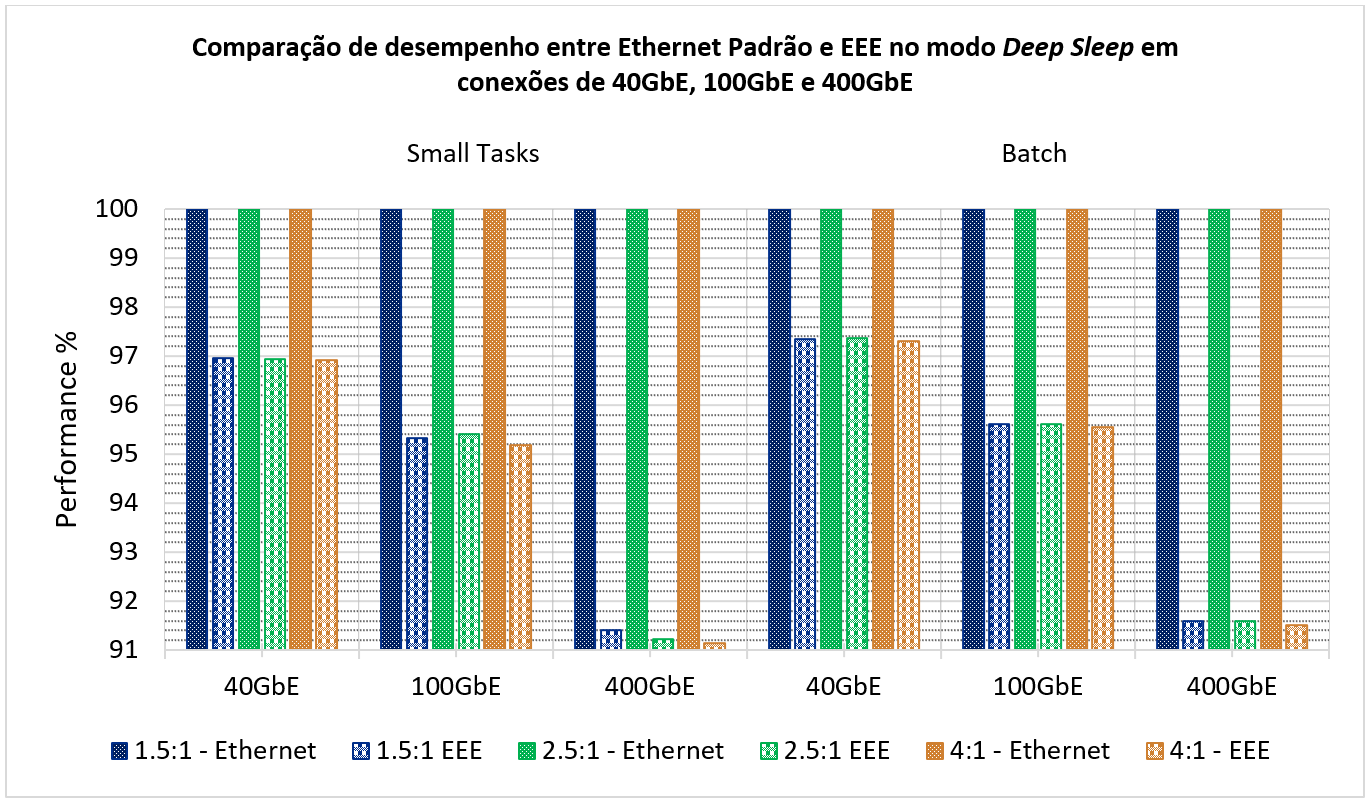
\includegraphics[width=16cm]{4-EEEHadoop/Image4_EEEPerformance40-100-400.PNG}
    \caption{\centering Comparação de desempenho entre \emph{Ethernet} Padrão e EEE no modo \emph{Deep Sleep} em conexões de 40GbE, 100GbE e 400GbE}
    \label{fig:EEEPerformance40-100-400}
\end{figure}

\begin{figure}[htp]
    \centering
    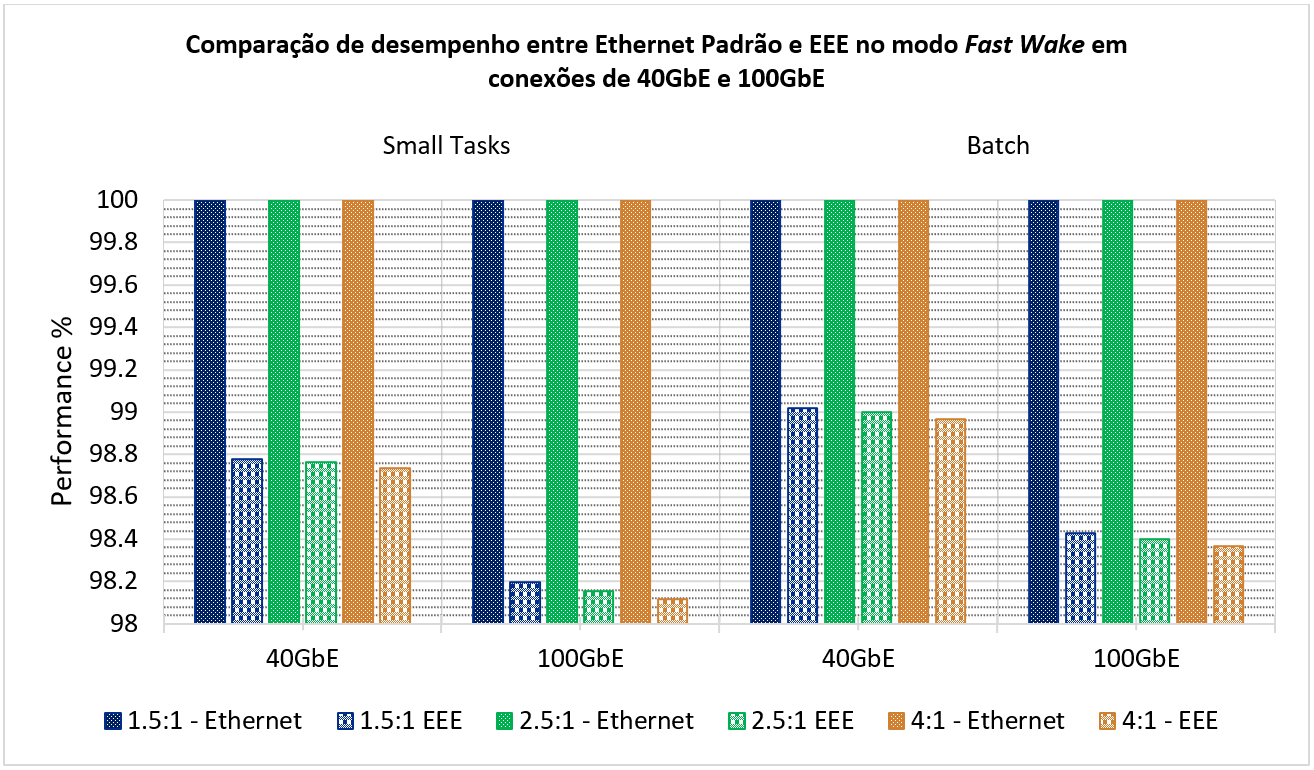
\includegraphics[width=16cm]{4-EEEHadoop/Image6_EEEPerformance40-100-FastWakeMode.PNG}
    \caption{\centering Comparação de desempenho entre \emph{Ethernet} Padrão e EEE no modo \emph{Fast Wake} em conexões de 40GbE e 100GbE}
    \label{fig:EEEPerformance40-100FastWake}
\end{figure}

Ao utilizarmos o modo \textbf{\emph{Fast Wake}} do EEE em nossas simulações, foi possível notar que embora este modo não forneça uma economia de energia como o modo \textbf{\emph{Deep Sleep}}, ele não afeta o desempenho de forma que seja considerável, com uma perda de 1,2\% no caso das conexões de 40GbE e 1,8\% em conexões de 100GbE, tornando-se assim uma opção interessante para as indústrias que buscam um balanceamento entre economia de energia e desempenho.  

As perdas de desempenho mais significativas encontradas para os links de 100GbE e 400GbE com o modo \textbf{\emph{Deep Sleep}} ocorreram porque em determinados momentos é necessário acordar um link para transmitir um único \emph{frame}, o que causa penalidades de latência e consumo de energia em termos relativos que são agravadas de acordo com a largura de banda \cite{jiang2021modeling}; \cite{reviriego2009performance}; \cite{reviriego2010burst}; \cite{e2017energy}. Se os momentos de \emph{wake} do EEE puderem ser controlados para evitar transmissões de um \emph{frame} único, pode ser possível obter economia de energia com perdas de desempenho baixas ou nulas para estas conexões.

\section{Considerações Finais}

Neste capítulo, apresentamos uma análise do impacto ao habilitar ao \emph{Energy Efficient Ethernet} nos modos \textbf{\emph{Deep Sleep}} e \textbf{\emph{Fast Wake}} em \emph{clusters MapReduce} que utilizam o \emph{framework} Apache Hadoop 3.x. Avaliamos execuções de \emph{Small Tasks} e \emph{Batch Jobs} com EEE em diversos \emph{clusters} simulados, e no modo \textbf{\emph{Deep Sleep}} encontramos economia de energia entre 78\% e 82\% para links de até 40GbE sem perda considerável de desempenho, entre 0,21\% e 2,85 \%. Para links de 100GbE e 400GbE houve uma economia de energia significativa de 75,69\% e 51,88\% respectivamente, mas com uma taxa de perda de desempenho considerável de 4,55\% e 8,58\%, o que não é particularmente interessante em \emph{Batch Jobs}. Quando optamos pelo uso do modo \textbf{\emph{Fast Wake}} do EEE, obtivemos uma redução do consumo de 7,49w/h para 4,634w/h em conexões de 40GbE, e de 10,89w/h para 6,916w/h em conexões de 100GbE, com uma perda de performance de 1.2\% e 1.8\%.

Em termos de custo-benefício para \emph{data centers}, o recomendado para conexões de até 40GbE é habilitar o EEE no modo \textbf{\emph{Deep Sleep}}, o que resulta em uma boa redução do consumo de energia e uma taxa de perda de desempenho baixa ou nula. Para conexões de 100GbE o recomendado é habilitar o modo \textbf{\emph{Fast Wake}} do EEE, obtendo assim um balanceamento entre consumo de energia e performance. Para conexões de 400GbE habilitar o EEE não é interessante, pois há uma perda de 8,58\% do desempenho.

O problema de latência e economia de energia encontrado em conexões acima de 100GbE com \textbf{\emph{Deep Sleep}} são causados por ter que acordar o link de tempos em tempos para transmitir um único \emph{frame}. Para resolver este problema, no próximo capítulo combinamos o \emph{Energy Efficient Ethernet} com \emph{Packet Coalescing}, \emph{Random Early Detection}, \emph{Controlled Delay}  e \emph{Explicit Congestion Notification}, podendo assim configurar de forma manual e inteligente quando os links devem ser acordados do modo LPI para transmissões de pacotes.



%=====================================================

\end{document}

%=====================================================
